
% Default to the notebook output style

    


% Inherit from the specified cell style.




    
\documentclass[11pt]{article}

    
    
    \usepackage[T1]{fontenc}
    % Nicer default font (+ math font) than Computer Modern for most use cases
    \usepackage{mathpazo}

    % Basic figure setup, for now with no caption control since it's done
    % automatically by Pandoc (which extracts ![](path) syntax from Markdown).
    \usepackage{graphicx}
    % We will generate all images so they have a width \maxwidth. This means
    % that they will get their normal width if they fit onto the page, but
    % are scaled down if they would overflow the margins.
    \makeatletter
    \def\maxwidth{\ifdim\Gin@nat@width>\linewidth\linewidth
    \else\Gin@nat@width\fi}
    \makeatother
    \let\Oldincludegraphics\includegraphics
    % Set max figure width to be 80% of text width, for now hardcoded.
    \renewcommand{\includegraphics}[1]{\Oldincludegraphics[width=.8\maxwidth]{#1}}
    % Ensure that by default, figures have no caption (until we provide a
    % proper Figure object with a Caption API and a way to capture that
    % in the conversion process - todo).
    \usepackage{caption}
    \DeclareCaptionLabelFormat{nolabel}{}
    \captionsetup{labelformat=nolabel}

    \usepackage{adjustbox} % Used to constrain images to a maximum size 
    \usepackage{xcolor} % Allow colors to be defined
    \usepackage{enumerate} % Needed for markdown enumerations to work
    \usepackage{geometry} % Used to adjust the document margins
    \usepackage{amsmath} % Equations
    \usepackage{amssymb} % Equations
    \usepackage{textcomp} % defines textquotesingle
    % Hack from http://tex.stackexchange.com/a/47451/13684:
    \AtBeginDocument{%
        \def\PYZsq{\textquotesingle}% Upright quotes in Pygmentized code
    }
    \usepackage{upquote} % Upright quotes for verbatim code
    \usepackage{eurosym} % defines \euro
    \usepackage[mathletters]{ucs} % Extended unicode (utf-8) support
    \usepackage[utf8x]{inputenc} % Allow utf-8 characters in the tex document
    \usepackage{fancyvrb} % verbatim replacement that allows latex
    \usepackage{grffile} % extends the file name processing of package graphics 
                         % to support a larger range 
    % The hyperref package gives us a pdf with properly built
    % internal navigation ('pdf bookmarks' for the table of contents,
    % internal cross-reference links, web links for URLs, etc.)
    \usepackage{hyperref}
    \usepackage{longtable} % longtable support required by pandoc >1.10
    \usepackage{booktabs}  % table support for pandoc > 1.12.2
    \usepackage[inline]{enumitem} % IRkernel/repr support (it uses the enumerate* environment)
    \usepackage[normalem]{ulem} % ulem is needed to support strikethroughs (\sout)
                                % normalem makes italics be italics, not underlines
    

    
    
    % Colors for the hyperref package
    \definecolor{urlcolor}{rgb}{0,.145,.698}
    \definecolor{linkcolor}{rgb}{.71,0.21,0.01}
    \definecolor{citecolor}{rgb}{.12,.54,.11}

    % ANSI colors
    \definecolor{ansi-black}{HTML}{3E424D}
    \definecolor{ansi-black-intense}{HTML}{282C36}
    \definecolor{ansi-red}{HTML}{E75C58}
    \definecolor{ansi-red-intense}{HTML}{B22B31}
    \definecolor{ansi-green}{HTML}{00A250}
    \definecolor{ansi-green-intense}{HTML}{007427}
    \definecolor{ansi-yellow}{HTML}{DDB62B}
    \definecolor{ansi-yellow-intense}{HTML}{B27D12}
    \definecolor{ansi-blue}{HTML}{208FFB}
    \definecolor{ansi-blue-intense}{HTML}{0065CA}
    \definecolor{ansi-magenta}{HTML}{D160C4}
    \definecolor{ansi-magenta-intense}{HTML}{A03196}
    \definecolor{ansi-cyan}{HTML}{60C6C8}
    \definecolor{ansi-cyan-intense}{HTML}{258F8F}
    \definecolor{ansi-white}{HTML}{C5C1B4}
    \definecolor{ansi-white-intense}{HTML}{A1A6B2}

    % commands and environments needed by pandoc snippets
    % extracted from the output of `pandoc -s`
    \providecommand{\tightlist}{%
      \setlength{\itemsep}{0pt}\setlength{\parskip}{0pt}}
    \DefineVerbatimEnvironment{Highlighting}{Verbatim}{commandchars=\\\{\}}
    % Add ',fontsize=\small' for more characters per line
    \newenvironment{Shaded}{}{}
    \newcommand{\KeywordTok}[1]{\textcolor[rgb]{0.00,0.44,0.13}{\textbf{{#1}}}}
    \newcommand{\DataTypeTok}[1]{\textcolor[rgb]{0.56,0.13,0.00}{{#1}}}
    \newcommand{\DecValTok}[1]{\textcolor[rgb]{0.25,0.63,0.44}{{#1}}}
    \newcommand{\BaseNTok}[1]{\textcolor[rgb]{0.25,0.63,0.44}{{#1}}}
    \newcommand{\FloatTok}[1]{\textcolor[rgb]{0.25,0.63,0.44}{{#1}}}
    \newcommand{\CharTok}[1]{\textcolor[rgb]{0.25,0.44,0.63}{{#1}}}
    \newcommand{\StringTok}[1]{\textcolor[rgb]{0.25,0.44,0.63}{{#1}}}
    \newcommand{\CommentTok}[1]{\textcolor[rgb]{0.38,0.63,0.69}{\textit{{#1}}}}
    \newcommand{\OtherTok}[1]{\textcolor[rgb]{0.00,0.44,0.13}{{#1}}}
    \newcommand{\AlertTok}[1]{\textcolor[rgb]{1.00,0.00,0.00}{\textbf{{#1}}}}
    \newcommand{\FunctionTok}[1]{\textcolor[rgb]{0.02,0.16,0.49}{{#1}}}
    \newcommand{\RegionMarkerTok}[1]{{#1}}
    \newcommand{\ErrorTok}[1]{\textcolor[rgb]{1.00,0.00,0.00}{\textbf{{#1}}}}
    \newcommand{\NormalTok}[1]{{#1}}
    
    % Additional commands for more recent versions of Pandoc
    \newcommand{\ConstantTok}[1]{\textcolor[rgb]{0.53,0.00,0.00}{{#1}}}
    \newcommand{\SpecialCharTok}[1]{\textcolor[rgb]{0.25,0.44,0.63}{{#1}}}
    \newcommand{\VerbatimStringTok}[1]{\textcolor[rgb]{0.25,0.44,0.63}{{#1}}}
    \newcommand{\SpecialStringTok}[1]{\textcolor[rgb]{0.73,0.40,0.53}{{#1}}}
    \newcommand{\ImportTok}[1]{{#1}}
    \newcommand{\DocumentationTok}[1]{\textcolor[rgb]{0.73,0.13,0.13}{\textit{{#1}}}}
    \newcommand{\AnnotationTok}[1]{\textcolor[rgb]{0.38,0.63,0.69}{\textbf{\textit{{#1}}}}}
    \newcommand{\CommentVarTok}[1]{\textcolor[rgb]{0.38,0.63,0.69}{\textbf{\textit{{#1}}}}}
    \newcommand{\VariableTok}[1]{\textcolor[rgb]{0.10,0.09,0.49}{{#1}}}
    \newcommand{\ControlFlowTok}[1]{\textcolor[rgb]{0.00,0.44,0.13}{\textbf{{#1}}}}
    \newcommand{\OperatorTok}[1]{\textcolor[rgb]{0.40,0.40,0.40}{{#1}}}
    \newcommand{\BuiltInTok}[1]{{#1}}
    \newcommand{\ExtensionTok}[1]{{#1}}
    \newcommand{\PreprocessorTok}[1]{\textcolor[rgb]{0.74,0.48,0.00}{{#1}}}
    \newcommand{\AttributeTok}[1]{\textcolor[rgb]{0.49,0.56,0.16}{{#1}}}
    \newcommand{\InformationTok}[1]{\textcolor[rgb]{0.38,0.63,0.69}{\textbf{\textit{{#1}}}}}
    \newcommand{\WarningTok}[1]{\textcolor[rgb]{0.38,0.63,0.69}{\textbf{\textit{{#1}}}}}
    
    
    % Define a nice break command that doesn't care if a line doesn't already
    % exist.
    \def\br{\hspace*{\fill} \\* }
    % Math Jax compatability definitions
    \def\gt{>}
    \def\lt{<}
    % Document parameters
    \title{Full Report}
    
    
    

    % Pygments definitions
    
\makeatletter
\def\PY@reset{\let\PY@it=\relax \let\PY@bf=\relax%
    \let\PY@ul=\relax \let\PY@tc=\relax%
    \let\PY@bc=\relax \let\PY@ff=\relax}
\def\PY@tok#1{\csname PY@tok@#1\endcsname}
\def\PY@toks#1+{\ifx\relax#1\empty\else%
    \PY@tok{#1}\expandafter\PY@toks\fi}
\def\PY@do#1{\PY@bc{\PY@tc{\PY@ul{%
    \PY@it{\PY@bf{\PY@ff{#1}}}}}}}
\def\PY#1#2{\PY@reset\PY@toks#1+\relax+\PY@do{#2}}

\expandafter\def\csname PY@tok@s2\endcsname{\def\PY@tc##1{\textcolor[rgb]{0.73,0.13,0.13}{##1}}}
\expandafter\def\csname PY@tok@k\endcsname{\let\PY@bf=\textbf\def\PY@tc##1{\textcolor[rgb]{0.00,0.50,0.00}{##1}}}
\expandafter\def\csname PY@tok@kc\endcsname{\let\PY@bf=\textbf\def\PY@tc##1{\textcolor[rgb]{0.00,0.50,0.00}{##1}}}
\expandafter\def\csname PY@tok@sd\endcsname{\let\PY@it=\textit\def\PY@tc##1{\textcolor[rgb]{0.73,0.13,0.13}{##1}}}
\expandafter\def\csname PY@tok@s1\endcsname{\def\PY@tc##1{\textcolor[rgb]{0.73,0.13,0.13}{##1}}}
\expandafter\def\csname PY@tok@sr\endcsname{\def\PY@tc##1{\textcolor[rgb]{0.73,0.40,0.53}{##1}}}
\expandafter\def\csname PY@tok@si\endcsname{\let\PY@bf=\textbf\def\PY@tc##1{\textcolor[rgb]{0.73,0.40,0.53}{##1}}}
\expandafter\def\csname PY@tok@nd\endcsname{\def\PY@tc##1{\textcolor[rgb]{0.67,0.13,1.00}{##1}}}
\expandafter\def\csname PY@tok@ss\endcsname{\def\PY@tc##1{\textcolor[rgb]{0.10,0.09,0.49}{##1}}}
\expandafter\def\csname PY@tok@mf\endcsname{\def\PY@tc##1{\textcolor[rgb]{0.40,0.40,0.40}{##1}}}
\expandafter\def\csname PY@tok@c\endcsname{\let\PY@it=\textit\def\PY@tc##1{\textcolor[rgb]{0.25,0.50,0.50}{##1}}}
\expandafter\def\csname PY@tok@na\endcsname{\def\PY@tc##1{\textcolor[rgb]{0.49,0.56,0.16}{##1}}}
\expandafter\def\csname PY@tok@gr\endcsname{\def\PY@tc##1{\textcolor[rgb]{1.00,0.00,0.00}{##1}}}
\expandafter\def\csname PY@tok@nt\endcsname{\let\PY@bf=\textbf\def\PY@tc##1{\textcolor[rgb]{0.00,0.50,0.00}{##1}}}
\expandafter\def\csname PY@tok@sc\endcsname{\def\PY@tc##1{\textcolor[rgb]{0.73,0.13,0.13}{##1}}}
\expandafter\def\csname PY@tok@sx\endcsname{\def\PY@tc##1{\textcolor[rgb]{0.00,0.50,0.00}{##1}}}
\expandafter\def\csname PY@tok@gp\endcsname{\let\PY@bf=\textbf\def\PY@tc##1{\textcolor[rgb]{0.00,0.00,0.50}{##1}}}
\expandafter\def\csname PY@tok@vm\endcsname{\def\PY@tc##1{\textcolor[rgb]{0.10,0.09,0.49}{##1}}}
\expandafter\def\csname PY@tok@c1\endcsname{\let\PY@it=\textit\def\PY@tc##1{\textcolor[rgb]{0.25,0.50,0.50}{##1}}}
\expandafter\def\csname PY@tok@gh\endcsname{\let\PY@bf=\textbf\def\PY@tc##1{\textcolor[rgb]{0.00,0.00,0.50}{##1}}}
\expandafter\def\csname PY@tok@nl\endcsname{\def\PY@tc##1{\textcolor[rgb]{0.63,0.63,0.00}{##1}}}
\expandafter\def\csname PY@tok@gt\endcsname{\def\PY@tc##1{\textcolor[rgb]{0.00,0.27,0.87}{##1}}}
\expandafter\def\csname PY@tok@go\endcsname{\def\PY@tc##1{\textcolor[rgb]{0.53,0.53,0.53}{##1}}}
\expandafter\def\csname PY@tok@kt\endcsname{\def\PY@tc##1{\textcolor[rgb]{0.69,0.00,0.25}{##1}}}
\expandafter\def\csname PY@tok@dl\endcsname{\def\PY@tc##1{\textcolor[rgb]{0.73,0.13,0.13}{##1}}}
\expandafter\def\csname PY@tok@kr\endcsname{\let\PY@bf=\textbf\def\PY@tc##1{\textcolor[rgb]{0.00,0.50,0.00}{##1}}}
\expandafter\def\csname PY@tok@s\endcsname{\def\PY@tc##1{\textcolor[rgb]{0.73,0.13,0.13}{##1}}}
\expandafter\def\csname PY@tok@gi\endcsname{\def\PY@tc##1{\textcolor[rgb]{0.00,0.63,0.00}{##1}}}
\expandafter\def\csname PY@tok@il\endcsname{\def\PY@tc##1{\textcolor[rgb]{0.40,0.40,0.40}{##1}}}
\expandafter\def\csname PY@tok@nf\endcsname{\def\PY@tc##1{\textcolor[rgb]{0.00,0.00,1.00}{##1}}}
\expandafter\def\csname PY@tok@mo\endcsname{\def\PY@tc##1{\textcolor[rgb]{0.40,0.40,0.40}{##1}}}
\expandafter\def\csname PY@tok@m\endcsname{\def\PY@tc##1{\textcolor[rgb]{0.40,0.40,0.40}{##1}}}
\expandafter\def\csname PY@tok@w\endcsname{\def\PY@tc##1{\textcolor[rgb]{0.73,0.73,0.73}{##1}}}
\expandafter\def\csname PY@tok@gs\endcsname{\let\PY@bf=\textbf}
\expandafter\def\csname PY@tok@mi\endcsname{\def\PY@tc##1{\textcolor[rgb]{0.40,0.40,0.40}{##1}}}
\expandafter\def\csname PY@tok@kp\endcsname{\def\PY@tc##1{\textcolor[rgb]{0.00,0.50,0.00}{##1}}}
\expandafter\def\csname PY@tok@gu\endcsname{\let\PY@bf=\textbf\def\PY@tc##1{\textcolor[rgb]{0.50,0.00,0.50}{##1}}}
\expandafter\def\csname PY@tok@bp\endcsname{\def\PY@tc##1{\textcolor[rgb]{0.00,0.50,0.00}{##1}}}
\expandafter\def\csname PY@tok@cp\endcsname{\def\PY@tc##1{\textcolor[rgb]{0.74,0.48,0.00}{##1}}}
\expandafter\def\csname PY@tok@cm\endcsname{\let\PY@it=\textit\def\PY@tc##1{\textcolor[rgb]{0.25,0.50,0.50}{##1}}}
\expandafter\def\csname PY@tok@ow\endcsname{\let\PY@bf=\textbf\def\PY@tc##1{\textcolor[rgb]{0.67,0.13,1.00}{##1}}}
\expandafter\def\csname PY@tok@vi\endcsname{\def\PY@tc##1{\textcolor[rgb]{0.10,0.09,0.49}{##1}}}
\expandafter\def\csname PY@tok@ch\endcsname{\let\PY@it=\textit\def\PY@tc##1{\textcolor[rgb]{0.25,0.50,0.50}{##1}}}
\expandafter\def\csname PY@tok@nb\endcsname{\def\PY@tc##1{\textcolor[rgb]{0.00,0.50,0.00}{##1}}}
\expandafter\def\csname PY@tok@sb\endcsname{\def\PY@tc##1{\textcolor[rgb]{0.73,0.13,0.13}{##1}}}
\expandafter\def\csname PY@tok@se\endcsname{\let\PY@bf=\textbf\def\PY@tc##1{\textcolor[rgb]{0.73,0.40,0.13}{##1}}}
\expandafter\def\csname PY@tok@sh\endcsname{\def\PY@tc##1{\textcolor[rgb]{0.73,0.13,0.13}{##1}}}
\expandafter\def\csname PY@tok@ne\endcsname{\let\PY@bf=\textbf\def\PY@tc##1{\textcolor[rgb]{0.82,0.25,0.23}{##1}}}
\expandafter\def\csname PY@tok@vc\endcsname{\def\PY@tc##1{\textcolor[rgb]{0.10,0.09,0.49}{##1}}}
\expandafter\def\csname PY@tok@kd\endcsname{\let\PY@bf=\textbf\def\PY@tc##1{\textcolor[rgb]{0.00,0.50,0.00}{##1}}}
\expandafter\def\csname PY@tok@mh\endcsname{\def\PY@tc##1{\textcolor[rgb]{0.40,0.40,0.40}{##1}}}
\expandafter\def\csname PY@tok@o\endcsname{\def\PY@tc##1{\textcolor[rgb]{0.40,0.40,0.40}{##1}}}
\expandafter\def\csname PY@tok@no\endcsname{\def\PY@tc##1{\textcolor[rgb]{0.53,0.00,0.00}{##1}}}
\expandafter\def\csname PY@tok@kn\endcsname{\let\PY@bf=\textbf\def\PY@tc##1{\textcolor[rgb]{0.00,0.50,0.00}{##1}}}
\expandafter\def\csname PY@tok@nc\endcsname{\let\PY@bf=\textbf\def\PY@tc##1{\textcolor[rgb]{0.00,0.00,1.00}{##1}}}
\expandafter\def\csname PY@tok@ni\endcsname{\let\PY@bf=\textbf\def\PY@tc##1{\textcolor[rgb]{0.60,0.60,0.60}{##1}}}
\expandafter\def\csname PY@tok@mb\endcsname{\def\PY@tc##1{\textcolor[rgb]{0.40,0.40,0.40}{##1}}}
\expandafter\def\csname PY@tok@nv\endcsname{\def\PY@tc##1{\textcolor[rgb]{0.10,0.09,0.49}{##1}}}
\expandafter\def\csname PY@tok@vg\endcsname{\def\PY@tc##1{\textcolor[rgb]{0.10,0.09,0.49}{##1}}}
\expandafter\def\csname PY@tok@ge\endcsname{\let\PY@it=\textit}
\expandafter\def\csname PY@tok@cpf\endcsname{\let\PY@it=\textit\def\PY@tc##1{\textcolor[rgb]{0.25,0.50,0.50}{##1}}}
\expandafter\def\csname PY@tok@gd\endcsname{\def\PY@tc##1{\textcolor[rgb]{0.63,0.00,0.00}{##1}}}
\expandafter\def\csname PY@tok@nn\endcsname{\let\PY@bf=\textbf\def\PY@tc##1{\textcolor[rgb]{0.00,0.00,1.00}{##1}}}
\expandafter\def\csname PY@tok@sa\endcsname{\def\PY@tc##1{\textcolor[rgb]{0.73,0.13,0.13}{##1}}}
\expandafter\def\csname PY@tok@fm\endcsname{\def\PY@tc##1{\textcolor[rgb]{0.00,0.00,1.00}{##1}}}
\expandafter\def\csname PY@tok@cs\endcsname{\let\PY@it=\textit\def\PY@tc##1{\textcolor[rgb]{0.25,0.50,0.50}{##1}}}
\expandafter\def\csname PY@tok@err\endcsname{\def\PY@bc##1{\setlength{\fboxsep}{0pt}\fcolorbox[rgb]{1.00,0.00,0.00}{1,1,1}{\strut ##1}}}

\def\PYZbs{\char`\\}
\def\PYZus{\char`\_}
\def\PYZob{\char`\{}
\def\PYZcb{\char`\}}
\def\PYZca{\char`\^}
\def\PYZam{\char`\&}
\def\PYZlt{\char`\<}
\def\PYZgt{\char`\>}
\def\PYZsh{\char`\#}
\def\PYZpc{\char`\%}
\def\PYZdl{\char`\$}
\def\PYZhy{\char`\-}
\def\PYZsq{\char`\'}
\def\PYZdq{\char`\"}
\def\PYZti{\char`\~}
% for compatibility with earlier versions
\def\PYZat{@}
\def\PYZlb{[}
\def\PYZrb{]}
\makeatother


    % Exact colors from NB
    \definecolor{incolor}{rgb}{0.0, 0.0, 0.5}
    \definecolor{outcolor}{rgb}{0.545, 0.0, 0.0}



    
    % Prevent overflowing lines due to hard-to-break entities
    \sloppy 
    % Setup hyperref package
    \hypersetup{
      breaklinks=true,  % so long urls are correctly broken across lines
      colorlinks=true,
      urlcolor=urlcolor,
      linkcolor=linkcolor,
      citecolor=citecolor,
      }
    % Slightly bigger margins than the latex defaults
    
    \geometry{verbose,tmargin=1in,bmargin=1in,lmargin=1in,rmargin=1in}
    
    

    \begin{document}
    
    
    \maketitle
    
    

    
    \begin{Verbatim}[commandchars=\\\{\}]
{\color{incolor}In [{\color{incolor}1}]:} \PY{k+kn}{import} \PY{n+nn}{pickle}
        \PY{k+kn}{import} \PY{n+nn}{os}
        \PY{k+kn}{from} \PY{n+nn}{os} \PY{k}{import} \PY{n}{listdir}
        \PY{k+kn}{from} \PY{n+nn}{os}\PY{n+nn}{.}\PY{n+nn}{path} \PY{k}{import} \PY{n}{isfile}\PY{p}{,} \PY{n}{join}
        \PY{k+kn}{import} \PY{n+nn}{numpy} \PY{k}{as} \PY{n+nn}{np}
        \PY{k+kn}{from} \PY{n+nn}{sklearn}\PY{n+nn}{.}\PY{n+nn}{cluster} \PY{k}{import} \PY{n}{KMeans}
        \PY{k+kn}{from} \PY{n+nn}{sklearn}\PY{n+nn}{.}\PY{n+nn}{cluster} \PY{k}{import} \PY{n}{MiniBatchKMeans}
        \PY{k+kn}{import} \PY{n+nn}{time}
        \PY{k+kn}{import} \PY{n+nn}{pandas} \PY{k}{as} \PY{n+nn}{pd}
        \PY{k+kn}{from} \PY{n+nn}{sklearn} \PY{k}{import} \PY{n}{preprocessing}
        \PY{k+kn}{from} \PY{n+nn}{IPython}\PY{n+nn}{.}\PY{n+nn}{display} \PY{k}{import} \PY{n}{Image}
        \PY{k+kn}{from} \PY{n+nn}{IPython}\PY{n+nn}{.}\PY{n+nn}{core}\PY{n+nn}{.}\PY{n+nn}{display} \PY{k}{import} \PY{n}{HTML} 
        
        \PY{c+c1}{\PYZsh{}!pip install memory\PYZus{}profiler}
        \PY{c+c1}{\PYZsh{}\PYZpc{}load\PYZus{}ext memory\PYZus{}profiler}
\end{Verbatim}


    No início do projecto contava com um dataset com 1099 ficheiros audio de
fado extraídos do youtube em formato .wav bem como um conjunto de 3
tipos de features já produzidas pelo Dorin para cada uma das músicas.
Para explorar, visualizei os dados com tsne 2D e 3D. Também limpei o
ficheiro das labels para incluir apenas ID - Nome de Artista - Nome de
canção. Havia também ficheiros muito grandes (álbuns inteiros) que
removi do dataset.

    \begin{figure}
\centering
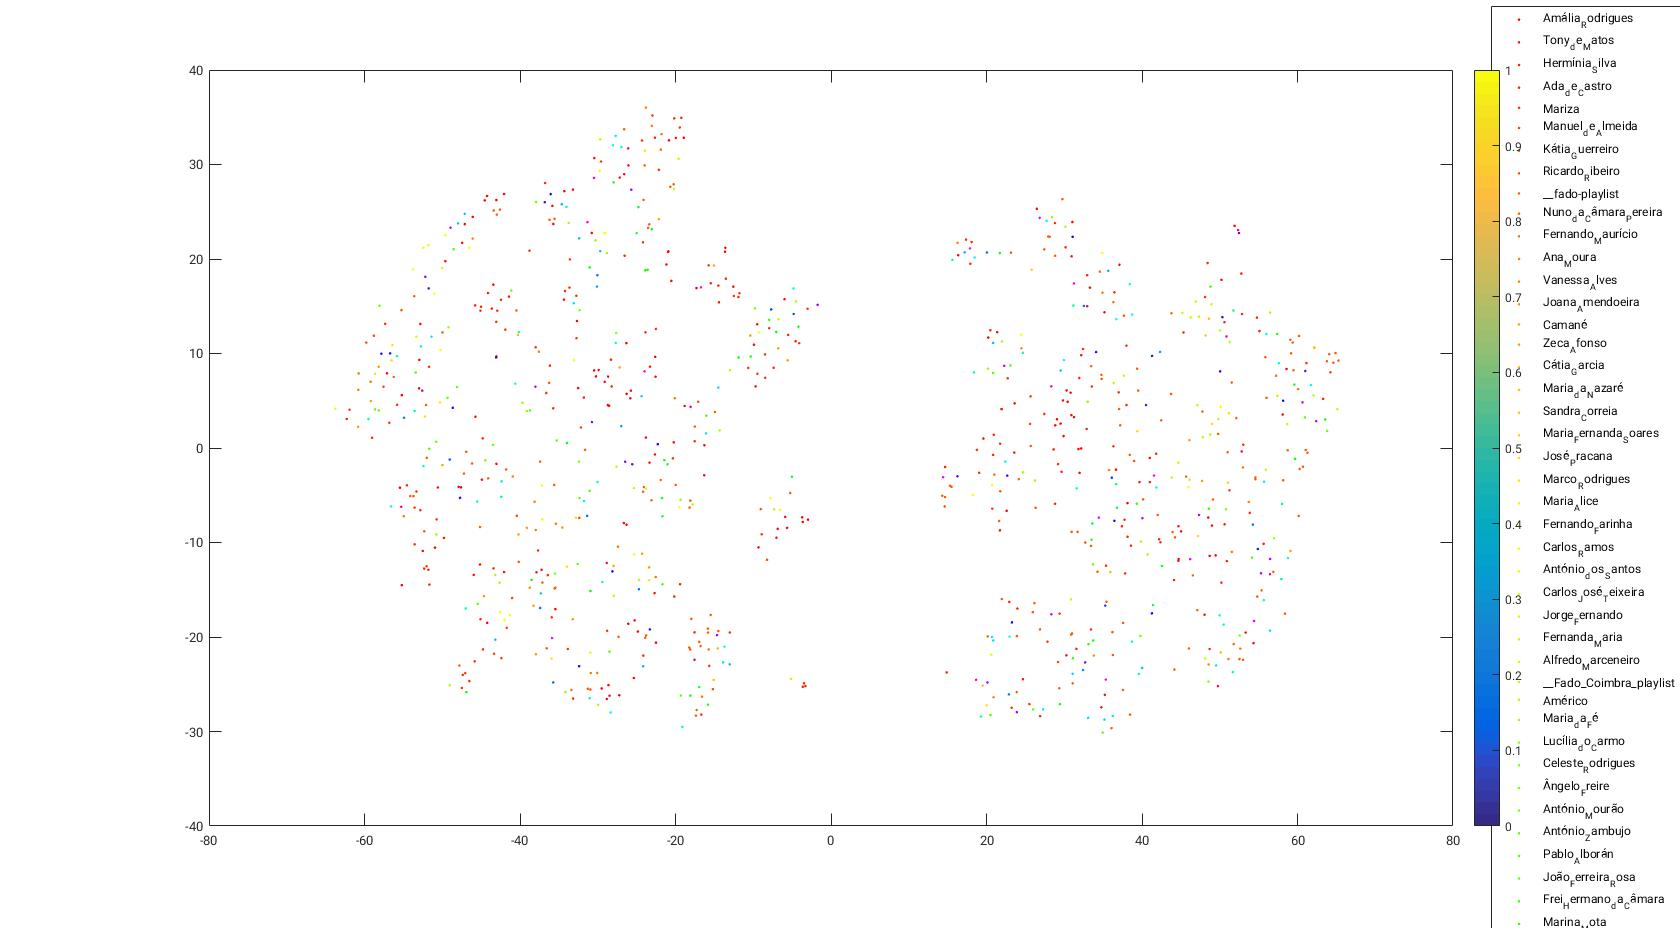
\includegraphics{Resources/phase0/Chroma/tsne/tsne_chroma.jpg}
\caption{tsne\_chroma\_2D}
\end{figure}

Imagem 1: TSNE às médias e variâncias das features Chroma de cada faixa
de música. Os pontos estão coloridos por artista. O tsne não revela
nenhum tipo de estrutura para além de dois grandes clusters.

    A ideia inicial era aplicar uma implementação de gaussian LDA - no
mirtools - a estas features contínuas para explorar possíveis tópicos
que se apresentassem. Nesta fase inicial estava a escrever scripts de
Bash e pequenos programas em C++ para tratar os dados, fazer
visualizações, e transformações necessárias, que - em retrospectiva -
consumiu muito tempo.

    \begin{figure}
\centering
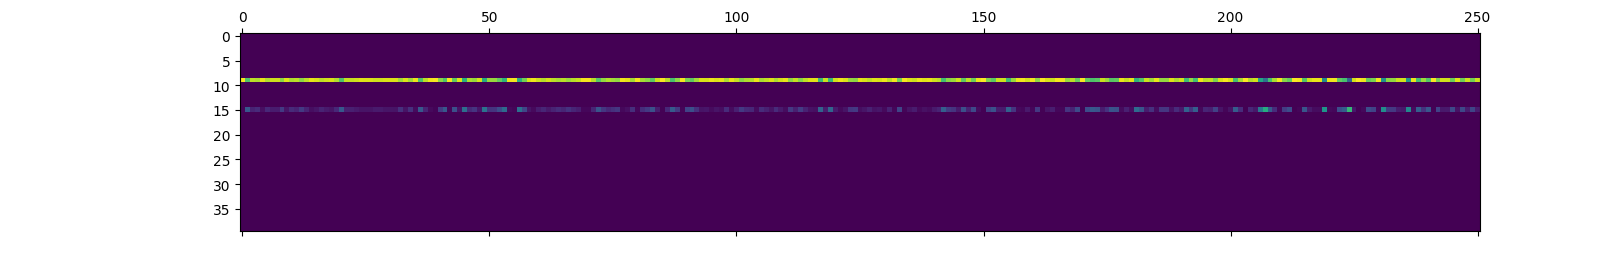
\includegraphics{Resources/phase0/Chroma/gLDA/glda_chroma_40_topics_40_iter.png}
\caption{glda\_chroma\_40\_topics}
\end{figure}

Imagem 2: Coeficientes dos tópicos em cada faixa

y: tópico - x: faixa

    Como é evidente, os resultados foram anómalos e foi passado bastante
tempo a rever scripts, aprender mais sobre e voltar a gerar as features
em MFCC e Chroma.

    \begin{Verbatim}[commandchars=\\\{\}]
{\color{incolor}In [{\color{incolor}4}]:} \PY{k}{def} \PY{n+nf}{invlogamplitude}\PY{p}{(}\PY{n}{S}\PY{p}{)}\PY{p}{:}
            \PY{l+s+sd}{\PYZdq{}\PYZdq{}\PYZdq{}librosa.logamplitude is actually 10\PYZus{}log10, so invert that.\PYZdq{}\PYZdq{}\PYZdq{}}
            \PY{k}{return} \PY{l+m+mf}{10.0}\PY{o}{*}\PY{o}{*}\PY{p}{(}\PY{n}{S}\PY{o}{/}\PY{l+m+mf}{10.0}\PY{p}{)}
        
        \PY{c+c1}{\PYZsh{} retorna nome de wavs em directório}
        \PY{k}{def} \PY{n+nf}{getWavNames}\PY{p}{(}\PY{n}{inputDir}\PY{p}{)}\PY{p}{:}
            \PY{n}{wavFileNames} \PY{o}{=} \PY{p}{[}\PY{n}{join}\PY{p}{(}\PY{n}{inputDir}\PY{p}{,} \PY{n}{f}\PY{p}{)} \PY{k}{for} \PY{n}{f} \PY{o+ow}{in} \PY{n}{listdir}\PY{p}{(}\PY{n}{inputDir}\PY{p}{)} \PY{k}{if} \PY{n}{isfile}\PY{p}{(}\PY{n}{join}\PY{p}{(}\PY{n}{inputDir}\PY{p}{,} \PY{n}{f}\PY{p}{)}\PY{p}{)} \PY{o+ow}{and} \PY{n}{f}\PY{p}{[}\PY{o}{\PYZhy{}}\PY{l+m+mi}{3}\PY{p}{:}\PY{p}{]}\PY{o}{==}\PY{l+s+s2}{\PYZdq{}}\PY{l+s+s2}{wav}\PY{l+s+s2}{\PYZdq{}}\PY{p}{]}
            \PY{c+c1}{\PYZsh{}usableIDs = [int(file[\PYZhy{}8:\PYZhy{}4]) for file in wavFileNames]}
        
            \PY{k}{return} \PY{n}{wavFileNames}
        
        \PY{c+c1}{\PYZsh{}n\PYZus{}mfcc: número de coeficientes desejados}
        \PY{c+c1}{\PYZsh{}nfft: comprimento para a fft, normalmente é a potência de 2 seguinte ao comprimento do maior sinal}
        \PY{n}{nfft} \PY{o}{=} \PY{l+m+mi}{256}
        \PY{k}{def} \PY{n+nf}{makeMFCC}\PY{p}{(}\PY{n}{inputDir}\PY{p}{,} \PY{n}{outputDir}\PY{p}{,} \PY{n}{n\PYZus{}mfcc}\PY{o}{=}\PY{l+m+mi}{20}\PY{p}{)}\PY{p}{:}
            \PY{n}{wavNames} \PY{o}{=} \PY{n}{getWavNames}\PY{p}{(}\PY{n}{inputDir}\PY{p}{)}
            
            \PY{k}{for} \PY{n}{filename} \PY{o+ow}{in} \PY{n}{wavNames}\PY{p}{:}
                \PY{c+c1}{\PYZsh{} load}
                \PY{n}{y}\PY{p}{,} \PY{n}{sr} \PY{o}{=} \PY{n}{librosa}\PY{o}{.}\PY{n}{load}\PY{p}{(}\PY{n}{filename}\PY{p}{)}
        
                \PY{c+c1}{\PYZsh{} calculate mfcc}
                \PY{n}{mfccs} \PY{o}{=} \PY{n}{librosa}\PY{o}{.}\PY{n}{feature}\PY{o}{.}\PY{n}{mfcc}\PY{p}{(}\PY{n}{y}\PY{p}{,} \PY{n}{sr}\PY{o}{=}\PY{n}{sr}\PY{p}{,} \PY{n}{n\PYZus{}mfcc}\PY{o}{=}\PY{n}{n\PYZus{}mfcc}\PY{p}{)}
                \PY{c+c1}{\PYZsh{}mfccName = filename[\PYZhy{}8:\PYZhy{}4] + \PYZdq{}\PYZus{}mfcc.csv\PYZdq{}}
                \PY{n}{mfccName} \PY{o}{=} \PY{n}{os}\PY{o}{.}\PY{n}{path}\PY{o}{.}\PY{n}{basename}\PY{p}{(}\PY{n}{filename}\PY{p}{)}\PY{p}{[}\PY{p}{:}\PY{o}{\PYZhy{}}\PY{l+m+mi}{4}\PY{p}{]} \PY{o}{+} \PY{l+s+s2}{\PYZdq{}}\PY{l+s+s2}{\PYZus{}mfcc.csv}\PY{l+s+s2}{\PYZdq{}}
                \PY{n}{saveDir} \PY{o}{=} \PY{n}{outputDir} \PY{o}{+} \PY{n}{mfccName}
                \PY{n}{mfccs} \PY{o}{=} \PY{n}{pd}\PY{o}{.}\PY{n}{DataFrame}\PY{p}{(}\PY{n}{mfccs}\PY{o}{.}\PY{n}{T}\PY{p}{)}
                \PY{n}{d}\PY{o}{.}\PY{n}{to\PYZus{}csv}\PY{p}{(}\PY{n}{saveDir}\PY{p}{)}
                \PY{n+nb}{print}\PY{p}{(}\PY{n}{filename} \PY{o}{+} \PY{l+s+s2}{\PYZdq{}}\PY{l+s+s2}{ }\PY{l+s+s2}{\PYZdq{}} \PY{o}{+} \PY{n+nb}{str}\PY{p}{(}\PY{n}{mfccs}\PY{o}{.}\PY{n}{shape}\PY{p}{)}\PY{p}{)}
                
        \PY{k}{def} \PY{n+nf}{makeChroma}\PY{p}{(}\PY{n}{inputDir}\PY{p}{,} \PY{n}{outputDir}\PY{p}{,} \PY{n}{nfft} \PY{o}{=} \PY{l+m+mi}{256}\PY{p}{)}\PY{p}{:}
            \PY{n}{wavNames} \PY{o}{=} \PY{n}{getWavNames}\PY{p}{(}\PY{n}{inputDir}\PY{p}{)}
            
            \PY{k}{for} \PY{n}{filename} \PY{o+ow}{in} \PY{n}{wavNames}\PY{p}{:}
                \PY{c+c1}{\PYZsh{}load}
                \PY{n}{y}\PY{p}{,} \PY{n}{sr} \PY{o}{=} \PY{n}{librosa}\PY{o}{.}\PY{n}{load}\PY{p}{(}\PY{n}{filename}\PY{p}{)}
                
                \PY{c+c1}{\PYZsh{}calculate chroma features}
                \PY{n}{chroma} \PY{o}{=} \PY{n}{librosa}\PY{o}{.}\PY{n}{feature}\PY{o}{.}\PY{n}{chroma\PYZus{}stft}\PY{p}{(}\PY{n}{y}\PY{o}{=}\PY{n}{y}\PY{p}{,} \PY{n}{sr}\PY{o}{=}\PY{n}{sr}\PY{p}{,} \PY{n}{n\PYZus{}fft} \PY{o}{=} \PY{n}{nfft}\PY{p}{,} \PY{n}{hop\PYZus{}length} \PY{o}{=} \PY{n+nb}{int}\PY{p}{(}\PY{n}{nfft}\PY{o}{/}\PY{l+m+mi}{2}\PY{p}{)}\PY{p}{)}
                \PY{n}{chromaName} \PY{o}{=} \PY{n}{os}\PY{o}{.}\PY{n}{path}\PY{o}{.}\PY{n}{basename}\PY{p}{(}\PY{n}{filename}\PY{p}{)}\PY{p}{[}\PY{p}{:}\PY{o}{\PYZhy{}}\PY{l+m+mi}{4}\PY{p}{]} \PY{o}{+} \PY{l+s+s2}{\PYZdq{}}\PY{l+s+s2}{\PYZus{}chroma.csv}\PY{l+s+s2}{\PYZdq{}}
                \PY{n}{saveDir} \PY{o}{=} \PY{n}{outputDir} \PY{o}{+} \PY{n}{chromaName}
                \PY{n}{chroma} \PY{o}{=} \PY{n}{pd}\PY{o}{.}\PY{n}{DataFrame}\PY{p}{(}\PY{n}{chroma}\PY{o}{.}\PY{n}{T}\PY{p}{)}
                \PY{n}{chroma}\PY{o}{.}\PY{n}{to\PYZus{}csv}\PY{p}{(}\PY{n}{saveDir}\PY{p}{)}
                \PY{n+nb}{print}\PY{p}{(}\PY{n}{filename} \PY{o}{+} \PY{l+s+s2}{\PYZdq{}}\PY{l+s+s2}{ }\PY{l+s+s2}{\PYZdq{}} \PY{o}{+} \PY{n+nb}{str}\PY{p}{(}\PY{n}{chroma}\PY{o}{.}\PY{n}{shape}\PY{p}{)}\PY{p}{)}
            
                
        \PY{c+c1}{\PYZsh{} Também consegui reconstruir sinal a partir das mfccs, mas o código não está a funcionar de momento.}
\end{Verbatim}


    \begin{Verbatim}[commandchars=\\\{\}]
{\color{incolor}In [{\color{incolor}5}]:} \PY{k+kn}{import} \PY{n+nn}{plotly}
        \PY{k+kn}{import} \PY{n+nn}{plotly}\PY{n+nn}{.}\PY{n+nn}{offline} \PY{k}{as} \PY{n+nn}{py}
        \PY{n}{plotly}\PY{o}{.}\PY{n}{offline}\PY{o}{.}\PY{n}{init\PYZus{}notebook\PYZus{}mode}\PY{p}{(}\PY{n}{connected}\PY{o}{=}\PY{k+kc}{True}\PY{p}{)}
        
        \PY{k+kn}{import} \PY{n+nn}{plotly}\PY{n+nn}{.}\PY{n+nn}{graph\PYZus{}objs} \PY{k}{as} \PY{n+nn}{go}
        \PY{k+kn}{import} \PY{n+nn}{plotly}\PY{n+nn}{.}\PY{n+nn}{figure\PYZus{}factory} \PY{k}{as} \PY{n+nn}{ff}
        \PY{k+kn}{import} \PY{n+nn}{colorlover} \PY{k}{as} \PY{n+nn}{cl}
\end{Verbatim}


    
    
    \begin{Verbatim}[commandchars=\\\{\}]
{\color{incolor}In [{\color{incolor}6}]:} \PY{n}{pd}\PY{o}{.}\PY{n}{options}\PY{o}{.}\PY{n}{display}\PY{o}{.}\PY{n}{max\PYZus{}columns} \PY{o}{=} \PY{l+m+mi}{50}
        \PY{n}{theta\PYZus{}glda\PYZus{}mirtools} \PY{o}{=} \PY{n}{pd}\PY{o}{.}\PY{n}{read\PYZus{}csv}\PY{p}{(}\PY{l+s+s2}{\PYZdq{}}\PY{l+s+s2}{/afs/l2f/home/frsc/Documents/ProjectosINESC/Fado/Full Report/Resources/phase1/Results/theta\PYZus{}gLDA\PYZus{}MFCC\PYZus{}mirtools.csv}\PY{l+s+s2}{\PYZdq{}} \PY{p}{,}\PY{n}{sep}\PY{o}{=}\PY{l+s+s2}{\PYZdq{}}\PY{l+s+s2}{ }\PY{l+s+s2}{\PYZdq{}}\PY{p}{,} \PY{n}{header}\PY{o}{=}\PY{k+kc}{None}\PY{p}{)}
        \PY{n}{theta\PYZus{}glda\PYZus{}mirtools} \PY{o}{=} \PY{n}{theta\PYZus{}glda\PYZus{}mirtools}\PY{o}{.}\PY{n}{T}
\end{Verbatim}


    \begin{Verbatim}[commandchars=\\\{\}]
{\color{incolor}In [{\color{incolor}7}]:} \PY{k}{def} \PY{n+nf}{tten}\PY{p}{(}\PY{n}{x}\PY{p}{)}\PY{p}{:}
            \PY{k}{return} \PY{n+nb}{int}\PY{p}{(}\PY{n}{x}\PY{o}{*}\PY{l+m+mi}{9}\PY{p}{)}
        
        \PY{c+c1}{\PYZsh{}theta samples x n\PYZus{}topics}
        \PY{k}{def} \PY{n+nf}{plotTheta}\PY{p}{(}\PY{n}{theta}\PY{p}{,} \PY{n}{num\PYZus{}songs}\PY{p}{)}\PY{p}{:}
            \PY{n}{colors} \PY{o}{=} \PY{n}{cl}\PY{o}{.}\PY{n}{scales}\PY{p}{[}\PY{l+s+s1}{\PYZsq{}}\PY{l+s+s1}{9}\PY{l+s+s1}{\PYZsq{}}\PY{p}{]}\PY{p}{[}\PY{l+s+s1}{\PYZsq{}}\PY{l+s+s1}{seq}\PY{l+s+s1}{\PYZsq{}}\PY{p}{]}\PY{p}{[}\PY{l+s+s1}{\PYZsq{}}\PY{l+s+s1}{Reds}\PY{l+s+s1}{\PYZsq{}}\PY{p}{]}
            \PY{n}{t} \PY{o}{=} \PY{n}{theta}
            \PY{n}{t}\PY{p}{[}\PY{l+s+s1}{\PYZsq{}}\PY{l+s+s1}{index\PYZus{}col}\PY{l+s+s1}{\PYZsq{}}\PY{p}{]} \PY{o}{=} \PY{n}{t}\PY{o}{.}\PY{n}{index}
            \PY{n}{t} \PY{o}{=} \PY{n}{t}\PY{p}{[}\PY{n}{t}\PY{o}{.}\PY{n}{columns}\PY{o}{.}\PY{n}{tolist}\PY{p}{(}\PY{p}{)}\PY{p}{[}\PY{o}{\PYZhy{}}\PY{l+m+mi}{1}\PY{p}{:}\PY{p}{]} \PY{o}{+} \PY{n}{t}\PY{o}{.}\PY{n}{columns}\PY{o}{.}\PY{n}{tolist}\PY{p}{(}\PY{p}{)}\PY{p}{[}\PY{p}{:}\PY{o}{\PYZhy{}}\PY{l+m+mi}{1}\PY{p}{]}\PY{p}{]}
            \PY{n}{col\PYZus{}n} \PY{o}{=} \PY{n+nb}{len}\PY{p}{(}\PY{n}{t}\PY{o}{.}\PY{n}{columns}\PY{p}{)}
            \PY{n}{row\PYZus{}n} \PY{o}{=} \PY{n+nb}{len}\PY{p}{(}\PY{n}{t}\PY{o}{.}\PY{n}{index}\PY{p}{)}
            \PY{n}{t\PYZus{}cols} \PY{o}{=} \PY{p}{[}\PY{n}{t}\PY{p}{[}\PY{n}{r}\PY{p}{]}\PY{o}{.}\PY{n}{apply}\PY{p}{(}\PY{n}{tten}\PY{p}{)}\PY{p}{[}\PY{p}{:}\PY{n}{num\PYZus{}songs}\PY{p}{]} \PY{k}{for} \PY{n}{r} \PY{o+ow}{in} \PY{n}{t}\PY{o}{.}\PY{n}{columns}\PY{p}{]}
            \PY{n}{t\PYZus{}cols\PYZus{}color} \PY{o}{=} \PY{n}{t\PYZus{}cols}
            \PY{n}{t\PYZus{}cols\PYZus{}color}\PY{p}{[}\PY{l+m+mi}{0}\PY{p}{]} \PY{o}{=} \PY{n}{t\PYZus{}cols\PYZus{}color}\PY{p}{[}\PY{l+m+mi}{1}\PY{p}{]}
            
        
            \PY{n}{trace0} \PY{o}{=} \PY{n}{go}\PY{o}{.}\PY{n}{Table}\PY{p}{(}
              \PY{n}{header} \PY{o}{=} \PY{n+nb}{dict}\PY{p}{(}
                \PY{n}{values} \PY{o}{=} \PY{n+nb}{list}\PY{p}{(}\PY{n+nb}{range}\PY{p}{(}\PY{n}{col\PYZus{}n}\PY{p}{)}\PY{p}{)}\PY{p}{,}
                \PY{n}{line} \PY{o}{=} \PY{n+nb}{dict}\PY{p}{(}\PY{n}{color} \PY{o}{=} \PY{l+s+s1}{\PYZsq{}}\PY{l+s+s1}{white}\PY{l+s+s1}{\PYZsq{}}\PY{p}{)}\PY{p}{,}
                \PY{n}{fill} \PY{o}{=} \PY{n+nb}{dict}\PY{p}{(}\PY{n}{color} \PY{o}{=} \PY{l+s+s1}{\PYZsq{}}\PY{l+s+s1}{white}\PY{l+s+s1}{\PYZsq{}}\PY{p}{)}\PY{p}{,}
                \PY{n}{align} \PY{o}{=} \PY{l+s+s1}{\PYZsq{}}\PY{l+s+s1}{center}\PY{l+s+s1}{\PYZsq{}}\PY{p}{,}
                \PY{n}{font} \PY{o}{=} \PY{n+nb}{dict}\PY{p}{(}\PY{n}{color} \PY{o}{=} \PY{l+s+s1}{\PYZsq{}}\PY{l+s+s1}{black}\PY{l+s+s1}{\PYZsq{}}\PY{p}{,} \PY{n}{size} \PY{o}{=} \PY{l+m+mi}{12}\PY{p}{)}
              \PY{p}{)}\PY{p}{,}
              \PY{n}{cells} \PY{o}{=} \PY{n+nb}{dict}\PY{p}{(}
                \PY{n}{values} \PY{o}{=} \PY{n}{t\PYZus{}cols}\PY{p}{,}
                \PY{n}{line} \PY{o}{=} \PY{n+nb}{dict}\PY{p}{(}\PY{n}{color} \PY{o}{=} \PY{p}{[}\PY{n}{np}\PY{o}{.}\PY{n}{array}\PY{p}{(}\PY{n}{colors}\PY{p}{)}\PY{p}{[}\PY{n}{np}\PY{o}{.}\PY{n}{array}\PY{p}{(}\PY{n}{c}\PY{p}{)}\PY{p}{]} \PY{k}{for} \PY{n}{c} \PY{o+ow}{in} \PY{n}{t\PYZus{}cols\PYZus{}color}\PY{p}{]}\PY{p}{)}\PY{p}{,}
                \PY{n}{fill} \PY{o}{=} \PY{n+nb}{dict}\PY{p}{(}\PY{n}{color} \PY{o}{=} \PY{p}{[}\PY{n}{np}\PY{o}{.}\PY{n}{array}\PY{p}{(}\PY{n}{colors}\PY{p}{)}\PY{p}{[}\PY{n}{np}\PY{o}{.}\PY{n}{array}\PY{p}{(}\PY{n}{c}\PY{p}{)}\PY{p}{]} \PY{k}{for} \PY{n}{c} \PY{o+ow}{in} \PY{n}{t\PYZus{}cols\PYZus{}color}\PY{p}{]}\PY{p}{)}\PY{p}{,}
                \PY{n}{align} \PY{o}{=} \PY{l+s+s1}{\PYZsq{}}\PY{l+s+s1}{center}\PY{l+s+s1}{\PYZsq{}}\PY{p}{,}
                \PY{n}{font} \PY{o}{=} \PY{n+nb}{dict}\PY{p}{(}\PY{n}{color} \PY{o}{=} \PY{l+s+s1}{\PYZsq{}}\PY{l+s+s1}{white}\PY{l+s+s1}{\PYZsq{}}\PY{p}{,} \PY{n}{size} \PY{o}{=} \PY{l+m+mi}{12}\PY{p}{)}
                \PY{p}{)}\PY{p}{)}
        
            \PY{n}{data} \PY{o}{=} \PY{p}{[}\PY{n}{trace0}\PY{p}{]}
        
            \PY{n}{py}\PY{o}{.}\PY{n}{iplot}\PY{p}{(}\PY{n}{data}\PY{p}{,} \PY{n}{filename} \PY{o}{=} \PY{l+s+s2}{\PYZdq{}}\PY{l+s+s2}{cell variable color}\PY{l+s+s2}{\PYZdq{}}\PY{p}{)}
\end{Verbatim}


    \begin{Verbatim}[commandchars=\\\{\}]
{\color{incolor}In [{\color{incolor}8}]:} \PY{n}{plotTheta}\PY{p}{(}\PY{n}{theta\PYZus{}glda\PYZus{}mirtools}\PY{p}{,}\PY{n}{theta\PYZus{}glda\PYZus{}mirtools}\PY{o}{.}\PY{n}{shape}\PY{p}{[}\PY{l+m+mi}{1}\PY{p}{]}\PY{p}{)}
\end{Verbatim}


    
    
    Figura 3: Valores são arredondamentos a inteiros para lhes poder
atribuir cores numa tabela do plotly.

    \begin{Verbatim}[commandchars=\\\{\}]
{\color{incolor}In [{\color{incolor}9}]:} \PY{n}{theta\PYZus{}glda\PYZus{}mirtools}\PY{o}{.}\PY{n}{describe}\PY{p}{(}\PY{p}{)}
\end{Verbatim}


\begin{Verbatim}[commandchars=\\\{\}]
{\color{outcolor}Out[{\color{outcolor}9}]:}                   0             1             2             3             4  \textbackslash{}
        count  7.410000e+02  7.410000e+02  7.410000e+02  7.410000e+02  7.410000e+02   
        mean   3.131209e-06  3.131209e-06  3.131209e-06  3.131209e-06  3.131209e-06   
        std    1.148827e-06  1.148827e-06  1.148827e-06  1.148827e-06  1.148827e-06   
        min    8.933996e-07  8.933996e-07  8.933996e-07  8.933996e-07  8.933996e-07   
        25\%    2.466213e-06  2.466213e-06  2.466213e-06  2.466213e-06  2.466213e-06   
        50\%    3.001921e-06  3.001921e-06  3.001921e-06  3.001921e-06  3.001921e-06   
        75\%    3.647505e-06  3.647505e-06  3.647505e-06  3.647505e-06  3.647505e-06   
        max    1.931994e-05  1.931994e-05  1.931994e-05  1.931994e-05  1.931994e-05   
        
                          5             6             7             8             9  \textbackslash{}
        count  7.410000e+02  7.410000e+02  7.410000e+02  7.410000e+02  7.410000e+02   
        mean   3.131209e-06  3.131209e-06  3.131209e-06  3.131209e-06  3.131209e-06   
        std    1.148827e-06  1.148827e-06  1.148827e-06  1.148827e-06  1.148827e-06   
        min    8.933996e-07  8.933996e-07  8.933996e-07  8.933996e-07  8.933996e-07   
        25\%    2.466213e-06  2.466213e-06  2.466213e-06  2.466213e-06  2.466213e-06   
        50\%    3.001921e-06  3.001921e-06  3.001921e-06  3.001921e-06  3.001921e-06   
        75\%    3.647505e-06  3.647505e-06  3.647505e-06  3.647505e-06  3.647505e-06   
        max    1.931994e-05  1.931994e-05  1.931994e-05  1.931994e-05  1.931994e-05   
        
                         10            11            12            13            14  \textbackslash{}
        count  7.410000e+02  7.410000e+02  7.410000e+02  7.410000e+02  7.410000e+02   
        mean   3.131209e-06  3.131209e-06  3.131209e-06  3.131209e-06  3.131209e-06   
        std    1.148827e-06  1.148827e-06  1.148827e-06  1.148827e-06  1.148827e-06   
        min    8.933996e-07  8.933996e-07  8.933996e-07  8.933996e-07  8.933996e-07   
        25\%    2.466213e-06  2.466213e-06  2.466213e-06  2.466213e-06  2.466213e-06   
        50\%    3.001921e-06  3.001921e-06  3.001921e-06  3.001921e-06  3.001921e-06   
        75\%    3.647505e-06  3.647505e-06  3.647505e-06  3.647505e-06  3.647505e-06   
        max    1.931994e-05  1.931994e-05  1.931994e-05  1.931994e-05  1.931994e-05   
        
                         15            16            17            18            19  \textbackslash{}
        count  7.410000e+02  7.410000e+02  7.410000e+02  7.410000e+02  7.410000e+02   
        mean   6.315357e-03  3.131209e-06  3.131209e-06  3.131209e-06  3.131209e-06   
        std    3.018236e-02  1.148827e-06  1.148827e-06  1.148827e-06  1.148827e-06   
        min    8.933996e-07  8.933996e-07  8.933996e-07  8.933996e-07  8.933996e-07   
        25\%    2.534469e-06  2.466213e-06  2.466213e-06  2.466213e-06  2.466213e-06   
        50\%    3.152585e-06  3.001921e-06  3.001921e-06  3.001921e-06  3.001921e-06   
        75\%    4.124051e-06  3.647505e-06  3.647505e-06  3.647505e-06  3.647505e-06   
        max    5.310067e-01  1.931994e-05  1.931994e-05  1.931994e-05  1.931994e-05   
        
                         20          21            22            23            24  \textbackslash{}
        count  7.410000e+02  741.000000  7.410000e+02  7.410000e+02  7.410000e+02   
        mean   3.131209e-06    0.993555  3.131209e-06  3.131209e-06  3.131209e-06   
        std    1.148827e-06    0.030208  1.148827e-06  1.148827e-06  1.148827e-06   
        min    8.933996e-07    0.468923  8.933996e-07  8.933996e-07  8.933996e-07   
        25\%    2.466213e-06    0.999839  2.466213e-06  2.466213e-06  2.466213e-06   
        50\%    3.001921e-06    0.999877  3.001921e-06  3.001921e-06  3.001921e-06   
        75\%    3.647505e-06    0.999901  3.647505e-06  3.647505e-06  3.647505e-06   
        max    1.931994e-05    0.999965  1.931994e-05  1.931994e-05  1.931994e-05   
        
                         25            26            27            28            29  \textbackslash{}
        count  7.410000e+02  7.410000e+02  7.410000e+02  7.410000e+02  7.410000e+02   
        mean   3.131209e-06  3.131209e-06  3.131209e-06  3.131209e-06  3.131209e-06   
        std    1.148827e-06  1.148827e-06  1.148827e-06  1.148827e-06  1.148827e-06   
        min    8.933996e-07  8.933996e-07  8.933996e-07  8.933996e-07  8.933996e-07   
        25\%    2.466213e-06  2.466213e-06  2.466213e-06  2.466213e-06  2.466213e-06   
        50\%    3.001921e-06  3.001921e-06  3.001921e-06  3.001921e-06  3.001921e-06   
        75\%    3.647505e-06  3.647505e-06  3.647505e-06  3.647505e-06  3.647505e-06   
        max    1.931994e-05  1.931994e-05  1.931994e-05  1.931994e-05  1.931994e-05   
        
                         30            31            32            33            34  \textbackslash{}
        count  7.410000e+02  7.410000e+02  7.410000e+02  7.410000e+02  7.410000e+02   
        mean   3.131209e-06  3.131209e-06  3.131209e-06  3.131209e-06  3.131209e-06   
        std    1.148827e-06  1.148827e-06  1.148827e-06  1.148827e-06  1.148827e-06   
        min    8.933996e-07  8.933996e-07  8.933996e-07  8.933996e-07  8.933996e-07   
        25\%    2.466213e-06  2.466213e-06  2.466213e-06  2.466213e-06  2.466213e-06   
        50\%    3.001921e-06  3.001921e-06  3.001921e-06  3.001921e-06  3.001921e-06   
        75\%    3.647505e-06  3.647505e-06  3.647505e-06  3.647505e-06  3.647505e-06   
        max    1.931994e-05  1.931994e-05  1.931994e-05  1.931994e-05  1.931994e-05   
        
                         35            36            37            38            39  \textbackslash{}
        count  7.410000e+02  7.410000e+02  7.410000e+02  7.410000e+02  7.410000e+02   
        mean   3.131209e-06  3.131209e-06  3.131209e-06  1.355196e-05  3.131209e-06   
        std    1.148827e-06  1.148827e-06  1.148827e-06  1.648472e-04  1.148827e-06   
        min    8.933996e-07  8.933996e-07  8.933996e-07  8.933996e-07  8.933996e-07   
        25\%    2.466213e-06  2.466213e-06  2.466213e-06  2.473044e-06  2.466213e-06   
        50\%    3.001921e-06  3.001921e-06  3.001921e-06  3.006253e-06  3.001921e-06   
        75\%    3.647505e-06  3.647505e-06  3.647505e-06  3.664614e-06  3.647505e-06   
        max    1.931994e-05  1.931994e-05  1.931994e-05  3.730113e-03  1.931994e-05   
        
                index\_col  
        count  741.000000  
        mean   370.000000  
        std    214.052564  
        min      0.000000  
        25\%    185.000000  
        50\%    370.000000  
        75\%    555.000000  
        max    740.000000  
\end{Verbatim}
            
    Como podemos observar, apenas os tópicos 15, 21, e 38 tomam valores com
ordem de magnitude superior a -5 para alguma canção. Isto sugere mau
funcionamento do gLDA já que a integridade dos dados foi assegurada pela
sua geração de raiz.

    Entretanto comecei a usar python, aprendi numpy, pandas, matplotlib, e
sklearn para acelerar o fluxo de trabalho. O refazer das features não
ajudou.

Sem solução em vista, escolhi discretizar as frames dos mfccs com kmeans
para lhes aplicar um LDA discreto. Isto funcionou melhor, com resultados
de aspecto natural, mas sem clusters óbvios. Antecipa-se que os
resultados encontrados reflictam regularidades na qualidade de gravação
mais do que aspectos musicais.

    \begin{Verbatim}[commandchars=\\\{\}]
{\color{incolor}In [{\color{incolor}7}]:} \PY{n}{wavDir} \PY{o}{=} \PY{l+s+s2}{\PYZdq{}}\PY{l+s+s2}{/ffs/tmp/frsc/fado/fado\PYZus{}init/wav/usable}\PY{l+s+s2}{\PYZdq{}}
        \PY{n}{mfccDir} \PY{o}{=} \PY{l+s+s2}{\PYZdq{}}\PY{l+s+s2}{/ffs/tmp/frsc/fado/fado\PYZus{}init/features3/mfcc/}\PY{l+s+s2}{\PYZdq{}}
        \PY{n}{chromaDir} \PY{o}{=} \PY{l+s+s2}{\PYZdq{}}\PY{l+s+s2}{/ffs/tmp/frsc/fado/fado\PYZus{}init/features2/chroma/}\PY{l+s+s2}{\PYZdq{}}
        \PY{n}{labelDir} \PY{o}{=} \PY{l+s+s2}{\PYZdq{}}\PY{l+s+s2}{/afs/l2f/home/frsc/Documents/ProjectosINESC/Fado/Full Report/Resources/phase1/labels.txt}\PY{l+s+s2}{\PYZdq{}}
        
        \PY{n}{N} \PY{o}{=} \PY{l+m+mi}{500}
        
        
        \PY{c+c1}{\PYZsh{}Directórios para teste com apenas 2 ficheiros de som}
        \PY{c+c1}{\PYZsh{}wavDir = \PYZdq{}/afs/l2f/home/frsc/Documents/ProjectosINESC/Fado/Full Report/Resources/isft/\PYZdq{}}
        \PY{c+c1}{\PYZsh{}mfccDir = \PYZdq{}/afs/l2f/home/frsc/Documents/ProjectosINESC/Fado/Full Report/Resources/isft/\PYZdq{}}
        \PY{c+c1}{\PYZsh{}chromaDir = \PYZdq{}/afs/l2f/home/frsc/Documents/ProjectosINESC/Fado/Full Report/Resources/isft/\PYZdq{}}
        \PY{c+c1}{\PYZsh{}labelDir = \PYZdq{}/afs/l2f/home/frsc/Documents/ProjectosINESC/Fado/Full Report/Resources/isft/label\PYZus{}example.txt\PYZdq{}}
        
        \PY{n}{featureDir}\PY{o}{=}\PY{n}{mfccDir}
\end{Verbatim}


    \begin{Verbatim}[commandchars=\\\{\}]
{\color{incolor}In [{\color{incolor}14}]:} \PY{c+c1}{\PYZsh{}featureTypeName: nome do tipo de feature, lowercase}
         \PY{c+c1}{\PYZsh{}idFromName: deduzir ID pelo nome qd tem formato \PYZdq{}0001\PYZus{}featuretype.csv\PYZdq{}}
         \PY{k}{def} \PY{n+nf}{buildSongsDF}\PY{p}{(}\PY{n}{featureDir}\PY{p}{,} \PY{n}{labelDir}\PY{p}{,} \PY{n}{featureTypeName}\PY{p}{,} \PY{n}{n\PYZus{}songs} \PY{o}{=} \PY{l+m+mi}{0}\PY{p}{,} \PY{n}{idFromName}\PY{o}{=}\PY{k+kc}{False}\PY{p}{)}\PY{p}{:}
             \PY{c+c1}{\PYZsh{} Load Labels}
             \PY{n}{labels\PYZus{}df} \PY{o}{=} \PY{n}{pd}\PY{o}{.}\PY{n}{read\PYZus{}csv}\PY{p}{(}\PY{n}{labelDir}\PY{p}{,} \PY{n}{delimiter} \PY{o}{=} \PY{l+s+s1}{\PYZsq{}}\PY{l+s+s1}{ \PYZhy{} }\PY{l+s+s1}{\PYZsq{}}\PY{p}{,} \PY{n}{header}\PY{o}{=}\PY{l+m+mi}{0}\PY{p}{,} \PY{n}{index\PYZus{}col} \PY{o}{=} \PY{l+m+mi}{0}\PY{p}{,} \PY{n}{dtype}\PY{o}{=}\PY{n+nb}{str}\PY{p}{)}
             
             \PY{c+c1}{\PYZsh{} Make filenames}
             \PY{n}{desiredSuffix} \PY{o}{=} \PY{n}{featureTypeName}\PY{o}{+}\PY{l+s+s2}{\PYZdq{}}\PY{l+s+s2}{.csv}\PY{l+s+s2}{\PYZdq{}}
             \PY{n}{files} \PY{o}{=} \PY{p}{[}\PY{n}{join}\PY{p}{(}\PY{n}{featureDir}\PY{p}{,} \PY{n}{f}\PY{p}{)} \PY{k}{for} \PY{n}{f} \PY{o+ow}{in} \PY{n}{listdir}\PY{p}{(}\PY{n}{featureDir}\PY{p}{)} \PY{k}{if} \PY{n}{isfile}\PY{p}{(}\PY{n}{join}\PY{p}{(}\PY{n}{featureDir}\PY{p}{,} \PY{n}{f}\PY{p}{)}\PY{p}{)} \PY{o+ow}{and} \PY{n}{f}\PY{o}{.}\PY{n}{endswith}\PY{p}{(}\PY{n}{desiredSuffix}\PY{p}{)}\PY{p}{]}
             
             \PY{c+c1}{\PYZsh{} Get IDs of songs to be loaded}
             \PY{n}{song\PYZus{}ids} \PY{o}{=} \PY{p}{[}\PY{p}{(}\PY{n}{os}\PY{o}{.}\PY{n}{path}\PY{o}{.}\PY{n}{basename}\PY{p}{(}\PY{n}{file}\PY{p}{)}\PY{p}{[}\PY{p}{:}\PY{o}{\PYZhy{}}\PY{n+nb}{len}\PY{p}{(}\PY{n}{desiredSuffix}\PY{p}{)}\PY{o}{\PYZhy{}}\PY{l+m+mi}{1}\PY{p}{]}\PY{p}{)} \PY{k}{for} \PY{n}{file} \PY{o+ow}{in} \PY{n}{files}\PY{p}{]}
             \PY{k}{if} \PY{n}{n\PYZus{}songs} \PY{o}{==} \PY{l+m+mi}{0}\PY{p}{:}
                 \PY{n}{song\PYZus{}n} \PY{o}{=} \PY{n+nb}{len}\PY{p}{(}\PY{n}{song\PYZus{}ids}\PY{p}{)}
             \PY{n}{song\PYZus{}n} \PY{o}{=} \PY{n}{n\PYZus{}songs}
         
             
             \PY{c+c1}{\PYZsh{} load songs}
             \PY{n}{song\PYZus{}list} \PY{o}{=} \PY{p}{[}\PY{k+kc}{None}\PY{p}{]} \PY{o}{*} \PY{n}{song\PYZus{}n}
             \PY{k}{for} \PY{n}{x} \PY{o+ow}{in} \PY{n+nb}{range}\PY{p}{(}\PY{n}{song\PYZus{}n}\PY{p}{)}\PY{p}{:}
                 \PY{n}{song\PYZus{}list}\PY{p}{[}\PY{n}{x}\PY{p}{]} \PY{o}{=} \PY{n}{pd}\PY{o}{.}\PY{n}{read\PYZus{}csv}\PY{p}{(}\PY{n}{files}\PY{p}{[}\PY{n}{x}\PY{p}{]}\PY{p}{,} \PY{n}{header}\PY{o}{=}\PY{k+kc}{None}\PY{p}{,} \PY{n}{index\PYZus{}col}\PY{o}{=}\PY{k+kc}{None}\PY{p}{)}
                 
             \PY{n}{song\PYZus{}ids} \PY{o}{=} \PY{n}{song\PYZus{}ids}\PY{p}{[}\PY{p}{:}\PY{n}{song\PYZus{}n}\PY{p}{]}
             \PY{n}{song\PYZus{}dict} \PY{o}{=} \PY{n+nb}{dict}\PY{p}{(}\PY{n+nb}{zip}\PY{p}{(}\PY{n}{song\PYZus{}ids}\PY{p}{,} \PY{n}{song\PYZus{}list}\PY{p}{)}\PY{p}{)}
         
             \PY{n}{songs\PYZus{}df} \PY{o}{=} \PY{n}{pd}\PY{o}{.}\PY{n}{concat}\PY{p}{(}\PY{n}{song\PYZus{}dict}\PY{p}{)}
             \PY{k}{return} \PY{n}{song\PYZus{}ids}\PY{p}{,} \PY{n}{songs\PYZus{}df}
\end{Verbatim}


    \begin{Verbatim}[commandchars=\\\{\}]
{\color{incolor}In [{\color{incolor}15}]:} \PY{n}{song\PYZus{}ids}\PY{p}{,} \PY{n}{songs\PYZus{}df} \PY{o}{=} \PY{n}{buildSongsDF}\PY{p}{(}\PY{n}{mfccDir}\PY{p}{,} \PY{n}{labelDir}\PY{p}{,} \PY{n}{n\PYZus{}songs}\PY{o}{=}\PY{n}{N}\PY{p}{,} \PY{n}{featureTypeName}\PY{o}{=}\PY{l+s+s2}{\PYZdq{}}\PY{l+s+s2}{mfcc}\PY{l+s+s2}{\PYZdq{}}\PY{p}{)}
\end{Verbatim}


    \begin{Verbatim}[commandchars=\\\{\}]
/afs/l2f.inesc-id.pt/home/frsc/virtualenv/lib/python3.4/site-packages/ipykernel\_launcher.py:5: ParserWarning:

Falling back to the 'python' engine because the 'c' engine does not support regex separators (separators > 1 char and different from '\textbackslash{}s+' are interpreted as regex); you can avoid this warning by specifying engine='python'.


    \end{Verbatim}

    \begin{Verbatim}[commandchars=\\\{\}]
{\color{incolor}In [{\color{incolor}16}]:} \PY{k}{def} \PY{n+nf}{discretizeContinuousFeatures}\PY{p}{(}\PY{n}{featureDir}\PY{p}{,} \PY{n}{labelDir}\PY{p}{,} \PY{n}{n\PYZus{}songs}\PY{o}{=}\PY{l+m+mi}{0}\PY{p}{,} \PY{n}{cluster\PYZus{}n}\PY{o}{=}\PY{l+m+mi}{100}\PY{p}{,} \PY{n}{featureTypeName}\PY{o}{=}\PY{l+s+s2}{\PYZdq{}}\PY{l+s+s2}{mfcc}\PY{l+s+s2}{\PYZdq{}}\PY{p}{)}\PY{p}{:}
             
             \PY{c+c1}{\PYZsh{}KMeans}
             \PY{n}{song\PYZus{}ids}\PY{p}{,} \PY{n}{songs\PYZus{}df} \PY{o}{=} \PY{n}{buildSongsDF}\PY{p}{(}\PY{n}{featureDir}\PY{p}{,} \PY{n}{labelDir}\PY{p}{,} \PY{n}{n\PYZus{}songs} \PY{o}{=} \PY{n}{n\PYZus{}songs}\PY{p}{,} \PY{n}{featureTypeName} \PY{o}{=} \PY{n}{featureTypeName}\PY{p}{)}
             \PY{n}{songs\PYZus{}df\PYZus{}scaled} \PY{o}{=} \PY{n}{pd}\PY{o}{.}\PY{n}{DataFrame}\PY{p}{(}\PY{n}{preprocessing}\PY{o}{.}\PY{n}{scale}\PY{p}{(}\PY{n}{songs\PYZus{}df}\PY{p}{)}\PY{p}{)}
             \PY{n}{song\PYZus{}n} \PY{o}{=} \PY{n+nb}{len}\PY{p}{(}\PY{n}{song\PYZus{}ids}\PY{p}{)}
             
             \PY{n}{X\PYZus{}NEW} \PY{o}{=} \PY{n}{MiniBatchKMeans}\PY{p}{(}\PY{n}{n\PYZus{}clusters}\PY{o}{=}\PY{n}{cluster\PYZus{}n}\PY{p}{,} \PY{n}{random\PYZus{}state}\PY{o}{=}\PY{l+m+mi}{0}\PY{p}{)}\PY{o}{.}\PY{n}{fit\PYZus{}predict}\PY{p}{(}\PY{n}{songs\PYZus{}df\PYZus{}scaled}\PY{p}{)}
             \PY{n}{x\PYZus{}df} \PY{o}{=} \PY{n}{pd}\PY{o}{.}\PY{n}{DataFrame}\PY{p}{(}\PY{n}{X\PYZus{}NEW}\PY{p}{)}
             \PY{n}{x\PYZus{}df}\PY{o}{.}\PY{n}{groupby}\PY{p}{(}\PY{l+m+mi}{0}\PY{p}{)}\PY{o}{.}\PY{n}{size}\PY{p}{(}\PY{p}{)}
         
             \PY{c+c1}{\PYZsh{} Reconstruir Canções com isto}
             \PY{n}{song\PYZus{}lens} \PY{o}{=} \PY{p}{[}\PY{n+nb}{len}\PY{p}{(}\PY{n}{songs\PYZus{}df}\PY{o}{.}\PY{n}{loc}\PY{p}{[}\PY{n}{x}\PY{p}{]}\PY{p}{)} \PY{k}{for} \PY{n}{x} \PY{o+ow}{in} \PY{n}{song\PYZus{}ids}\PY{p}{]}
             
             \PY{n}{discrete\PYZus{}songs} \PY{o}{=} \PY{p}{[}\PY{k+kc}{None}\PY{p}{]}\PY{o}{*}\PY{n}{song\PYZus{}n}
             \PY{n}{high} \PY{o}{=} \PY{l+m+mi}{0}
             \PY{n}{low} \PY{o}{=} \PY{l+m+mi}{0}
             \PY{k}{for} \PY{n}{i} \PY{o+ow}{in} \PY{n+nb}{range}\PY{p}{(}\PY{n}{song\PYZus{}n}\PY{p}{)}\PY{p}{:}
                 \PY{n}{high} \PY{o}{+}\PY{o}{=} \PY{n}{song\PYZus{}lens}\PY{p}{[}\PY{n}{i}\PY{p}{]}
                 \PY{n}{discrete\PYZus{}songs}\PY{p}{[}\PY{n}{i}\PY{p}{]} \PY{o}{=} \PY{n}{X\PYZus{}NEW}\PY{p}{[}\PY{n}{low}\PY{p}{:}\PY{n}{high}\PY{p}{]}
                 \PY{n}{low} \PY{o}{=} \PY{n}{high}
                 
             \PY{n}{kmeansDir} \PY{o}{=} \PY{n}{featureDir} \PY{o}{+} \PY{l+s+s2}{\PYZdq{}}\PY{l+s+s2}{meta/fadoKmeans.csv}\PY{l+s+s2}{\PYZdq{}}
             
             \PY{n}{x\PYZus{}df}\PY{o}{.}\PY{n}{to\PYZus{}csv}\PY{p}{(}\PY{n}{path\PYZus{}or\PYZus{}buf}\PY{o}{=}\PY{n}{kmeansDir}\PY{p}{,} \PY{n}{index}\PY{o}{=}\PY{k+kc}{False}\PY{p}{)}
         
             \PY{n+nb}{print}\PY{p}{(}\PY{l+s+s2}{\PYZdq{}}\PY{l+s+s2}{Document lengths:}\PY{l+s+se}{\PYZbs{}n}\PY{l+s+s2}{\PYZdq{}}\PY{p}{)}
             \PY{k}{for} \PY{n}{i} \PY{o+ow}{in} \PY{n+nb}{range}\PY{p}{(}\PY{n}{song\PYZus{}n}\PY{p}{)}\PY{p}{:}
                 \PY{n+nb}{print}\PY{p}{(}\PY{l+s+s2}{\PYZdq{}}\PY{l+s+s2}{Song }\PY{l+s+si}{\PYZob{}0\PYZcb{}}\PY{l+s+s2}{: }\PY{l+s+si}{\PYZob{}1\PYZcb{}}\PY{l+s+s2}{\PYZdq{}}\PY{o}{.}\PY{n}{format}\PY{p}{(}\PY{n}{song\PYZus{}ids}\PY{p}{[}\PY{n}{i}\PY{p}{]}\PY{p}{,}\PY{n+nb}{len}\PY{p}{(}\PY{n}{discrete\PYZus{}songs}\PY{p}{[}\PY{n}{i}\PY{p}{]}\PY{p}{)}\PY{p}{)}\PY{p}{)}
             \PY{k}{return} \PY{n}{x\PYZus{}df}\PY{p}{,} \PY{n}{discrete\PYZus{}songs}
\end{Verbatim}


    \begin{Verbatim}[commandchars=\\\{\}]
{\color{incolor}In [{\color{incolor}165}]:} \PY{n}{x\PYZus{}df}\PY{p}{,} \PY{n}{discrete\PYZus{}songs} \PY{o}{=} \PY{n}{discretizeContinuousFeatures}\PY{p}{(}\PY{n}{mfccDir}\PY{p}{,} \PY{n}{labelDir}\PY{p}{,} \PY{n}{n\PYZus{}songs} \PY{o}{=} \PY{n}{N}\PY{p}{,} \PY{n}{featureTypeName}\PY{o}{=}\PY{l+s+s2}{\PYZdq{}}\PY{l+s+s2}{mfcc}\PY{l+s+s2}{\PYZdq{}}\PY{p}{)}
\end{Verbatim}


    \begin{Verbatim}[commandchars=\\\{\}]
/afs/l2f.inesc-id.pt/home/frsc/virtualenv/lib/python3.4/site-packages/ipykernel\_launcher.py:5: ParserWarning:

Falling back to the 'python' engine because the 'c' engine does not support regex separators (separators > 1 char and different from '\textbackslash{}s+' are interpreted as regex); you can avoid this warning by specifying engine='python'.


    \end{Verbatim}

    \begin{Verbatim}[commandchars=\\\{\}]
Document lengths:

Song 0001: 5430
Song 0054: 6794
Song 0055: 13523
Song 0057: 6766
Song 0058: 8043
Song 0059: 9057
Song 0060: 7627
Song 0061: 8810
Song 0062: 6993
Song 0063: 6787
Song 0064: 6498
Song 0065: 6215
Song 0066: 6857
Song 0067: 7623
Song 0068: 6206
Song 0069: 7363
Song 0070: 7663
Song 0071: 6379
Song 0073: 11147
Song 0075: 9885
Song 0076: 9142
Song 0077: 6673
Song 0078: 11707
Song 0079: 11051
Song 0080: 8835
Song 0081: 7400
Song 0082: 12859
Song 0083: 10048
Song 0084: 11111
Song 0085: 8312
Song 0086: 8544
Song 0087: 12857
Song 0088: 8021
Song 0089: 5781
Song 0090: 6599
Song 0091: 8237
Song 0094: 8268
Song 0095: 7197
Song 0096: 14078
Song 0097: 6978
Song 0098: 6281
Song 0099: 9863
Song 0100: 7812
Song 0102: 6169
Song 0104: 6905
Song 0105: 7499
Song 0106: 8535
Song 0107: 9233
Song 0109: 8177
Song 0110: 6327
Song 0111: 6739
Song 0112: 5518
Song 0113: 6359
Song 0114: 6743
Song 0115: 7470
Song 0116: 6552
Song 0117: 8410
Song 0118: 7959
Song 0119: 10699
Song 0121: 8748
Song 0122: 12872
Song 0123: 7077
Song 0124: 7905
Song 0125: 15395
Song 0126: 10014
Song 0127: 9423
Song 0128: 6628
Song 0130: 5623
Song 0131: 10167
Song 0132: 9043
Song 0133: 7205
Song 0134: 8659
Song 0135: 5699
Song 0136: 5818
Song 0137: 7073
Song 0138: 5873
Song 0139: 10731
Song 0140: 9019
Song 0141: 9222
Song 0142: 8875
Song 0143: 9265
Song 0144: 9172
Song 0145: 6673
Song 0146: 13905
Song 0147: 13185
Song 0148: 9487
Song 0149: 7541
Song 0150: 10241
Song 0152: 7327
Song 0153: 9759
Song 0154: 9341
Song 0157: 9487
Song 0158: 9767
Song 0159: 7171
Song 0160: 6841
Song 0161: 5663
Song 0162: 6289
Song 0163: 6839
Song 0164: 8709
Song 0165: 6044
Song 0166: 5581
Song 0167: 12927
Song 0168: 12899
Song 0169: 5598
Song 0170: 5265
Song 0171: 6294
Song 0172: 18066
Song 0174: 9165
Song 0175: 9144
Song 0176: 5699
Song 0177: 7690
Song 0179: 11190
Song 0180: 5980
Song 0181: 12278
Song 0182: 9245
Song 0184: 13661
Song 0186: 6544
Song 0188: 8230
Song 0189: 10933
Song 0190: 13107
Song 0191: 13202
Song 0192: 14308
Song 0194: 12470
Song 0195: 7218
Song 0196: 7929
Song 0197: 9434
Song 0198: 7236
Song 0199: 6289
Song 0200: 10132
Song 0201: 7509
Song 0202: 10399
Song 0203: 6625
Song 0204: 11014
Song 0205: 11470
Song 0206: 7544
Song 0207: 9904
Song 0208: 15068
Song 0209: 18877
Song 0210: 10511
Song 0211: 7015
Song 0212: 3796
Song 0213: 13513
Song 0214: 10418
Song 0215: 9872
Song 0216: 10554
Song 0217: 8096
Song 0219: 10108
Song 0220: 9712
Song 0221: 10564
Song 0222: 13176
Song 0224: 10172
Song 0225: 12182
Song 0226: 10850
Song 0227: 9893
Song 0229: 8113
Song 0230: 8368
Song 0231: 7567
Song 0232: 3662
Song 0233: 9873
Song 0234: 12071
Song 0235: 17118
Song 0236: 14687
Song 0237: 13183
Song 0238: 10665
Song 0239: 8173
Song 0240: 11708
Song 0241: 7938
Song 0242: 6906
Song 0243: 9175
Song 0244: 11102
Song 0245: 18024
Song 0246: 9091
Song 0247: 8912
Song 0248: 7086
Song 0249: 14193
Song 0250: 6527
Song 0251: 11471
Song 0252: 9323
Song 0253: 10364
Song 0254: 8649
Song 0255: 9459
Song 0256: 8561
Song 0258: 7097
Song 0260: 20564
Song 0261: 4439
Song 0262: 6763
Song 0263: 10765
Song 0264: 10052
Song 0265: 9316
Song 0266: 14049
Song 0267: 10151
Song 0268: 10397
Song 0269: 8989
Song 0271: 10605
Song 0273: 11357
Song 0274: 10984
Song 0275: 6928
Song 0276: 11609
Song 0277: 10769
Song 0280: 7498
Song 0497: 8153
Song 0498: 9500
Song 0499: 5861
Song 0500: 15534
Song 0502: 6461
Song 0503: 6035
Song 0504: 13203
Song 0505: 13185
Song 0506: 9731
Song 0507: 7719
Song 0508: 17029
Song 0509: 4941
Song 0510: 10999
Song 0511: 3443
Song 0512: 11418
Song 0513: 7145
Song 0514: 14617
Song 0515: 5464
Song 0517: 9495
Song 0518: 5571
Song 0519: 7269
Song 0520: 9484
Song 0521: 8353
Song 0522: 7141
Song 0523: 10665
Song 0524: 7785
Song 0525: 10511
Song 0526: 4787
Song 0527: 14149
Song 0528: 7737
Song 0529: 6367
Song 0530: 7663
Song 0531: 11805
Song 0532: 7653
Song 0533: 5028
Song 0534: 7825
Song 0535: 5891
Song 0536: 11891
Song 0537: 9278
Song 0538: 8020
Song 0539: 7534
Song 0540: 5160
Song 0541: 7210
Song 0542: 7425
Song 0543: 11589
Song 0544: 10915
Song 0546: 10435
Song 0547: 8948
Song 0548: 8327
Song 0549: 8290
Song 0550: 9691
Song 0551: 12310
Song 0552: 7096
Song 0553: 8131
Song 0554: 9066
Song 0555: 9845
Song 0556: 8809
Song 0557: 14772
Song 0558: 8076
Song 0559: 8657
Song 0560: 12687
Song 0561: 8467
Song 0562: 10790
Song 0563: 11935
Song 0564: 9908
Song 0565: 4157
Song 0566: 10465
Song 0567: 13933
Song 0568: 6199
Song 0569: 7582
Song 0570: 10360
Song 0572: 9215
Song 0573: 12722
Song 0574: 10038
Song 0575: 6731
Song 0576: 8108
Song 0577: 6843
Song 0578: 6283
Song 0580: 7915
Song 0581: 5673
Song 0582: 7821
Song 0583: 7880
Song 0584: 7421
Song 0585: 9221
Song 0586: 8757
Song 0587: 9871
Song 0588: 7325
Song 0589: 7879
Song 0591: 11635
Song 0592: 10167
Song 0593: 5728
Song 0594: 9145
Song 0595: 3795
Song 0596: 5420
Song 0597: 16971
Song 0598: 9244
Song 0599: 14471
Song 0600: 18162
Song 0601: 21910
Song 0604: 12417
Song 0605: 5469
Song 0606: 13759
Song 0607: 14749
Song 0608: 9926
Song 0609: 11365
Song 0610: 8897
Song 0611: 6130
Song 0612: 9555
Song 0613: 9078
Song 0614: 8884
Song 0615: 8499
Song 0616: 9261
Song 0617: 11375
Song 0618: 12206
Song 0619: 9060
Song 0621: 7795
Song 0622: 8613
Song 0623: 10050
Song 0624: 5792
Song 0625: 10243
Song 0626: 11471
Song 0627: 5885
Song 0628: 6795
Song 0629: 6701
Song 0630: 6795
Song 0631: 9167
Song 0632: 7591
Song 0633: 9681
Song 0634: 6885
Song 0635: 6599
Song 0636: 7002
Song 0637: 6421
Song 0638: 9603
Song 0639: 8787
Song 0640: 7607
Song 0641: 18453
Song 0642: 4567
Song 0643: 9457
Song 0644: 5043
Song 0645: 6562
Song 0646: 5905
Song 0647: 6728
Song 0648: 4265
Song 0649: 6980
Song 0651: 3238
Song 0652: 10384
Song 0653: 11374
Song 0654: 8975
Song 0656: 12534
Song 0657: 12242
Song 0659: 13185
Song 0660: 9644
Song 0661: 6119
Song 0662: 8821
Song 0663: 6963
Song 0664: 6061
Song 0665: 11725
Song 0666: 7979
Song 0667: 5763
Song 0668: 5507
Song 0669: 15857
Song 0670: 9004
Song 0671: 17671
Song 0672: 4714
Song 0673: 8893
Song 0674: 9293
Song 0675: 8561
Song 0676: 7247
Song 0677: 5631
Song 0678: 10667
Song 0679: 7724
Song 0680: 20414
Song 0681: 5219
Song 0682: 7731
Song 0683: 7883
Song 0684: 8228
Song 0685: 11582
Song 0686: 7879
Song 0687: 7648
Song 0688: 8186
Song 0689: 8303
Song 0690: 12553
Song 0692: 10017
Song 0693: 4530
Song 0694: 10187
Song 0695: 8749
Song 0696: 11421
Song 0697: 8384
Song 0698: 8065
Song 0699: 8220
Song 0700: 5603
Song 0701: 7919
Song 0702: 10136
Song 0703: 9841
Song 0704: 6502
Song 0706: 4225
Song 0712: 6551
Song 0713: 9601
Song 0714: 5837
Song 0716: 5792
Song 0717: 6525
Song 0718: 8622
Song 0719: 6842
Song 0722: 7541
Song 0724: 7637
Song 0726: 15761
Song 0728: 7775
Song 0732: 6665
Song 0733: 9183
Song 0736: 6427
Song 0737: 7257
Song 0739: 9529
Song 0740: 6634
Song 0741: 8177
Song 0742: 7497
Song 0744: 7937
Song 0748: 5361
Song 0751: 7840
Song 0752: 7064
Song 0753: 10825
Song 0754: 1293
Song 0755: 7625
Song 0759: 5681
Song 0760: 4197
Song 0763: 9664
Song 0766: 6483
Song 0767: 8329
Song 0769: 4653
Song 0770: 7997
Song 0772: 3154
Song 0773: 13709
Song 0774: 11692
Song 0775: 9628
Song 0776: 8259
Song 0778: 7829
Song 0781: 13266
Song 0782: 11018
Song 0783: 8126
Song 0784: 10323
Song 0786: 9535
Song 0787: 17534
Song 0788: 9705
Song 0790: 6011
Song 0792: 10984
Song 0793: 6188
Song 0794: 9261
Song 0795: 10315
Song 0796: 3147
Song 0797: 6489
Song 0799: 16997
Song 0800: 5249
Song 0801: 5686
Song 0802: 6505
Song 0803: 6204
Song 0804: 6928
Song 0805: 6741
Song 0806: 8618
Song 0808: 5470
Song 0809: 9132
Song 0810: 9273
Song 0811: 9293
Song 0812: 7484
Song 0813: 7153
Song 0814: 7363
Song 0815: 10549
Song 0816: 10251
Song 0817: 9591
Song 0818: 8865
Song 0819: 12845
Song 0820: 6976
Song 0821: 9865
Song 0822: 4931
Song 0823: 7595
Song 0824: 9179
Song 0825: 5939
Song 0826: 5387
Song 0827: 9065
Song 0828: 7513
Song 0829: 10516
Song 0830: 8443
Song 0831: 7279
Song 0832: 12192
Song 0833: 6519
Song 0834: 7446
Song 0835: 6033
Song 0836: 4636
Song 0837: 19504
Song 0838: 8073
Song 0839: 19276
Song 0840: 8893
Song 0841: 9544
Song 0842: 8844
Song 0843: 10199
Song 0844: 10079
Song 0845: 9887
Song 0846: 9322
Song 0847: 7167
Song 0848: 6328
Song 0849: 5516
Song 0850: 6615

    \end{Verbatim}

    \begin{Verbatim}[commandchars=\\\{\}]
{\color{incolor}In [{\color{incolor}166}]:} \PY{c+c1}{\PYZsh{}Frequências de cada \PYZdq{}palavra\PYZdq{}}
          \PY{n}{x\PYZus{}df}\PY{p}{[}\PY{l+m+mi}{0}\PY{p}{]}\PY{o}{.}\PY{n}{value\PYZus{}counts}\PY{p}{(}\PY{p}{)}
\end{Verbatim}


\begin{Verbatim}[commandchars=\\\{\}]
{\color{outcolor}Out[{\color{outcolor}166}]:} 24    96205
          48    88591
          19    88189
          35    76366
          89    74882
          2     74149
          65    72416
          45    71858
          79    71769
          5     71682
          21    71646
          13    70372
          40    69576
          36    69069
          15    67124
          17    66212
          59    65080
          53    64741
          87    63338
          26    63027
          78    61963
          8     60807
          46    60695
          37    60284
          50    59072
          63    58873
          1     58723
          54    58097
          29    57749
          92    57003
                {\ldots}  
          68    32633
          91    32529
          56    31938
          55    31690
          51    31228
          32    30615
          30    30604
          75    29775
          7     29466
          73    29041
          16    27884
          96    27754
          41    26396
          72    25327
          44    24578
          95    24110
          85    23954
          20    23810
          28    23309
          81    22470
          97    21507
          71    21328
          12    21168
          90    20319
          42    19402
          70    17500
          74    17162
          84    14178
          93    13184
          62    10938
          Name: 0, Length: 100, dtype: int64
\end{Verbatim}
            
    \begin{Verbatim}[commandchars=\\\{\}]
{\color{incolor}In [{\color{incolor}8}]:} \PY{c+c1}{\PYZsh{} Fazer document\PYZhy{}word matrix}
        \PY{k+kn}{from} \PY{n+nn}{sklearn}\PY{n+nn}{.}\PY{n+nn}{feature\PYZus{}extraction} \PY{k}{import} \PY{n}{DictVectorizer}
        \PY{k+kn}{from} \PY{n+nn}{collections} \PY{k}{import} \PY{n}{Counter}\PY{p}{,} \PY{n}{OrderedDict}
        
        \PY{k}{def} \PY{n+nf}{makeDocWordMatrix}\PY{p}{(}\PY{n}{mfccDir}\PY{p}{,} \PY{n}{discrete\PYZus{}songs}\PY{p}{)}\PY{p}{:}
        
            \PY{n}{vectorizer} \PY{o}{=} \PY{n}{DictVectorizer}\PY{p}{(}\PY{p}{)}
            \PY{c+c1}{\PYZsh{} discover corpus and vectorize file word frequencies in a single pass}
            \PY{n}{dwm} \PY{o}{=} \PY{n}{vectorizer}\PY{o}{.}\PY{n}{fit\PYZus{}transform}\PY{p}{(}\PY{n}{Counter}\PY{p}{(}\PY{n}{f}\PY{p}{)} \PY{k}{for} \PY{n}{f} \PY{o+ow}{in} \PY{p}{(}\PY{n}{discrete\PYZus{}songs}\PY{p}{)}\PY{p}{)}
            \PY{c+c1}{\PYZsh{}dwm = pd.DataFrame(dwm)}
            \PY{c+c1}{\PYZsh{}dwm.to\PYZus{}csv(mfccDir+\PYZdq{}meta/DWM.csv\PYZdq{})}
            \PY{k}{return} \PY{n}{dwm}
\end{Verbatim}


    \begin{Verbatim}[commandchars=\\\{\}]
{\color{incolor}In [{\color{incolor}168}]:} \PY{n}{dwm} \PY{o}{=} \PY{n}{makeDocWordMatrix}\PY{p}{(}\PY{n}{mfccDir}\PY{p}{,} \PY{n}{discrete\PYZus{}songs}\PY{p}{)}
\end{Verbatim}


    \begin{Verbatim}[commandchars=\\\{\}]
{\color{incolor}In [{\color{incolor}9}]:} \PY{k+kn}{from} \PY{n+nn}{sklearn}\PY{n+nn}{.}\PY{n+nn}{decomposition} \PY{k}{import} \PY{n}{LatentDirichletAllocation}
        
        \PY{k}{def} \PY{n+nf}{runLDA}\PY{p}{(}\PY{n}{dwm}\PY{p}{,} \PY{n}{outputPath}\PY{p}{)}\PY{p}{:}
            \PY{n}{lda} \PY{o}{=} \PY{n}{LatentDirichletAllocation}\PY{p}{(}\PY{n}{n\PYZus{}components}\PY{o}{=}\PY{l+m+mi}{40}\PY{p}{,} \PY{n}{random\PYZus{}state}\PY{o}{=}\PY{l+m+mi}{0}\PY{p}{,} \PY{n}{evaluate\PYZus{}every}\PY{o}{=}\PY{l+m+mi}{10}\PY{p}{)}
            \PY{n}{theta} \PY{o}{=} \PY{n}{lda}\PY{o}{.}\PY{n}{fit\PYZus{}transform}\PY{p}{(}\PY{n}{dwm}\PY{p}{)}
        
            \PY{n}{theta} \PY{o}{=} \PY{n}{pd}\PY{o}{.}\PY{n}{DataFrame}\PY{p}{(}\PY{n}{theta}\PY{p}{)}
            \PY{n}{theta}\PY{o}{.}\PY{n}{describe}\PY{p}{(}\PY{p}{)}
            \PY{n}{theta}\PY{o}{.}\PY{n}{to\PYZus{}csv}\PY{p}{(}\PY{n}{outputPath}\PY{p}{)}
            \PY{k}{return} \PY{n}{theta}
            
\end{Verbatim}


    \begin{Verbatim}[commandchars=\\\{\}]
{\color{incolor}In [{\color{incolor}169}]:} \PY{n}{theta} \PY{o}{=} \PY{n}{runLDA}\PY{p}{(}\PY{n}{dwm}\PY{p}{,} \PY{n}{mfccDir}\PY{o}{+}\PY{l+s+s2}{\PYZdq{}}\PY{l+s+s2}{meta/LDAtheta.csv}\PY{l+s+s2}{\PYZdq{}}\PY{p}{)}
          \PY{n}{theta}\PY{o}{.}\PY{n}{to\PYZus{}csv}\PY{p}{(}\PY{l+s+s2}{\PYZdq{}}\PY{l+s+s2}{test\PYZus{}theta.csv}\PY{l+s+s2}{\PYZdq{}}\PY{p}{)}
\end{Verbatim}


    \begin{Verbatim}[commandchars=\\\{\}]
/afs/l2f.inesc-id.pt/home/frsc/virtualenv/lib/python3.4/site-packages/sklearn/decomposition/online\_lda.py:536: DeprecationWarning:

The default value for 'learning\_method' will be changed from 'online' to 'batch' in the release 0.20. This warning was introduced in 0.18.


    \end{Verbatim}

    \begin{Verbatim}[commandchars=\\\{\}]
{\color{incolor}In [{\color{incolor}170}]:} \PY{n}{theta}\PY{o}{.}\PY{n}{describe}\PY{p}{(}\PY{p}{)}
\end{Verbatim}


\begin{Verbatim}[commandchars=\\\{\}]
{\color{outcolor}Out[{\color{outcolor}170}]:}                0           1           2           3           4           5   \textbackslash{}
          count  500.000000  500.000000  500.000000  500.000000  500.000000  500.000000   
          mean     0.021013    0.022656    0.029330    0.018933    0.027524    0.044848   
          std      0.072465    0.049883    0.067984    0.039827    0.081329    0.125234   
          min      0.000001    0.000001    0.000001    0.000001    0.000001    0.000001   
          25\%      0.000003    0.000003    0.000003    0.000003    0.000003    0.000003   
          50\%      0.000003    0.004519    0.000004    0.000004    0.000004    0.000004   
          75\%      0.005651    0.023702    0.023099    0.020957    0.014044    0.014862   
          max      0.791284    0.419231    0.577191    0.448728    0.882645    0.936298   
          
                         6           7           8           9           10          11  \textbackslash{}
          count  500.000000  500.000000  500.000000  500.000000  500.000000  500.000000   
          mean     0.022005    0.031310    0.026550    0.041791    0.030945    0.021046   
          std      0.060124    0.087853    0.076646    0.086517    0.061535    0.069851   
          min      0.000001    0.000001    0.000001    0.000001    0.000001    0.000001   
          25\%      0.000003    0.000003    0.000003    0.000003    0.000003    0.000003   
          50\%      0.000004    0.000004    0.000004    0.000004    0.000004    0.000004   
          75\%      0.014850    0.014494    0.014333    0.041583    0.033966    0.013512   
          max      0.645935    0.761008    0.577330    0.727915    0.442754    0.933582   
          
                         12          13          14          15          16          17  \textbackslash{}
          count  500.000000  500.000000  500.000000  500.000000  500.000000  500.000000   
          mean     0.012232    0.022357    0.005288    0.021500    0.031572    0.038617   
          std      0.050615    0.062704    0.061831    0.061638    0.080131    0.079313   
          min      0.000001    0.000001    0.000001    0.000001    0.000001    0.000001   
          25\%      0.000003    0.000003    0.000003    0.000003    0.000003    0.000003   
          50\%      0.000003    0.000004    0.000003    0.000004    0.000005    0.000004   
          75\%      0.000005    0.008266    0.000236    0.005057    0.029827    0.038027   
          max      0.782582    0.767700    0.999926    0.585634    0.809149    0.494542   
          
                         18          19          20          21          22          23  \textbackslash{}
          count  500.000000  500.000000  500.000000  500.000000  500.000000  500.000000   
          mean     0.039137    0.015771    0.035373    0.014338    0.015555    0.011588   
          std      0.101592    0.051604    0.092304    0.068574    0.058450    0.053222   
          min      0.000001    0.000001    0.000001    0.000001    0.000001    0.000001   
          25\%      0.000003    0.000003    0.000003    0.000003    0.000003    0.000003   
          50\%      0.000004    0.000004    0.000004    0.000004    0.000003    0.000003   
          75\%      0.012638    0.006677    0.015411    0.004822    0.000005    0.000004   
          max      0.740457    0.590490    0.864668    0.892212    0.575900    0.551111   
          
                         24          25          26          27          28          29  \textbackslash{}
          count  500.000000  500.000000  500.000000  500.000000  500.000000  500.000000   
          mean     0.026125    0.028856    0.042511    0.019233    0.020896    0.042111   
          std      0.114214    0.096470    0.111056    0.058637    0.075134    0.097062   
          min      0.000001    0.000001    0.000001    0.000001    0.000001    0.000001   
          25\%      0.000003    0.000003    0.000003    0.000003    0.000003    0.000003   
          50\%      0.000004    0.000004    0.000004    0.000004    0.000004    0.000004   
          75\%      0.002913    0.011075    0.011262    0.006178    0.008624    0.015241   
          max      0.969596    0.992668    0.774450    0.624727    0.809278    0.551183   
          
                         30          31          32          33          34          35  \textbackslash{}
          count  500.000000  500.000000  500.000000  500.000000  500.000000  500.000000   
          mean     0.041905    0.016689    0.007890    0.026649    0.020543    0.004911   
          std      0.076697    0.062691    0.071965    0.116087    0.077525    0.064441   
          min      0.000001    0.000001    0.000001    0.000001    0.000001    0.000001   
          25\%      0.000003    0.000003    0.000003    0.000003    0.000003    0.000003   
          50\%      0.000004    0.000003    0.000003    0.000004    0.000003    0.000003   
          75\%      0.050362    0.000005    0.000005    0.005215    0.000005    0.000004   
          max      0.472041    0.710265    0.998516    0.999898    0.873202    0.999847   
          
                         36          37          38          39  
          count  500.000000  500.000000  500.000000  500.000000  
          mean     0.029634    0.017525    0.020149    0.033093  
          std      0.085473    0.051443    0.047633    0.093183  
          min      0.000001    0.000001    0.000001    0.000001  
          25\%      0.000003    0.000003    0.000003    0.000003  
          50\%      0.000003    0.000003    0.000003    0.000004  
          75\%      0.000041    0.003515    0.014821    0.013016  
          max      0.583346    0.560388    0.357433    0.677747  
\end{Verbatim}
            
    Esta matriz theta já parece mais natural! Procedamos à visualização

    \begin{Verbatim}[commandchars=\\\{\}]
{\color{incolor}In [{\color{incolor}10}]:} \PY{n}{theta} \PY{o}{=} \PY{n}{pd}\PY{o}{.}\PY{n}{read\PYZus{}csv}\PY{p}{(}\PY{l+s+s2}{\PYZdq{}}\PY{l+s+s2}{test\PYZus{}theta.csv}\PY{l+s+s2}{\PYZdq{}}\PY{p}{,} \PY{n}{header}\PY{o}{=}\PY{l+m+mi}{0}\PY{p}{,} \PY{n}{index\PYZus{}col}\PY{o}{=}\PY{l+m+mi}{0}\PY{p}{)}
\end{Verbatim}


    \begin{Verbatim}[commandchars=\\\{\}]
{\color{incolor}In [{\color{incolor}11}]:} \PY{c+c1}{\PYZsh{} Visualization}
         
         \PY{k+kn}{from} \PY{n+nn}{os} \PY{k}{import} \PY{n}{listdir}
         \PY{k+kn}{from} \PY{n+nn}{os}\PY{n+nn}{.}\PY{n+nn}{path} \PY{k}{import} \PY{n}{isfile}\PY{p}{,} \PY{n}{join}
         \PY{k+kn}{import} \PY{n+nn}{numpy} \PY{k}{as} \PY{n+nn}{np}\PY{p}{;} \PY{n}{np}\PY{o}{.}\PY{n}{random}\PY{o}{.}\PY{n}{seed}\PY{p}{(}\PY{l+m+mi}{1}\PY{p}{)}
         \PY{k+kn}{from} \PY{n+nn}{sklearn}\PY{n+nn}{.}\PY{n+nn}{manifold} \PY{k}{import} \PY{n}{TSNE}
         
         
         \PY{k}{def} \PY{n+nf}{decodeLabels}\PY{p}{(}\PY{n}{labelDir}\PY{p}{,} \PY{n}{labelMask}\PY{o}{=}\PY{p}{[}\PY{k+kc}{None}\PY{p}{]}\PY{p}{)}\PY{p}{:}
             \PY{k}{with} \PY{n+nb}{open}\PY{p}{(}\PY{n}{labelDir}\PY{p}{,} \PY{l+s+s1}{\PYZsq{}}\PY{l+s+s1}{r}\PY{l+s+s1}{\PYZsq{}}\PY{p}{)} \PY{k}{as} \PY{n}{labels}\PY{p}{:}
                 \PY{n}{lines} \PY{o}{=} \PY{n}{labels}\PY{o}{.}\PY{n}{readlines}\PY{p}{(}\PY{p}{)}\PY{p}{[}\PY{l+m+mi}{1}\PY{p}{:}\PY{p}{]}
                 \PY{n}{i} \PY{o}{=} \PY{l+m+mi}{0}
                 \PY{k}{if} \PY{n+nb}{all}\PY{p}{(}\PY{n}{x} \PY{o}{==} \PY{k+kc}{None} \PY{k}{for} \PY{n}{x} \PY{o+ow}{in} \PY{n}{labelMask}\PY{p}{)}\PY{p}{:}
                     \PY{n}{song\PYZus{}n} \PY{o}{=} \PY{n+nb}{len}\PY{p}{(}\PY{n}{lines}\PY{p}{)}
                     \PY{n}{labelMask} \PY{o}{=} \PY{p}{[}\PY{n}{x} \PY{o}{+} \PY{l+m+mi}{1} \PY{k}{for} \PY{n}{x} \PY{o+ow}{in} \PY{n+nb}{range}\PY{p}{(}\PY{n}{song\PYZus{}n}\PY{p}{)}\PY{p}{]}
                 \PY{k}{else}\PY{p}{:}
                     \PY{n}{song\PYZus{}n} \PY{o}{=} \PY{n+nb}{len}\PY{p}{(}\PY{n}{labelMask}\PY{p}{)}
                 \PY{n}{songNames} \PY{o}{=} \PY{p}{[}\PY{k+kc}{None}\PY{p}{]} \PY{o}{*} \PY{n}{song\PYZus{}n}
                 \PY{n}{artistNames} \PY{o}{=} \PY{p}{[}\PY{k+kc}{None}\PY{p}{]} \PY{o}{*} \PY{n}{song\PYZus{}n}
                 \PY{n}{ids} \PY{o}{=} \PY{p}{[}\PY{k+kc}{None}\PY{p}{]} \PY{o}{*} \PY{n}{song\PYZus{}n}
                 \PY{k}{for} \PY{n}{a} \PY{o+ow}{in} \PY{n}{labelMask}\PY{p}{:}
                     \PY{n}{x} \PY{o}{=} \PY{n}{a} \PY{o}{\PYZhy{}} \PY{l+m+mi}{1}
                     \PY{n}{line} \PY{o}{=} \PY{n}{lines}\PY{p}{[}\PY{n}{x}\PY{p}{]}
                     \PY{n}{s} \PY{o}{=} \PY{n}{line}\PY{o}{.}\PY{n}{split}\PY{p}{(}\PY{l+s+s1}{\PYZsq{}}\PY{l+s+s1}{\PYZhy{}}\PY{l+s+s1}{\PYZsq{}}\PY{p}{)}
                     \PY{n}{ids}\PY{p}{[}\PY{n}{i}\PY{p}{]} \PY{o}{=} \PY{n}{a}
                     \PY{n}{songNames}\PY{p}{[}\PY{n}{i}\PY{p}{]} \PY{o}{=} \PY{n}{s}\PY{p}{[}\PY{l+m+mi}{2}\PY{p}{]}
                     \PY{n}{artistNames}\PY{p}{[}\PY{n}{i}\PY{p}{]} \PY{o}{=} \PY{n}{s}\PY{p}{[}\PY{l+m+mi}{1}\PY{p}{]}
                     \PY{n}{i} \PY{o}{+}\PY{o}{=} \PY{l+m+mi}{1}
             \PY{k}{return} \PY{n}{ids}\PY{p}{,} \PY{n}{songNames}\PY{p}{,} \PY{n}{artistNames}
\end{Verbatim}


    \begin{Verbatim}[commandchars=\\\{\}]
{\color{incolor}In [{\color{incolor}17}]:} \PY{c+c1}{\PYZsh{} Directório com labels id \PYZhy{} artista \PYZhy{} música}
         \PY{n}{labelDir} \PY{o}{=} \PY{l+s+s2}{\PYZdq{}}\PY{l+s+s2}{/afs/l2f/home/frsc/Documents/ProjectosINESC/Fado/Full Report/Resources/phase1/labels.txt}\PY{l+s+s2}{\PYZdq{}}
         \PY{n}{labelMask} \PY{o}{=} \PY{p}{[}\PY{n+nb}{int}\PY{p}{(}\PY{n}{x}\PY{p}{)} \PY{k}{for} \PY{n}{x} \PY{o+ow}{in} \PY{n}{song\PYZus{}ids}\PY{p}{]}
\end{Verbatim}


    \begin{Verbatim}[commandchars=\\\{\}]
{\color{incolor}In [{\color{incolor}13}]:} \PY{n}{files} \PY{o}{=} \PY{p}{[}\PY{n}{join}\PY{p}{(}\PY{n}{featureDir}\PY{p}{,} \PY{n}{f}\PY{p}{)} \PY{k}{for} \PY{n}{f} \PY{o+ow}{in} \PY{n}{listdir}\PY{p}{(}\PY{n}{featureDir}\PY{p}{)} \PY{k}{if} \PY{n}{isfile}\PY{p}{(}\PY{n}{join}\PY{p}{(}\PY{n}{featureDir}\PY{p}{,} \PY{n}{f}\PY{p}{)}\PY{p}{)}\PY{p}{]}
         \PY{n}{n\PYZus{}samples} \PY{o}{=} \PY{n+nb}{len}\PY{p}{(}\PY{n}{files}\PY{p}{)}
\end{Verbatim}


    \begin{Verbatim}[commandchars=\\\{\}]
{\color{incolor}In [{\color{incolor}22}]:} \PY{n}{X\PYZus{}embedded} \PY{o}{=} \PY{n}{TSNE}\PY{p}{(}\PY{n}{n\PYZus{}components}\PY{o}{=}\PY{l+m+mi}{2}\PY{p}{,} \PY{n}{perplexity}\PY{o}{=}\PY{l+m+mf}{2.0}\PY{p}{)}\PY{o}{.}\PY{n}{fit\PYZus{}transform}\PY{p}{(}\PY{n}{theta}\PY{p}{)}
         \PY{n+nb}{print}\PY{p}{(}\PY{n}{X\PYZus{}embedded}\PY{o}{.}\PY{n}{shape}\PY{p}{)}
         
         \PY{n}{X\PYZus{}embedded2} \PY{o}{=} \PY{n}{TSNE}\PY{p}{(}\PY{n}{n\PYZus{}components}\PY{o}{=}\PY{l+m+mi}{2}\PY{p}{,} \PY{n}{perplexity}\PY{o}{=}\PY{l+m+mf}{15.0}\PY{p}{)}\PY{o}{.}\PY{n}{fit\PYZus{}transform}\PY{p}{(}\PY{n}{theta}\PY{p}{)}
         \PY{n+nb}{print}\PY{p}{(}\PY{n}{X\PYZus{}embedded}\PY{o}{.}\PY{n}{shape}\PY{p}{)}
         
         \PY{n}{X\PYZus{}embedded3} \PY{o}{=} \PY{n}{TSNE}\PY{p}{(}\PY{n}{n\PYZus{}components}\PY{o}{=}\PY{l+m+mi}{2}\PY{p}{,} \PY{n}{perplexity}\PY{o}{=}\PY{l+m+mf}{50.0}\PY{p}{)}\PY{o}{.}\PY{n}{fit\PYZus{}transform}\PY{p}{(}\PY{n}{theta}\PY{p}{)}
         \PY{n+nb}{print}\PY{p}{(}\PY{n}{X\PYZus{}embedded}\PY{o}{.}\PY{n}{shape}\PY{p}{)}
         
         \PY{n}{X\PYZus{}embedded4} \PY{o}{=} \PY{n}{TSNE}\PY{p}{(}\PY{n}{n\PYZus{}components}\PY{o}{=}\PY{l+m+mi}{2}\PY{p}{,} \PY{n}{perplexity}\PY{o}{=}\PY{l+m+mf}{100.0}\PY{p}{)}\PY{o}{.}\PY{n}{fit\PYZus{}transform}\PY{p}{(}\PY{n}{theta}\PY{p}{)}
         \PY{n+nb}{print}\PY{p}{(}\PY{n}{X\PYZus{}embedded}\PY{o}{.}\PY{n}{shape}\PY{p}{)}
\end{Verbatim}


    \begin{Verbatim}[commandchars=\\\{\}]
(500, 2)
(500, 2)
(500, 2)
(500, 2)

    \end{Verbatim}

    \begin{Verbatim}[commandchars=\\\{\}]
{\color{incolor}In [{\color{incolor}20}]:} \PY{c+c1}{\PYZsh{} Top Thetas}
         \PY{n}{topTheta} \PY{o}{=} \PY{n}{theta}\PY{o}{.}\PY{n}{idxmax}\PY{p}{(}\PY{l+m+mi}{1}\PY{p}{)}
         \PY{n}{c} \PY{o}{=} \PY{n}{topTheta}
         \PY{n}{ids}\PY{p}{,} \PY{n}{songNames}\PY{p}{,} \PY{n}{artistNames} \PY{o}{=} \PY{n}{decodeLabels}\PY{p}{(}\PY{n}{labelDir}\PY{p}{,} \PY{n}{labelMask}\PY{p}{)}
\end{Verbatim}


    \begin{Verbatim}[commandchars=\\\{\}]
{\color{incolor}In [{\color{incolor}23}]:} \PY{n}{x1} \PY{o}{=} \PY{n}{X\PYZus{}embedded}\PY{p}{[}\PY{p}{:}\PY{p}{,}\PY{l+m+mi}{0}\PY{p}{]}
         \PY{n}{y1} \PY{o}{=} \PY{n}{X\PYZus{}embedded}\PY{p}{[}\PY{p}{:}\PY{p}{,}\PY{l+m+mi}{1}\PY{p}{]}
         
         \PY{n}{x2} \PY{o}{=} \PY{n}{X\PYZus{}embedded2}\PY{p}{[}\PY{p}{:}\PY{p}{,}\PY{l+m+mi}{0}\PY{p}{]}
         \PY{n}{y2} \PY{o}{=} \PY{n}{X\PYZus{}embedded2}\PY{p}{[}\PY{p}{:}\PY{p}{,}\PY{l+m+mi}{1}\PY{p}{]}
         
         \PY{n}{x3} \PY{o}{=} \PY{n}{X\PYZus{}embedded3}\PY{p}{[}\PY{p}{:}\PY{p}{,}\PY{l+m+mi}{0}\PY{p}{]}
         \PY{n}{y3} \PY{o}{=} \PY{n}{X\PYZus{}embedded3}\PY{p}{[}\PY{p}{:}\PY{p}{,}\PY{l+m+mi}{1}\PY{p}{]}
         
         \PY{n}{x4} \PY{o}{=} \PY{n}{X\PYZus{}embedded4}\PY{p}{[}\PY{p}{:}\PY{p}{,}\PY{l+m+mi}{0}\PY{p}{]}
         \PY{n}{y4} \PY{o}{=} \PY{n}{X\PYZus{}embedded4}\PY{p}{[}\PY{p}{:}\PY{p}{,}\PY{l+m+mi}{1}\PY{p}{]}
\end{Verbatim}


    \begin{Verbatim}[commandchars=\\\{\}]
{\color{incolor}In [{\color{incolor}24}]:} \PY{n}{names} \PY{o}{=} \PY{p}{[}\PY{l+s+s2}{\PYZdq{}}\PY{l+s+si}{\PYZob{}\PYZcb{}}\PY{l+s+s2}{ \PYZhy{} [}\PY{l+s+si}{\PYZob{}\PYZcb{}}\PY{l+s+s2}{] }\PY{l+s+si}{\PYZob{}\PYZcb{}}\PY{l+s+s2}{ \PYZhy{} }\PY{l+s+si}{\PYZob{}\PYZcb{}}\PY{l+s+se}{\PYZbs{}n}\PY{l+s+s2}{\PYZdq{}}\PY{o}{.}\PY{n}{format}\PY{p}{(}\PY{n}{c}\PY{p}{[}\PY{n}{i}\PY{p}{]}\PY{p}{,} \PY{n}{ids}\PY{p}{[}\PY{n}{i}\PY{p}{]}\PY{p}{,} \PY{n}{songNames}\PY{p}{[}\PY{n}{i}\PY{p}{]}\PY{p}{[}\PY{p}{:}\PY{o}{\PYZhy{}}\PY{l+m+mi}{1}\PY{p}{]}\PY{p}{,} \PY{n}{artistNames}\PY{p}{[}\PY{n}{i}\PY{p}{]}\PY{p}{)} \PY{k}{for} \PY{n}{i} \PY{o+ow}{in} \PY{n+nb}{range}\PY{p}{(}\PY{n}{N}\PY{p}{)}\PY{p}{]}
\end{Verbatim}


    \begin{Verbatim}[commandchars=\\\{\}]
{\color{incolor}In [{\color{incolor}203}]:} \PY{n}{name\PYZus{}dict} \PY{o}{=} \PY{p}{\PYZob{}}
              \PY{l+s+s1}{\PYZsq{}}\PY{l+s+s1}{top Topic}\PY{l+s+s1}{\PYZsq{}}\PY{p}{:} \PY{n}{c}\PY{p}{,}
              \PY{l+s+s1}{\PYZsq{}}\PY{l+s+s1}{id}\PY{l+s+s1}{\PYZsq{}}\PY{p}{:} \PY{n}{ids}\PY{p}{,}
              \PY{l+s+s1}{\PYZsq{}}\PY{l+s+s1}{song}\PY{l+s+s1}{\PYZsq{}}\PY{p}{:} \PY{n}{songNames}\PY{p}{,}
              \PY{l+s+s1}{\PYZsq{}}\PY{l+s+s1}{artist}\PY{l+s+s1}{\PYZsq{}}\PY{p}{:} \PY{n}{artistNames}
          \PY{p}{\PYZcb{}}
          \PY{n}{ndf} \PY{o}{=} \PY{n}{pd}\PY{o}{.}\PY{n}{DataFrame}\PY{p}{(}\PY{n}{name\PYZus{}dict}\PY{p}{)}
          \PY{n}{ndf}
\end{Verbatim}


\begin{Verbatim}[commandchars=\\\{\}]
{\color{outcolor}Out[{\color{outcolor}203}]:}                                                 artist   id  \textbackslash{}
          0                                    Amália Rodrigues     1   
          1                                    Amália Rodrigues    54   
          2                                    Amália Rodrigues    55   
          3                                    Amália Rodrigues    57   
          4                                    Amália Rodrigues    58   
          5                                    Amália Rodrigues    59   
          6                                    Amália Rodrigues    60   
          7                                    Amália Rodrigues    61   
          8                                    Amália Rodrigues    62   
          9                                    Amália Rodrigues    63   
          10                                   Amália Rodrigues    64   
          11                                   Amália Rodrigues    65   
          12                                   Amália Rodrigues    66   
          13                                   Amália Rodrigues    67   
          14                                   Amália Rodrigues    68   
          15                                   Amália Rodrigues    69   
          16                                   Amália Rodrigues    70   
          17                                   Amália Rodrigues    71   
          18                                   Amália Rodrigues    73   
          19                                   Amália Rodrigues    75   
          20                                   Amália Rodrigues    76   
          21                                   Amália Rodrigues    77   
          22                                   Amália Rodrigues    78   
          23                                   Amália Rodrigues    79   
          24                                   Amália Rodrigues    80   
          25                                   Amália Rodrigues    81   
          26                                   Amália Rodrigues    82   
          27                                   Amália Rodrigues    83   
          28                                   Amália Rodrigues    84   
          29                                   Amália Rodrigues    85   
          ..                                                 {\ldots}  {\ldots}   
          470                                 Fernando Maurício   821   
          471                                 Fernando Maurício   822   
          472                                 Fernando Maurício   823   
          473                                 Fernando Maurício   824   
          474                                 Fernando Maurício   825   
          475                                 Fernando Maurício   826   
          476                                       José Coelho   827   
          477                                       José Coelho   828   
          478                                           Rodrigo   829   
          479                                           Rodrigo   830   
          480                                           Rodrigo   831   
          481                                           Rodrigo   832   
          482                                           Rodrigo   833   
          483                                 Vicente da Câmara   834   
          484                                 Vicente da Câmara   835   
          485                                 Vicente da Câmara   836   
          486                               João Braga e Amigos   837   
          487                                        João Braga   838   
          488   João Braga e Maria da Fé e a brilhante nova g{\ldots}  839   
          489                                        João Braga   840   
          490                                        João Braga   841   
          491                                        João Braga   842   
          492                      João Braga e Teresa Siqueira   843   
          493                                        João Braga   844   
          494                                  Lucília do Carmo   845   
          495                                  Lucília do Carmo   846   
          496                                  Lucília do Carmo   847   
          497                                  Lucília do Carmo   848   
          498                                  Lucília do Carmo   849   
          499                                  Lucília do Carmo   850   
          
                                                          song top Topic  
          0                            O Malmequer pequenino\textbackslash{}n        36  
          1                             Partindo Se (Lyrics)\textbackslash{}n         7  
          2                             fado portugal amalia\textbackslash{}n        15  
          3                                 Malhão De Águeda\textbackslash{}n        24  
          4        Acho Inúteis as Palavras (Lyrics \_ texto)\textbackslash{}n        36  
          5                    Os teus olhos são dois círios\textbackslash{}n        31  
          6                              Madrugada de Alfama\textbackslash{}n         7  
          7                                         'ALFAMA'\textbackslash{}n         1  
          8                                     Maria Lisboa\textbackslash{}n         7  
          9                              uma casa portuguesa\textbackslash{}n         9  
          10                          'CASA DA MARIQUINHAS''\textbackslash{}n        38  
          11                              O NAMORICO DA RITA\textbackslash{}n         2  
          12                                 Cheira a Lisboa\textbackslash{}n        30  
          13                       Lisboa Não Sejas Francesa\textbackslash{}n        30  
          14    Casa da Mariquinhas (Vou dar de beber à dor)\textbackslash{}n         9  
          15                      Madrugada de Alfama (1961)\textbackslash{}n        24  
          16                           Havemos de ir a Viana\textbackslash{}n         0  
          17                          Oiça Lá Ó Senhor Vinho\textbackslash{}n        35  
          18                                  'Gaivota' Live\textbackslash{}n        10  
          19                              'tudo isto é fado'\textbackslash{}n         7  
          20                   Estranha forma de vida (1965)\textbackslash{}n        28  
          21                                 'Canção Do Mar'\textbackslash{}n        10  
          22                         'Povo Que Lavas No Rio'\textbackslash{}n        34  
          23                                     Barco Negro\textbackslash{}n        37  
          24                            'MEU AMOR, NEU AMOR'\textbackslash{}n         7  
          25                        Amor de mel, amor de fel\textbackslash{}n        15  
          26                                        Maldição\textbackslash{}n         9  
          27                     Eu Queria Cantar te um Fado\textbackslash{}n        36  
          28                                  Fado Primavera\textbackslash{}n         7  
          29           Novo fado da severa ( rua do capelao)\textbackslash{}n         4  
          ..                                               {\ldots}       {\ldots}  
          470                              Boa noite solidão\textbackslash{}n         5  
          471                                  'Na Mouraria'\textbackslash{}n         9  
          472                                    Desgarradas\textbackslash{}n         9  
          473                   Terra Irada (fado franklim )\textbackslash{}n         9  
          474                      'Loucuras de um homem só'\textbackslash{}n        26  
          475                               Fado na Mouraria\textbackslash{}n        33  
          476                        'Eu gosto daquela feia'\textbackslash{}n        30  
          477                        Pecados quem os não tem\textbackslash{}n        30  
          478            a ultima tourada real de salvaterra\textbackslash{}n         5  
          479                               Velho Marinheiro\textbackslash{}n        30  
          480                                  cais do sodré\textbackslash{}n        20  
          481                                       Ardinita\textbackslash{}n        30  
          482                       'Recordações do Passado'\textbackslash{}n        27  
          483                       O rio que nos viu nascer\textbackslash{}n        26  
          484                                FADO DAS CALDAS\textbackslash{}n        25  
          485                        Moda das tranças pretas\textbackslash{}n        33  
          486                           'Desgarrada de Fado'\textbackslash{}n        32  
          487                              Rapsódia de Fados\textbackslash{}n        33  
          488                              nome desconhecido\textbackslash{}n        39  
          489                            'Fado do Estudante'\textbackslash{}n        39  
          490                        É tão bom ser pequenino\textbackslash{}n        33  
          491                                     Fado Menor\textbackslash{}n        39  
          492                                     Desgarrada\textbackslash{}n        10  
          493                                       Rapsódia\textbackslash{}n        33  
          494                        Ele Há de Ter o Castigo\textbackslash{}n        22  
          495                               Tudo isto é fado\textbackslash{}n         9  
          496                       Foi na travessa da palha\textbackslash{}n         4  
          497                          Lisboa casta princesa\textbackslash{}n         8  
          498                                  Olhos Garotos\textbackslash{}n        22  
          499                               (maria madalena)\textbackslash{}n        30  
          
          [500 rows x 4 columns]
\end{Verbatim}
            
    \begin{Verbatim}[commandchars=\\\{\}]
{\color{incolor}In [{\color{incolor}70}]:} \PY{n}{ndf}\PY{p}{[}\PY{p}{:}\PY{l+m+mi}{4}\PY{p}{]}
\end{Verbatim}


\begin{Verbatim}[commandchars=\\\{\}]
{\color{outcolor}Out[{\color{outcolor}70}]:}                artist  id                      song top Topic
         0   Amália Rodrigues    1   O Malmequer pequenino\textbackslash{}n        36
         1   Amália Rodrigues   54    Partindo Se (Lyrics)\textbackslash{}n         7
         2   Amália Rodrigues   55    fado portugal amalia\textbackslash{}n        15
         3   Amália Rodrigues   57        Malhão De Águeda\textbackslash{}n        24
\end{Verbatim}
            
    \begin{Verbatim}[commandchars=\\\{\}]
{\color{incolor}In [{\color{incolor}27}]:} \PY{k+kn}{import} \PY{n+nn}{plotly}\PY{n+nn}{.}\PY{n+nn}{graph\PYZus{}objs} \PY{k}{as} \PY{n+nn}{go}
         
         \PY{k}{def} \PY{n+nf}{plotTSNE}\PY{p}{(}\PY{n}{x}\PY{p}{,}\PY{n}{y}\PY{p}{,}\PY{n}{c}\PY{p}{,}\PY{n}{N}\PY{p}{)}\PY{p}{:}  
             \PY{n}{data} \PY{o}{=} \PY{p}{[}
                 \PY{n}{go}\PY{o}{.}\PY{n}{Scatter}\PY{p}{(}
                     \PY{n}{x} \PY{o}{=} \PY{n}{x}\PY{p}{,}
                     \PY{n}{y} \PY{o}{=} \PY{n}{y}\PY{p}{,}
                     \PY{n}{text} \PY{o}{=} \PY{n}{names}\PY{p}{,}
                     \PY{n}{mode}\PY{o}{=}\PY{l+s+s1}{\PYZsq{}}\PY{l+s+s1}{markers}\PY{l+s+s1}{\PYZsq{}}\PY{p}{,}
                     \PY{n}{hoverinfo} \PY{o}{=} \PY{l+s+s1}{\PYZsq{}}\PY{l+s+s1}{text}\PY{l+s+s1}{\PYZsq{}}\PY{p}{,}
                     \PY{n}{marker} \PY{o}{=} \PY{n+nb}{dict}\PY{p}{(}
                         \PY{n}{color} \PY{o}{=} \PY{p}{[}\PY{n+nb}{int}\PY{p}{(}\PY{n}{x}\PY{p}{)}\PY{o}{/}\PY{p}{(}\PY{n}{N}\PY{o}{/}\PY{l+m+mi}{5}\PY{p}{)} \PY{k}{for} \PY{n}{x} \PY{o+ow}{in} \PY{n}{c}\PY{p}{]}\PY{p}{,}
                         \PY{n}{colorscale}\PY{o}{=}\PY{l+s+s1}{\PYZsq{}}\PY{l+s+s1}{Viridis}\PY{l+s+s1}{\PYZsq{}}
                     \PY{p}{)}\PY{p}{,}
                     \PY{n}{showlegend} \PY{o}{=} \PY{k+kc}{False}
                 \PY{p}{)}
             \PY{p}{]}
             \PY{n}{py}\PY{o}{.}\PY{n}{iplot}\PY{p}{(}\PY{n}{data}\PY{p}{,} \PY{n}{filename} \PY{o}{=} \PY{l+s+s2}{\PYZdq{}}\PY{l+s+s2}{add\PYZhy{}hover\PYZhy{}text}\PY{l+s+s2}{\PYZdq{}}\PY{p}{)}
\end{Verbatim}


    \begin{Verbatim}[commandchars=\\\{\}]
{\color{incolor}In [{\color{incolor}182}]:} \PY{n}{plotTSNE}\PY{p}{(}\PY{n}{x1}\PY{p}{,}\PY{n}{y1}\PY{p}{,}\PY{n}{c}\PY{p}{,}\PY{n}{N}\PY{p}{)}
          \PY{n}{plotTSNE}\PY{p}{(}\PY{n}{x2}\PY{p}{,}\PY{n}{y2}\PY{p}{,}\PY{n}{c}\PY{p}{,}\PY{n}{N}\PY{p}{)}
          \PY{n}{plotTSNE}\PY{p}{(}\PY{n}{x3}\PY{p}{,}\PY{n}{y3}\PY{p}{,}\PY{n}{c}\PY{p}{,}\PY{n}{N}\PY{p}{)}
          \PY{n}{plotTSNE}\PY{p}{(}\PY{n}{x4}\PY{p}{,}\PY{n}{y4}\PY{p}{,}\PY{n}{c}\PY{p}{,}\PY{n}{N}\PY{p}{)}
\end{Verbatim}


    
    
    
    
    
    
    
    
    Figura 4. tSNE bidimensional para as misturas de tópicos com
perplexities de 2, 15, 50, 100

    \begin{Verbatim}[commandchars=\\\{\}]
{\color{incolor}In [{\color{incolor}119}]:} \PY{n}{plotTSNE}\PY{p}{(}\PY{n}{x2}\PY{p}{,}\PY{n}{y2}\PY{p}{,}\PY{n}{c}\PY{p}{,}\PY{n}{N}\PY{p}{)}
\end{Verbatim}


    
    
    Figura 5. O tsne com clusters mais diferenciados parece ser o de
perplexidade 15

    \begin{Verbatim}[commandchars=\\\{\}]
{\color{incolor}In [{\color{incolor}28}]:} \PY{n}{theta}\PY{o}{.}\PY{n}{describe}\PY{p}{(}\PY{p}{)}
\end{Verbatim}


\begin{Verbatim}[commandchars=\\\{\}]
{\color{outcolor}Out[{\color{outcolor}28}]:}                 0           1           2           3           4           5  \textbackslash{}
         count  500.000000  500.000000  500.000000  500.000000  500.000000  500.000000   
         mean     0.021013    0.022656    0.029330    0.018933    0.027524    0.044848   
         std      0.072465    0.049883    0.067984    0.039827    0.081329    0.125234   
         min      0.000001    0.000001    0.000001    0.000001    0.000001    0.000001   
         25\%      0.000003    0.000003    0.000003    0.000003    0.000003    0.000003   
         50\%      0.000003    0.004519    0.000004    0.000004    0.000004    0.000004   
         75\%      0.005651    0.023702    0.023099    0.020957    0.014044    0.014862   
         max      0.791284    0.419231    0.577191    0.448728    0.882645    0.936298   
         
                         6           7           8           9          10          11  \textbackslash{}
         count  500.000000  500.000000  500.000000  500.000000  500.000000  500.000000   
         mean     0.022005    0.031310    0.026550    0.041791    0.030945    0.021046   
         std      0.060124    0.087853    0.076646    0.086517    0.061535    0.069851   
         min      0.000001    0.000001    0.000001    0.000001    0.000001    0.000001   
         25\%      0.000003    0.000003    0.000003    0.000003    0.000003    0.000003   
         50\%      0.000004    0.000004    0.000004    0.000004    0.000004    0.000004   
         75\%      0.014850    0.014494    0.014333    0.041583    0.033966    0.013512   
         max      0.645935    0.761008    0.577330    0.727915    0.442754    0.933582   
         
                        12          13          14          15          16          17  \textbackslash{}
         count  500.000000  500.000000  500.000000  500.000000  500.000000  500.000000   
         mean     0.012232    0.022357    0.005288    0.021500    0.031572    0.038617   
         std      0.050615    0.062704    0.061831    0.061638    0.080131    0.079313   
         min      0.000001    0.000001    0.000001    0.000001    0.000001    0.000001   
         25\%      0.000003    0.000003    0.000003    0.000003    0.000003    0.000003   
         50\%      0.000003    0.000004    0.000003    0.000004    0.000005    0.000004   
         75\%      0.000005    0.008266    0.000236    0.005057    0.029827    0.038027   
         max      0.782582    0.767700    0.999926    0.585634    0.809149    0.494542   
         
                        18          19          20          21          22          23  \textbackslash{}
         count  500.000000  500.000000  500.000000  500.000000  500.000000  500.000000   
         mean     0.039137    0.015771    0.035373    0.014338    0.015555    0.011588   
         std      0.101592    0.051604    0.092304    0.068574    0.058450    0.053222   
         min      0.000001    0.000001    0.000001    0.000001    0.000001    0.000001   
         25\%      0.000003    0.000003    0.000003    0.000003    0.000003    0.000003   
         50\%      0.000004    0.000004    0.000004    0.000004    0.000003    0.000003   
         75\%      0.012638    0.006677    0.015411    0.004822    0.000005    0.000004   
         max      0.740457    0.590490    0.864668    0.892212    0.575900    0.551111   
         
                        24          25          26          27          28          29  \textbackslash{}
         count  500.000000  500.000000  500.000000  500.000000  500.000000  500.000000   
         mean     0.026125    0.028856    0.042511    0.019233    0.020896    0.042111   
         std      0.114214    0.096470    0.111056    0.058637    0.075134    0.097062   
         min      0.000001    0.000001    0.000001    0.000001    0.000001    0.000001   
         25\%      0.000003    0.000003    0.000003    0.000003    0.000003    0.000003   
         50\%      0.000004    0.000004    0.000004    0.000004    0.000004    0.000004   
         75\%      0.002913    0.011075    0.011262    0.006178    0.008624    0.015241   
         max      0.969596    0.992668    0.774450    0.624727    0.809278    0.551183   
         
                        30          31          32          33          34          35  \textbackslash{}
         count  500.000000  500.000000  500.000000  500.000000  500.000000  500.000000   
         mean     0.041905    0.016689    0.007890    0.026649    0.020543    0.004911   
         std      0.076697    0.062691    0.071965    0.116087    0.077525    0.064441   
         min      0.000001    0.000001    0.000001    0.000001    0.000001    0.000001   
         25\%      0.000003    0.000003    0.000003    0.000003    0.000003    0.000003   
         50\%      0.000004    0.000003    0.000003    0.000004    0.000003    0.000003   
         75\%      0.050362    0.000005    0.000005    0.005215    0.000005    0.000004   
         max      0.472041    0.710265    0.998516    0.999898    0.873202    0.999847   
         
                        36          37          38          39  
         count  500.000000  500.000000  500.000000  500.000000  
         mean     0.029634    0.017525    0.020149    0.033093  
         std      0.085473    0.051443    0.047633    0.093183  
         min      0.000001    0.000001    0.000001    0.000001  
         25\%      0.000003    0.000003    0.000003    0.000003  
         50\%      0.000003    0.000003    0.000003    0.000004  
         75\%      0.000041    0.003515    0.014821    0.013016  
         max      0.583346    0.560388    0.357433    0.677747  
\end{Verbatim}
            
    \begin{Verbatim}[commandchars=\\\{\}]
{\color{incolor}In [{\color{incolor}197}]:} \PY{k+kn}{import} \PY{n+nn}{copy}
          
          \PY{k}{class} \PY{n+nc}{TopicModel}\PY{p}{:}
              \PY{k}{def} \PY{n+nf}{\PYZus{}\PYZus{}init\PYZus{}\PYZus{}}\PY{p}{(}\PY{n+nb+bp}{self}\PY{p}{,} \PY{n}{theta}\PY{p}{,} \PY{n}{label\PYZus{}df}\PY{p}{)}\PY{p}{:}
                  
                  \PY{n+nb+bp}{self}\PY{o}{.}\PY{n}{theta} \PY{o}{=} \PY{n}{theta}
                  \PY{n+nb+bp}{self}\PY{o}{.}\PY{n}{label\PYZus{}df} \PY{o}{=} \PY{n}{label\PYZus{}df}
                  \PY{n+nb+bp}{self}\PY{o}{.}\PY{n}{topTopics} \PY{o}{=} \PY{n}{theta}\PY{o}{.}\PY{n}{idxmax}\PY{p}{(}\PY{l+m+mi}{1}\PY{p}{)}
              
              \PY{k}{def} \PY{n+nf}{topicHead}\PY{p}{(}\PY{n+nb+bp}{self}\PY{p}{,} \PY{n}{topic\PYZus{}n}\PY{p}{,} \PY{n}{n\PYZus{}songs} \PY{o}{=} \PY{l+m+mi}{5}\PY{p}{)}\PY{p}{:}
                  \PY{c+c1}{\PYZsh{}Sort values of given topic}
                  \PY{n}{topics\PYZus{}df} \PY{o}{=} \PY{n+nb+bp}{self}\PY{o}{.}\PY{n}{theta}\PY{p}{[}\PY{n+nb}{str}\PY{p}{(}\PY{n}{topic\PYZus{}n}\PY{p}{)}\PY{p}{]}
                  \PY{n}{topics\PYZus{}df} \PY{o}{=} \PY{n}{topics\PYZus{}df}\PY{o}{.}\PY{n}{sort\PYZus{}values}\PY{p}{(}\PY{n}{ascending}\PY{o}{=}\PY{k+kc}{False}\PY{p}{)}
                  \PY{n}{idx} \PY{o}{=} \PY{n}{topics\PYZus{}df}\PY{o}{.}\PY{n}{index}
                  \PY{c+c1}{\PYZsh{}Labels for selected }
                  \PY{n}{return\PYZus{}df} \PY{o}{=} \PY{n}{copy}\PY{o}{.}\PY{n}{deepcopy}\PY{p}{(}\PY{n+nb+bp}{self}\PY{o}{.}\PY{n}{label\PYZus{}df}\PY{p}{)}
                  \PY{n}{return\PYZus{}df}\PY{p}{[}\PY{l+s+s2}{\PYZdq{}}\PY{l+s+s2}{Topic Val}\PY{l+s+s2}{\PYZdq{}}\PY{p}{]} \PY{o}{=} \PY{n}{topics\PYZus{}df}       
                  \PY{k}{return} \PY{n}{return\PYZus{}df}\PY{o}{.}\PY{n}{loc}\PY{p}{[}\PY{n}{idx}\PY{p}{[}\PY{l+m+mi}{0}\PY{p}{:}\PY{n}{n\PYZus{}songs}\PY{p}{]}\PY{p}{]}
              
              \PY{k}{def} \PY{n+nf}{largestTopics}\PY{p}{(}\PY{n+nb+bp}{self}\PY{p}{,} \PY{n}{i} \PY{o}{=} \PY{l+m+mi}{5}\PY{p}{)}\PY{p}{:}
                  \PY{n}{t} \PY{o}{=} \PY{n+nb+bp}{self}\PY{o}{.}\PY{n}{theta}
                  \PY{k}{return} \PY{n}{t}\PY{o}{.}\PY{n}{sum}\PY{p}{(}\PY{p}{)}\PY{o}{.}\PY{n}{sort\PYZus{}values}\PY{p}{(}\PY{n}{ascending}\PY{o}{=}\PY{k+kc}{False}\PY{p}{)}\PY{p}{[}\PY{p}{:}\PY{n}{i}\PY{p}{]}
              
              \PY{c+c1}{\PYZsh{} i: no. topics, j: no. songs per topic}
              \PY{k}{def} \PY{n+nf}{exploreLargestTopics}\PY{p}{(}\PY{n+nb+bp}{self}\PY{p}{,} \PY{n}{n\PYZus{}topics} \PY{o}{=} \PY{l+m+mi}{5}\PY{p}{,} \PY{n}{n\PYZus{}songs} \PY{o}{=} \PY{l+m+mi}{5}\PY{p}{)}\PY{p}{:}
                  \PY{n}{l\PYZus{}topics} \PY{o}{=} \PY{n}{model}\PY{o}{.}\PY{n}{largestTopics}\PY{p}{(}\PY{l+m+mi}{40}\PY{p}{)}
                  \PY{n}{head\PYZus{}list} \PY{o}{=} \PY{p}{[}\PY{n}{model}\PY{o}{.}\PY{n}{topicHead}\PY{p}{(}\PY{n}{n}\PY{p}{,}\PY{n}{n\PYZus{}songs}\PY{p}{)} \PY{k}{for} \PY{n}{n} \PY{o+ow}{in} \PY{n}{l\PYZus{}topics}\PY{o}{.}\PY{n}{index}\PY{p}{[}\PY{p}{:}\PY{n}{n\PYZus{}topics}\PY{p}{]}\PY{p}{]}
                  \PY{k}{for} \PY{n}{x} \PY{o+ow}{in} \PY{n}{l\PYZus{}topics}\PY{o}{.}\PY{n}{index}\PY{p}{[}\PY{p}{:}\PY{n}{n\PYZus{}topics}\PY{p}{]}\PY{p}{:}
                      \PY{n+nb}{print}\PY{p}{(}\PY{l+s+s2}{\PYZdq{}}\PY{l+s+se}{\PYZbs{}n}\PY{l+s+s2}{Topic: }\PY{l+s+s2}{\PYZdq{}} \PY{o}{+} \PY{n+nb}{str}\PY{p}{(}\PY{n}{x}\PY{p}{)} \PY{o}{+}\PY{l+s+s2}{\PYZdq{}}\PY{l+s+s2}{ : }\PY{l+s+s2}{\PYZdq{}} \PY{o}{+} \PY{n+nb}{str}\PY{p}{(}\PY{n}{l\PYZus{}topics}\PY{o}{.}\PY{n}{loc}\PY{p}{[}\PY{n}{x}\PY{p}{]}\PY{p}{)} \PY{o}{+} \PY{l+s+s2}{\PYZdq{}}\PY{l+s+s2}{ total topic weight \PYZhy{} means nothing}\PY{l+s+s2}{\PYZdq{}}\PY{p}{)}
                      \PY{n}{display}\PY{p}{(}\PY{n}{model}\PY{o}{.}\PY{n}{topicHead}\PY{p}{(}\PY{n}{x}\PY{p}{,}\PY{n}{n\PYZus{}songs}\PY{p}{)}\PY{p}{)}
                  \PY{k}{return} \PY{n}{head\PYZus{}list}
              
              \PY{k}{def} \PY{n+nf}{topicComposition}\PY{p}{(}\PY{n+nb+bp}{self}\PY{p}{,} \PY{n}{song\PYZus{}id}\PY{p}{,} \PY{n}{n\PYZus{}topics} \PY{o}{=} \PY{l+m+mi}{5}\PY{p}{)}\PY{p}{:}
                  \PY{c+c1}{\PYZsh{}find theta line from id}
                  \PY{n}{id\PYZus{}theta} \PY{o}{=} \PY{n}{copy}\PY{o}{.}\PY{n}{deepcopy}\PY{p}{(}\PY{n+nb+bp}{self}\PY{o}{.}\PY{n}{theta}\PY{p}{)}
                  \PY{n}{id\PYZus{}theta}\PY{p}{[}\PY{l+s+s2}{\PYZdq{}}\PY{l+s+s2}{id}\PY{l+s+s2}{\PYZdq{}}\PY{p}{]} \PY{o}{=} \PY{n+nb+bp}{self}\PY{o}{.}\PY{n}{label\PYZus{}df}\PY{p}{[}\PY{l+s+s2}{\PYZdq{}}\PY{l+s+s2}{id}\PY{l+s+s2}{\PYZdq{}}\PY{p}{]}
                  \PY{k}{return} \PY{n}{id\PYZus{}theta}\PY{p}{[}\PY{n}{id\PYZus{}theta}\PY{p}{[}\PY{l+s+s2}{\PYZdq{}}\PY{l+s+s2}{id}\PY{l+s+s2}{\PYZdq{}}\PY{p}{]}\PY{o}{==}\PY{n}{song\PYZus{}id}\PY{p}{]}
\end{Verbatim}


    \begin{Verbatim}[commandchars=\\\{\}]
{\color{incolor}In [{\color{incolor}198}]:} \PY{n}{model} \PY{o}{=} \PY{n}{TopicModel}\PY{p}{(}\PY{n}{theta}\PY{p}{,} \PY{n}{ndf}\PY{p}{)}
\end{Verbatim}


    \begin{Verbatim}[commandchars=\\\{\}]
{\color{incolor}In [{\color{incolor}199}]:} \PY{n}{display}\PY{p}{(}\PY{n}{model}\PY{o}{.}\PY{n}{topicHead}\PY{p}{(}\PY{l+m+mi}{1}\PY{p}{)}\PY{p}{)}
\end{Verbatim}


    
    \begin{verbatim}
                 artist   id                          song top Topic  \
383           Carminho   693             Fadinho serrano\n         1   
267             Camané   567       Saudades trago comigo\n         1   
7     Amália Rodrigues    61                    'ALFAMA'\n         1   
112             Mariza   180            Rosa Da Madragoa\n         1   
107             Mariza   174   Meus Olhos Que Por Alguém\n         1   

     Topic Val  
383   0.419231  
267   0.400028  
7     0.356338  
112   0.282509  
107   0.282383  
    \end{verbatim}

    
    \begin{Verbatim}[commandchars=\\\{\}]
{\color{incolor}In [{\color{incolor}200}]:} \PY{n}{l\PYZus{}topics} \PY{o}{=} \PY{n}{model}\PY{o}{.}\PY{n}{largestTopics}\PY{p}{(}\PY{l+m+mi}{40}\PY{p}{)}
          \PY{n}{l\PYZus{}topics}
\end{Verbatim}


\begin{Verbatim}[commandchars=\\\{\}]
{\color{outcolor}Out[{\color{outcolor}200}]:} 5     22.423906
          26    21.255603
          29    21.055546
          30    20.952263
          9     20.895698
          18    19.568653
          17    19.308336
          20    17.686735
          39    16.546727
          16    15.786178
          7     15.655022
          10    15.472252
          36    14.817086
          2     14.664757
          25    14.427858
          4     13.762036
          33    13.324700
          8     13.275162
          24    13.062495
          1     11.327853
          13    11.178637
          6     11.002397
          15    10.749942
          11    10.523127
          0     10.506624
          28    10.447788
          34    10.271688
          38    10.074602
          27     9.616700
          3      9.466550
          37     8.762584
          31     8.344517
          19     7.885529
          22     7.777344
          21     7.168926
          12     6.116004
          23     5.794044
          32     3.944925
          14     2.643761
          35     2.455446
          dtype: float64
\end{Verbatim}
            
    \begin{Verbatim}[commandchars=\\\{\}]
{\color{incolor}In [{\color{incolor}201}]:} \PY{n}{model}\PY{o}{.}\PY{n}{topicHead}\PY{p}{(}\PY{l+m+mi}{11}\PY{p}{,}\PY{l+m+mi}{6}\PY{p}{)}
\end{Verbatim}


\begin{Verbatim}[commandchars=\\\{\}]
{\color{outcolor}Out[{\color{outcolor}201}]:}                                  artist   id                        song  \textbackslash{}
          168                     Raquel Tavares   243                'Ardinita'\textbackslash{}n   
          392                    Cristina Branco   702     Tive um coraçao perdi\textbackslash{}n   
          310   António Zambujo e Raquel Tavares   615   Para Que Quero Eu Olhos\textbackslash{}n   
          305                     Sandra Correia   610              Dura memória\textbackslash{}n   
          344                        Gisela João   651                   Sou Tua\textbackslash{}n   
          307                     Sandra Correia   612            'Dura Memória'\textbackslash{}n   
          
              top Topic  Topic Val  
          168        11   0.933582  
          392        11   0.586518  
          310        11   0.460646  
          305        11   0.394766  
          344        11   0.375172  
          307        11   0.365277  
\end{Verbatim}
            
    \begin{Verbatim}[commandchars=\\\{\}]
{\color{incolor}In [{\color{incolor}202}]:} \PY{n}{largest\PYZus{}topics} \PY{o}{=} \PY{n}{model}\PY{o}{.}\PY{n}{exploreLargestTopics}\PY{p}{(}\PY{l+m+mi}{40}\PY{p}{,}\PY{l+m+mi}{15}\PY{p}{)}
\end{Verbatim}


    \begin{Verbatim}[commandchars=\\\{\}]

Topic: 5 : 22.423906286663758 total topic weight - means nothing

    \end{Verbatim}

    
    \begin{verbatim}
                   artist   id                                           song  \
154               Mariza   229                       Oiça lá ó Senhor Vinho\n   
185            Ana Moura   262                                 Dia De Folga\n   
149       Mariza & Sting   222                             A thousand years\n   
44      Amália Rodrigues   104                        'Bailinho da Madeira'\n   
150               Mariza   224   Meu Fado Meu (Nuno Cunha Souldillaz Remix)\n   
322   Teresa Lopes Alves   628                        Carta do Fundo do Mar\n   
133               Mariza   205                             Beijo de Saudade\n   
401        Ada de Castro   718                    Gosto de tudo o que é teu\n   
164       Raquel Tavares   239                            Meu Amor de Longe\n   
465    Fernando Maurício   816                                     O Leilão\n   
175            Ana Moura   250                                    'DESFADO'\n   
349         Dulce Pontes   657                               Fado Português\n   
110               Mariza   177         Oiça lá o Senhor Vinho (with lyrics)\n   
482              Rodrigo   833                     'Recordações do Passado'\n   
174            Ana Moura   249                        Tens Os Olhos De Deus\n   

    top Topic  Topic Val  
154         5   0.936298  
185         5   0.871111  
149         5   0.792367  
44          5   0.753040  
150         5   0.688898  
322         5   0.683901  
133         5   0.637953  
401         5   0.629529  
164         5   0.611577  
465         5   0.554073  
175         5   0.496814  
349         5   0.442609  
110         5   0.442144  
482        27   0.421828  
174         5   0.409466  
    \end{verbatim}

    
    \begin{Verbatim}[commandchars=\\\{\}]

Topic: 26 : 21.255603084068124 total topic weight - means nothing

    \end{Verbatim}

    
    \begin{verbatim}
                 artist   id  \
316    António Zambujo   622   
319   António Zambujo    625   
311    António Zambujo   616   
259             Camané   559   
265             Camané   565   
320    António Zambujo   626   
386    Carlos do Carmo   696   
213      Fernando Mega   511   
253             Camané   553   
258             Camané   558   
218    Chico Madureira   517   
152             Mariza   226   
255             Camané   555   
269    Marco Rodrigues   569   
157    Ricardo Ribeiro   232   

                                                  song top Topic  Topic Val  
316                                      'Flagrante'\n        26   0.774450  
319                                  Jogo de sedução\n        26   0.633514  
311                             A Deusa da Minha Rua\n        26   0.616694  
259                                     Fado da sina\n        26   0.550844  
265                                      A minha rua\n        26   0.538725  
320                                    QUASE UM FADO\n        26   0.520035  
386                                  Fado de Saudade\n        26   0.508835  
213                                nome desconhecido\n        26   0.472527  
253                            Acordem as Guitarras.\n        26   0.457127  
258                            Camané Fado Sagitário\n        26   0.445601  
218                                     Já me deixou\n        26   0.438401  
152   Fado da saudade by Carlos do Carmo (with pict...        26   0.435971  
255                               A Guerra Das Rosas\n        26   0.414241  
269                      'Coração Olha O Que Queres'\n        26   0.406299  
157                                    Sonho Fadista\n        26   0.403861  
    \end{verbatim}

    
    \begin{Verbatim}[commandchars=\\\{\}]

Topic: 29 : 21.055545556471586 total topic weight - means nothing

    \end{Verbatim}

    
    \begin{verbatim}
                artist   id                                       song  \
171         Ana Moura   246                                Os Búzios\n   
188         Ana Moura   265                              'Os Búzios'\n   
126            Mariza   198                              Rosa Branca\n   
184         Ana Moura   261                      'O Fado da Procura'\n   
186         Ana Moura   263                        Até ao fim do Fim\n   
356   Katia Guerreiro   665                        Talvez Não Saibas\n   
127            Mariza   199                  'Fado Português de Nós'\n   
145            Mariza   217      Pequenas Verdades (ft Concha Buika)\n   
144            Mariza   216                               Minha alma\n   
187         Ana Moura   264                       Fado Menor ao vivo\n   
352   Kátia Guerreiro   661                       O namorico da Rita\n   
143            Mariza   215          Já me deixou (Already leave me)\n   
125            Mariza   197          Que deus me perdoe (Fado curvo)\n   
142            Mariza   214                                   Alfama\n   
139            Mariza   211   Maria Lisboa (with pictures of Lisbon)\n   

    top Topic  Topic Val  
171        29   0.551183  
188        29   0.485948  
126        29   0.476208  
184        29   0.475829  
186        29   0.440661  
356        29   0.422562  
127        29   0.420600  
145        29   0.420560  
144        29   0.412171  
187        29   0.402772  
352        29   0.395481  
143        29   0.394154  
125        29   0.385129  
142        29   0.360173  
139        29   0.350723  
    \end{verbatim}

    
    \begin{Verbatim}[commandchars=\\\{\}]

Topic: 30 : 20.95226264601293 total topic weight - means nothing

    \end{Verbatim}

    
    \begin{verbatim}
                                artist   id  \
437                     Ada de Castro   783   
315                   António Zambujo   621   
292                    Carlos Paredes   595   
41                   Amália Rodrigues    99   
293   Carlos Paredes e Fernando Alvim   596   
276                       Verdes Anos   577   
34                   Amália Rodrigues    90   
479                           Rodrigo   830   
476                       José Coelho   827   
499                  Lucília do Carmo   850   
379                          Carminho   688   
74                   Amália Rodrigues   137   
55                   Amália Rodrigues   116   
215               MARGARIDA GUERREIRO   513   
274        autor desconhecido coimbra   575   

                                  song top Topic  Topic Val  
437                          Zé Teso\n        30   0.472041  
315          Rapaz de camisola verde\n        30   0.383038  
292               Movimento Perpétuo\n        30   0.375417  
41                Sabe se lá  amália\n        30   0.322215  
293            Variações em Ré Maior\n        25   0.319895  
276              Saudades de Coimbra\n        30   0.310611  
34                       Fado Amália\n        30   0.300332  
479                 Velho Marinheiro\n        30   0.293443  
476          'Eu gosto daquela feia'\n        30   0.290458  
499                 (maria madalena)\n        30   0.273934  
379              Meu amor marinheiro\n        30   0.272789  
74               Uma casa portuguesa\n        17   0.271178  
55                   El negro zumbon\n        30   0.260309  
215                       Libertação\n        30   0.254410  
274   acapella coimbra menina e moça\n        39   0.248789  
    \end{verbatim}

    
    \begin{Verbatim}[commandchars=\\\{\}]

Topic: 9 : 20.895698340625227 total topic weight - means nothing

    \end{Verbatim}

    
    \begin{verbatim}
                                                artist   id  \
63                                   Amália Rodrigues   125   
368                                       Maria da Fé   677   
81                                   Amália Rodrigues   144   
72                                   Amália Rodrigues   135   
357                                   Katia Guerreiro   666   
333                           Maria Teresa de Noronha   639   
48                                   Amália Rodrigues   109   
444                                       Cuca Roseta   793   
239   Manhattan Camerata w_ Nathalie Pires, Lucia C...  538   
14                                   Amália Rodrigues    68   
380                                          Carminho   689   
99                                   Amália Rodrigues   165   
473                                 Fernando Maurício   824   
359                                   Katia Guerreiro   668   
179                                         Ana Moura   254   

                                                  song top Topic  Topic Val  
63                                       Fado Amália\n         9   0.727915  
368                             Sino Da Minha Aldeia\n         9   0.601129  
81                                  FADO DO SILÊNCIO\n        34   0.437668  
72                                  Bailarico Saloio\n         9   0.395648  
357                                   Lisboa à Noite\n         9   0.395099  
333           Certas noites o luar... Fado da Defesa\n         9   0.355219  
48                             havemos de ir a viana\n         9   0.333021  
444                                      Amor Ladrão\n         9   0.305885  
239                                    'Fado Magala'\n         9   0.286662  
14      Casa da Mariquinhas (Vou dar de beber à dor)\n         9   0.284208  
380                              Meu Amor Marinheiro\n         9   0.276577  
99    Oiça lá ó senhor vinho (with lyrics_ com text...        20   0.273982  
473                     Terra Irada (fado franklim )\n         9   0.273958  
359                                As Rosas_Promessa\n         9   0.273501  
179                               Como o Tempo Corre\n         9   0.272533  
    \end{verbatim}

    
    \begin{Verbatim}[commandchars=\\\{\}]

Topic: 18 : 19.568653406901046 total topic weight - means nothing

    \end{Verbatim}

    
    \begin{verbatim}
                 artist   id                                       song  \
262             Camané   562                            Sei De Um Rio\n   
261             Camané   561                             Ai Margarida\n   
260             Camané   560                      Fado Menor do Porto\n   
189          Ana Moura   266                               Por um dia\n   
178          Ana Moura   253                      'A Sós com a Noite'\n   
420      Ada de Castro   754   Karaoke Fado GOSTO DE TUDO O QUE É TEU\n   
256             Camané   556                    Saudades Trago Comigo\n   
191          Ana Moura   268                 _Guarda me a Vida na Mão\n   
258             Camané   558                    Camané Fado Sagitário\n   
272    Marco Rodrigues   573                                  LOUCURA\n   
271    Marco Rodrigues   572                      O Homem do Saldanha\n   
61    Amália Rodrigues   123                     Sempre e Sempre Amor\n   
254             Camané   554           A Cantar É Que Te Deixas Levar\n   
270    Marco Rodrigues   570                        Valsa das Paixoes\n   
119             Mariza   190                                Caravelas\n   

    top Topic  Topic Val  
262        18   0.740457  
261        18   0.630256  
260        18   0.616981  
189        18   0.585059  
178        18   0.534100  
420        18   0.512621  
256        18   0.488296  
191        18   0.431436  
258        26   0.424951  
272        18   0.423701  
271        18   0.416566  
61         18   0.415628  
254        18   0.414878  
270        18   0.413724  
119        18   0.365550  
    \end{verbatim}

    
    \begin{Verbatim}[commandchars=\\\{\}]

Topic: 17 : 19.308335857180726 total topic weight - means nothing

    \end{Verbatim}

    
    \begin{verbatim}
                 artist   id                                 song top Topic  \
43    Amália Rodrigues   102            Dá me o braço, anda daí\n        17   
95    Amália Rodrigues   161                     'Fado Corrido'\n        17   
372        Maria da Fé   681                  nome desconhecido\n        17   
247     Nathalie Pires   547             Estranha Forma de Vida\n        17   
33    Amália Rodrigues    89                        Fado Gingão\n        17   
338    Maria da Nazaré   644        Tu que andas de mim ausente\n        17   
410      Ada de Castro   737       Fado do amanhecer da saudade\n        17   
104   Amália Rodrigues   170             Maria Rita Cara Bonita\n        17   
398      Ada de Castro   714                        Sou fadista\n        17   
74    Amália Rodrigues   137                Uma casa portuguesa\n        17   
66    Amália Rodrigues   128   'NÃO SEI PORQUE TE FOSTE EMBORA'\n        17   
422      Ada de Castro   759     Fado da minha noite de S. João\n        17   
62    Amália Rodrigues   124                    Fria Claridade_\n        17   
100   Amália Rodrigues   166     Amalia   Meu Amor é Marinheiro\n        17   
40    Amália Rodrigues    98              À Janela do Meu Peito\n        17   

     Topic Val  
43    0.494542  
95    0.445761  
372   0.440633  
247   0.419261  
33    0.357315  
338   0.356779  
410   0.345432  
104   0.331502  
398   0.326647  
74    0.315999  
66    0.301057  
422   0.293760  
62    0.279823  
100   0.278009  
40    0.274551  
    \end{verbatim}

    
    \begin{Verbatim}[commandchars=\\\{\}]

Topic: 20 : 17.68673515167861 total topic weight - means nothing

    \end{Verbatim}

    
    \begin{verbatim}
                      artist   id  \
225      autor desconhecido   524   
362    Beatriz da Conceição   671   
230               ANA MARIA   529   
140                  Mariza   212   
455          Hermínia Silva   805   
480                 Rodrigo   831   
363    Beatriz da Conceição   672   
367             Maria da Fé   676   
341   Maria Fernanda Soares   647   
99         Amália Rodrigues   165   
183    The Gift & Ana Moura   260   
366             Maria da Fé   675   
108                  Mariza   175   
340         Maria da Nazaré   646   
410           Ada de Castro   737   

                                                  song top Topic  Topic Val  
225                           Funeral Ary dos Santos\n        20   0.864668  
362            Recado A Lisboa _Beatriz da Conceição\n        20   0.631878  
230                                   'Mãos de Povo'\n        20   0.582199  
140                           Estranha Forma de Vida\n        20   0.465688  
455                           Rosa Enjeitada (78rpm)\n        20   0.462525  
480                                    cais do sodré\n        20   0.448040  
363                             Eu preciso de te ver\n        20   0.425915  
367                                        É Mentira\n        20   0.418612  
341         MARIA  FERNANDA  SOARES  E  ARTUR GARCIA\n        33   0.383911  
99    Oiça lá ó senhor vinho (with lyrics_ com text...        20   0.382279  
183                                          Gaivota\n        20   0.353313  
366                                A GALA NO COLISEU\n        20   0.326785  
108                Alguém me Ouviu (Mantém te Firme)\n         5   0.323164  
340                   'Saudades tenho as aos Montes'\n        20   0.317206  
410                     Fado do amanhecer da saudade\n        17   0.291973  
    \end{verbatim}

    
    \begin{Verbatim}[commandchars=\\\{\}]

Topic: 39 : 16.546726667812294 total topic weight - means nothing

    \end{Verbatim}

    
    \begin{verbatim}
                              artist   id  \
280                     Verdes Anos   582   
206      autor desconhecido coimbra   504   
301          Grupo de Fados do ISEP   606   
303             Grupo de Fados ISEP   608   
274      autor desconhecido coimbra   575   
217                  chico ferreira   515   
294       Toada Coimbrã & Infantuna   597   
291      autor desconhecido coimbra   594   
491                      João Braga   842   
295          Grupo de Fados do ISEP   598   
286      autor desconhecido coimbra   588   
216    Irmãos Catita no Mendrix Bar   514   
299   Antigos Orfeonistas U Coimbra   604   
318                 António Zambujo   624   
279      autor desconhecido coimbra   581   

                                                song top Topic  Topic Val  
280                           Fado dos Passarinhos\n        39   0.677747  
206         Balada da Despedida do 5o Ano Juridico\n        39   0.652980  
301                                   Adeus, adeus\n        39   0.620142  
303                              FIMU Belfort 2011\n        39   0.568725  
274                 acapella coimbra menina e moça\n        39   0.503154  
217                            'O cantor de fados'\n         4   0.455961  
294   Balada de Despedida do 5º Ano Jurídico 88_89\n        39   0.448404  
291                                   O meu desejo\n        39   0.432001  
491                                     Fado Menor\n        39   0.430788  
295                                 Fado das Fitas\n        10   0.426882  
286                          Coimbra Menina e Moça\n        39   0.406023  
216                                fado do soldado\n        39   0.392504  
299                            Cantar de Emigraçao\n        39   0.382475  
318                         Não é tarde nem é cedo\n        39   0.380091  
279                                      Avé Maria\n        39   0.376540  
    \end{verbatim}

    
    \begin{Verbatim}[commandchars=\\\{\}]

Topic: 16 : 15.786178418596236 total topic weight - means nothing

    \end{Verbatim}

    
    \begin{verbatim}
                       artist   id  \
426            Ada de Castro   767   
442            Ada de Castro   790   
224                    Carmo   523   
223                    Carmo   522   
222                    Carmo   521   
35          Amália Rodrigues    91   
314          António Zambujo   619   
466        Fernando Maurício   817   
88          Amália Rodrigues   152   
241       Isabel de Oliveira   540   
336          Maria da Nazaré   642   
302   Grupo de Fados do ISEP   607   
308          António Zambujo   613   
468        Fernando Maurício   819   
132                   Mariza   204   

                                                  song top Topic  Topic Val  
426                                    GENTE DO POVO\n        16   0.809149  
442                         O Grito Que o Vento Leva\n        16   0.729944  
224                                Já Estou Sentindo\n        16   0.593262  
223                                 Fado da Tendinha\n        16   0.502385  
222                                           Alfama\n        16   0.496615  
35                    Não sei porque te foste embora\n        16   0.475517  
314                                             Inês\n        16   0.331863  
466                          Igreja de Santo Estevao\n        16   0.308863  
88                            O Carapau e a Sardinha\n        16   0.284794  
241                                nome desconhecido\n        16   0.277960  
336                             Eu preciso de te ver\n        16   0.254536  
302                                nome desconhecido\n        16   0.224696  
308                Nem As Paredes Confesso (S. Luis)\n        19   0.199885  
468                               Fado em duas almas\n        16   0.199379  
132   Desejos Vãos (Florbela Espanca) HD Fado Live ...        27   0.191029  
    \end{verbatim}

    
    \begin{Verbatim}[commandchars=\\\{\}]

Topic: 7 : 15.65502205117759 total topic weight - means nothing

    \end{Verbatim}

    
    \begin{verbatim}
                 artist   id                              song top Topic  \
102   Amália Rodrigues   168                  Gaivota (1970)\n         7   
1     Amália Rodrigues    54            Partindo Se (Lyrics)\n         7   
59    Amália Rodrigues   121                     Com que voz\n         7   
24    Amália Rodrigues    80            'MEU AMOR, NEU AMOR'\n         7   
6     Amália Rodrigues    60             Madrugada de Alfama\n         7   
19    Amália Rodrigues    75              'tudo isto é fado'\n         7   
28    Amália Rodrigues    84                  Fado Primavera\n         7   
8     Amália Rodrigues    62                    Maria Lisboa\n         7   
424      Ada de Castro   763       Alguém Mandou me Violetas\n         7   
69    Amália Rodrigues   132                  Ai Chico Chico\n         7   
192          Ana Moura   269   _Ouvi dizer que me esqueceste\n         7   
75    Amália Rodrigues   138                            Medo\n         7   
456     Hermínia Silva   806                  Rosa Enjeitada\n         7   
124             Mariza   196       As Meninas Dos Meus Olhos\n        29   
128             Mariza   200                   Promete, Jura\n        23   

     Topic Val  
102   0.761008  
1     0.674761  
59    0.639803  
24    0.574514  
6     0.511800  
19    0.479269  
28    0.478320  
8     0.362392  
424   0.357352  
69    0.326996  
192   0.307863  
75    0.267310  
456   0.259869  
124   0.255586  
128   0.252950  
    \end{verbatim}

    
    \begin{Verbatim}[commandchars=\\\{\}]

Topic: 10 : 15.472252172354702 total topic weight - means nothing

    \end{Verbatim}

    
    \begin{verbatim}
                             artist   id                           song  \
295         Grupo de Fados do ISEP   598               Fado das Fitas\n   
234             autor desconhecido   533   Nuno De Aguiar Bairro Alto\n   
242                 Deolinda Maria   541            nome desconhecido\n   
492   João Braga e Teresa Siqueira   843                   Desgarrada\n   
328        Maria Teresa de Noronha   634         Fado Mouraria Antigo\n   
16                Amália Rodrigues    70        Havemos de ir a Viana\n   
21                Amália Rodrigues    77              'Canção Do Mar'\n   
82                Amália Rodrigues   145                      Solidao\n   
489                     João Braga   840          'Fado do Estudante'\n   
407                  Ada de Castro   732      O fado da noiva de luto\n   
278                     joao bagao   580   acapella variaçoes em la m\n   
18                Amália Rodrigues    73               'Gaivota' Live\n   
384                Carlos do Carmo   694                      Gaivota\n   
491                     João Braga   842                   Fado Menor\n   
329        Maria Teresa de Noronha   635        Cantigas à Desgarrada\n   

    top Topic  Topic Val  
295        10   0.442754  
234        10   0.429146  
242        10   0.359478  
492        10   0.335999  
328        10   0.290042  
16          0   0.268302  
21         10   0.258586  
82         10   0.258527  
489        39   0.255391  
407        10   0.252721  
278        20   0.229242  
18         10   0.223472  
384        10   0.215029  
491        39   0.211525  
329        10   0.207079  
    \end{verbatim}

    
    \begin{Verbatim}[commandchars=\\\{\}]

Topic: 36 : 14.817085780640202 total topic weight - means nothing

    \end{Verbatim}

    
    \begin{verbatim}
                        artist   id  \
53           Amália Rodrigues   114   
227   Maria do Espirito Santo   526   
327   Maria Teresa de Noronha   633   
64           Amália Rodrigues   126   
57           Amália Rodrigues   118   
244           Hideco Tsuquida   543   
402             Ada de Castro   719   
409             Ada de Castro   736   
93           Amália Rodrigues   159   
375               Maria da Fé   684   
408             Ada de Castro   733   
339           Maria da Nazaré   645   
305            Sandra Correia   610   
411             Ada de Castro   739   
27           Amália Rodrigues    83   

                                                  song top Topic  Topic Val  
53                                  Amalia Rodrigues\n        36   0.583346  
227                                   _Noutro  Tempo\n        36   0.531441  
327                              Fado do Castanheiro\n        36   0.516039  
64                                     Maria da Cruz\n        36   0.480027  
57                          Acho inúteis as palavras\n        36   0.472568  
244                                          LAGRIMA\n        36   0.443737  
402                    Fado Carlos da Maia (quadras)\n        36   0.426820  
409                       'Fado Macau' 'O manjerico'\n        36   0.402262  
93                           Caminhos de Deus (Fado)\n        36   0.390653  
375                                 Fado da Madragoa\n        36   0.382255  
408   Gosto de Tudo o Que é Teu no restaurante A NI...        36   0.349888  
339     Saudades, Tenho as aos Montes  (fado Magala)\n        36   0.338608  
305                                     Dura memória\n        11   0.328503  
411                'Fado Bolero do Machado' 'Cigano'\n        36   0.325708  
27                       Eu Queria Cantar te um Fado\n        36   0.321801  
    \end{verbatim}

    
    \begin{Verbatim}[commandchars=\\\{\}]

Topic: 2 : 14.66475745034295 total topic weight - means nothing

    \end{Verbatim}

    
    \begin{verbatim}
                       artist   id                                     song  \
423            Ada de Castro   760                 Na crista daquela onda\n   
354          Katia Guerreiro   663                        Guitarra Triste\n   
462   Frei Hermano da Câmara   813             'Minha mãe, nasci fadista'\n   
202                   Gisela   499                            Antigamente\n   
37          Amália Rodrigues    95                               Madalena\n   
207       autor desconhecido   505                  UM VELHINHO CAMINHAVA\n   
167           Raquel Tavares   242                       Rosa da Madragoa\n   
396            Ada de Castro   712                        'Santo António'\n   
346              Gisela João   653                 Vieste do Fim do Mundo\n   
410            Ada de Castro   737           Fado do amanhecer da saudade\n   
11          Amália Rodrigues    65                     O NAMORICO DA RITA\n   
460   Frei Hermano da Câmara   811                                  Jesus\n   
355          Katia Guerreiro   664              A Mariquinhas vai à Fonte\n   
110                   Mariza   177   Oiça lá o Senhor Vinho (with lyrics)\n   
459   Frei Hermano da Câmara   810                   Deixo o Vento Passar\n   

    top Topic  Topic Val  
423         2   0.577191  
354         2   0.442500  
462         2   0.390214  
202         2   0.380845  
37          2   0.345657  
207         2   0.326120  
167         2   0.304778  
396         2   0.295858  
346         2   0.294850  
410        17   0.278818  
11          2   0.276392  
460         2   0.272991  
355         2   0.259880  
110         5   0.229823  
459         2   0.219874  
    \end{verbatim}

    
    \begin{Verbatim}[commandchars=\\\{\}]

Topic: 25 : 14.42785767969299 total topic weight - means nothing

    \end{Verbatim}

    
    \begin{verbatim}
                                artist   id  \
237                      URIAS MACEDO   536   
282        autor desconhecido coimbra   584   
285        autor desconhecido coimbra   587   
103                  Amália Rodrigues   169   
284        autor desconhecido coimbra   586   
283        autor desconhecido coimbra   585   
91                   Amália Rodrigues   157   
433                     Ada de Castro   776   
279        autor desconhecido coimbra   581   
408                     Ada de Castro   733   
293   Carlos Paredes e Fernando Alvim   596   
484                 Vicente da Câmara   835   
238                              TAKU   537   
318                   António Zambujo   624   
291        autor desconhecido coimbra   594   

                                                  song top Topic  Topic Val  
237                      FADO VADIO EM RAMALDE PORTO\n        25   0.992668  
282                      Serenata em Tokyo (Parte 2)\n        25   0.806208  
285                      Serenata em Tokyo (Parte 7)\n        25   0.767317  
103            E ALBERTO RIBEIRO CANTAM À DESGARRADA\n        25   0.761793  
284                      Serenata em Tokyo (Parte 6)\n        25   0.627329  
283                      Serenata em Tokyo (Parte 4)\n        25   0.417117  
91                                          É PECADO\n        25   0.410677  
433                                       Ada Castro\n         4   0.338705  
279                                        Avé Maria\n        39   0.329817  
408   Gosto de Tudo o Que é Teu no restaurante A NI...        36   0.329107  
293                            Variações em Ré Maior\n        25   0.328407  
484                                  FADO DAS CALDAS\n        25   0.318088  
238                        É Noite na Mouraria(Fado)\n        25   0.282788  
318                           Não é tarde nem é cedo\n        39   0.261162  
291                                     O meu desejo\n        39   0.246541  
    \end{verbatim}

    
    \begin{Verbatim}[commandchars=\\\{\}]

Topic: 4 : 13.76203595286773 total topic weight - means nothing

    \end{Verbatim}

    
    \begin{verbatim}
                             artist   id  \
373                    Maria da Fé   682   
146                         Mariza   219   
217                 chico ferreira   515   
298     autor desconhecido coimbra   601   
297     autor desconhecido coimbra   600   
211             autor desconhecido   509   
433                  Ada de Castro   776   
496               Lucília do Carmo   847   
216   Irmãos Catita no Mendrix Bar   514   
52                Amália Rodrigues   113   
118                         Mariza   189   
29                Amália Rodrigues    85   
46                Amália Rodrigues   106   
159                Ricardo Ribeiro   234   
50                Amália Rodrigues   111   

                                          song top Topic  Topic Val  
373                'NEM ÁS PAREDES CONFESSO'\n         4   0.882645  
146                         O Tempo Nao Para\n         4   0.716710  
217                      'O cantor de fados'\n         4   0.522972  
298                      Coimbra Musical 2_5\n         4   0.508818  
297                      Coimbra Musical 1_5\n         4   0.438772  
211                              FADO MALHOA\n         4   0.394299  
433                               Ada Castro\n         4   0.380697  
496                 Foi na travessa da palha\n         4   0.361037  
216                          fado do soldado\n        39   0.300685  
52                             Los Piconeros\n         4   0.297712  
118                        mariza and miguel\n         4   0.287109  
29     Novo fado da severa ( rua do capelao)\n         4   0.274139  
46                  'Estranha forma de vida'\n         4   0.252133  
159   Destino Marcado Fado Menor entre2aguas\n        39   0.229159  
50                               Perseguição\n        28   0.226374  
    \end{verbatim}

    
    \begin{Verbatim}[commandchars=\\\{\}]

Topic: 33 : 13.324699616352394 total topic weight - means nothing

    \end{Verbatim}

    
    \begin{verbatim}
                           artist   id  \
490                   João Braga   841   
487                   João Braga   838   
469            Fernando Maurício   820   
493                   João Braga   844   
485            Vicente da Câmara   836   
287   autor desconhecido coimbra   589   
461       Frei Hermano da Câmara   812   
475            Fernando Maurício   826   
221           Manuel João Vieira   520   
275           Antonio Bernardino   576   
341        Maria Fernanda Soares   647   
450               Hermínia Silva   800   
266                       Camané   566   
443                 Carlos Paião   792   
343                 Joana Mendes   649   

                                                  song top Topic  Topic Val  
490                          É tão bom ser pequenino\n        33   0.999898  
487                                Rapsódia de Fados\n        33   0.999879  
469                           Fado Vadio  Vem Comigo\n        33   0.998054  
493                                         Rapsódia\n        33   0.927275  
485                          Moda das tranças pretas\n        33   0.881773  
287                                      Fado Triste\n        33   0.782653  
461                          E o lenco a dizer adeus\n        33   0.732055  
475                                 Fado na Mouraria\n        33   0.477985  
221                                  Fado do Barnabé\n        33   0.441914  
275                                Tempo sem sombras\n        33   0.389511  
341         MARIA  FERNANDA  SOARES  E  ARTUR GARCIA\n        33   0.386093  
450   E ANTÓNIO CALVÁRIO CANTAM AO DESAFIO NUMA CEN...        33   0.321931  
266                                   Fado primavera\n        33   0.302120  
443                                        Cinderela\n         8   0.216605  
343            Fado Magala 'Porque teimas nesta dor'\n        26   0.172315  
    \end{verbatim}

    
    \begin{Verbatim}[commandchars=\\\{\}]

Topic: 8 : 13.275161885715239 total topic weight - means nothing

    \end{Verbatim}

    
    \begin{verbatim}
                                                artist   id  \
290                      Carlos Paredes e Verdes Anos   593   
296   tozeguitarras manuela leitão e o grupo de fad...  599   
458                            Frei Hermano da Câmara   809   
209                                autor desconhecido   507   
201                                autor desconhecido   498   
351                   KÁTIA GUERREIRO e ANSELMO RALPH   660   
425                                     Ada de Castro   766   
292                                    Carlos Paredes   595   
432        Ada de Castro e Geraldo da Viola & Osvaldo   775   
463                            Frei Hermano da Câmara   814   
183                              The Gift & Ana Moura   260   
220                               JOAQUIM SILVEIRINHA   519   
208                                autor desconhecido   506   
431                                     Ada de Castro   774   
443                                      Carlos Paião   792   

                                 song top Topic  Topic Val  
290               nome desconhecido\n         8   0.577330  
296               nome desconhecido\n         8   0.559887  
458               Fado da Despedida\n         8   0.555525  
209              Malaquias Barbeiro\n         8   0.494548  
201                      Trago Fado\n         8   0.489602  
351                   'Não Me Toca'\n         8   0.454852  
425            Raminhos de Violetas\n         8   0.434351  
292              Movimento Perpétuo\n        30   0.362902  
432   Fado_O Grito Que o Vento Leva\n         8   0.345194  
463       Jesus Christo anda na rua\n         8   0.293658  
183                         Gaivota\n        20   0.292289  
220                  'Minha Tipóia'\n         8   0.272797  
208             Virginie SOL e FADO\n        36   0.268803  
431      Gosto de tudo do que é teu\n         8   0.260456  
443                       Cinderela\n         8   0.253756  
    \end{verbatim}

    
    \begin{Verbatim}[commandchars=\\\{\}]

Topic: 24 : 13.062494695556275 total topic weight - means nothing

    \end{Verbatim}

    
    \begin{verbatim}
                   artist   id                              song top Topic  \
199   autor desconhecido   280                      'Embuçado'\n        24   
105     Amália Rodrigues   171          Vou dar de beber à dor\n        24   
38             Alexandra    96              Fado Amália e Gala\n        24   
233       MARIA DO CARMO   532   'Os beijos são como as rosas'\n        24   
371          Maria da Fé   680                          Fado's\n        24   
15      Amália Rodrigues    69      Madrugada de Alfama (1961)\n        24   
448       Hermínia Silva   797                      A Tendinha\n        24   
30      Amália Rodrigues    86         Espelho quebrado (1961)\n        24   
347          Gisela João   654                        MEU FADO\n        24   
457       Hermínia Silva   808                       Sou miúda\n        24   
47      Amália Rodrigues   107                    Dura Memória\n        24   
3       Amália Rodrigues    57                Malhão De Águeda\n        24   
51      Amália Rodrigues   112                      A Tendinha\n        24   
240     LINA MARIA ALVES   539                  'Fado da Vida'\n        24   
412        Ada de Castro   740   Quadras soltas (Fado Corrido)\n        24   

     Topic Val  
199   0.969596  
105   0.965246  
38    0.945340  
233   0.931241  
371   0.704938  
15    0.698054  
448   0.671481  
30    0.505027  
347   0.494132  
457   0.488716  
47    0.468576  
3     0.378156  
51    0.326793  
240   0.290407  
412   0.278233  
    \end{verbatim}

    
    \begin{Verbatim}[commandchars=\\\{\}]

Topic: 1 : 11.327853034077528 total topic weight - means nothing

    \end{Verbatim}

    
    \begin{verbatim}
                                artist   id                          song  \
383                          Carminho   693             Fadinho serrano\n   
267                            Camané   567       Saudades trago comigo\n   
7                    Amália Rodrigues    61                    'ALFAMA'\n   
112                            Mariza   180            Rosa Da Madragoa\n   
107                            Mariza   174   Meus Olhos Que Por Alguém\n   
122                            Mariza   194       Lavava No Rio, Lavava\n   
344                       Gisela João   651                     Sou Tua\n   
346                       Gisela João   653      Vieste do Fim do Mundo\n   
124                            Mariza   196   As Meninas Dos Meus Olhos\n   
123                            Mariza   195         Ai Esta Pena de Mim\n   
231                autor desconhecido   530              Maria Sardenta\n   
394                   Cristina Branco   704        _Que fazes ai Lisboa\n   
235                   Terezinha Alves   534         O Teu Olhar E O Meu\n   
350   Andrea Bocelli and Dulce Pontes   659                 O Mare E Tu\n   
236                   Terezinha Alves   535         Brincos de Princesa\n   

    top Topic  Topic Val  
383         1   0.419231  
267         1   0.400028  
7           1   0.356338  
112         1   0.282509  
107         1   0.282383  
122         1   0.279164  
344        11   0.275687  
346         2   0.243789  
124        29   0.239263  
123         1   0.234000  
231         1   0.218198  
394        20   0.178326  
235         0   0.142644  
350         5   0.141014  
236         9   0.139964  
    \end{verbatim}

    
    \begin{Verbatim}[commandchars=\\\{\}]

Topic: 13 : 11.178636851110863 total topic weight - means nothing

    \end{Verbatim}

    
    \begin{verbatim}
                           artist   id  \
116                       Mariza   186   
413                Ada de Castro   741   
425                Ada de Castro   766   
389                 Artur Garcia   699   
137                       Mariza   209   
3               Amália Rodrigues    57   
136                       Mariza   208   
70              Amália Rodrigues   133   
263                       Camané   563   
160              Ricardo Ribeiro   235   
33              Amália Rodrigues    89   
411                Ada de Castro   739   
285   autor desconhecido coimbra   587   
229                      Celeste   528   
21              Amália Rodrigues    77   

                                                  song top Topic  Topic Val  
116   Ricardo Ribeiro singing 'Zanguei me Com O Meu...        13   0.767700  
413                                 Nem quero pensar\n        13   0.452781  
425                             Raminhos de Violetas\n         8   0.321769  
389                             O Magala e a Sopeira\n         6   0.308110  
137                             Gente Da Minha Terra\n        27   0.286036  
3                                   Malhão De Águeda\n        24   0.273033  
136              povo que lavas no rio, mariza, fado\n        13   0.268971  
70                                         Lua, Luar\n        13   0.264008  
263              Se ao menos houvesse um dia, Camané\n        26   0.254163  
160                            Povo que lavas no Rio\n        39   0.238865  
33                                       Fado Gingão\n        17   0.238421  
411                'Fado Bolero do Machado' 'Cigano'\n        36   0.217604  
285                      Serenata em Tokyo (Parte 7)\n        25   0.208083  
229                                nome desconhecido\n        13   0.183860  
21                                   'Canção Do Mar'\n        10   0.182867  
    \end{verbatim}

    
    \begin{Verbatim}[commandchars=\\\{\}]

Topic: 6 : 11.00239723597697 total topic weight - means nothing

    \end{Verbatim}

    
    \begin{verbatim}
                              artist   id  \
304                  Sandra Correia   609   
389                    Artur Garcia   699   
205                      João Chora   503   
342           Maria Fernanda Soares   648   
210              Adélia e Robalinho   508   
450                  Hermínia Silva   800   
238                            TAKU   537   
66                 Amália Rodrigues   128   
73                 Amália Rodrigues   136   
299   Antigos Orfeonistas U Coimbra   604   
481                         Rodrigo   832   
384                 Carlos do Carmo   694   
441                   Ada de Castro   788   
201              autor desconhecido   498   
55                 Amália Rodrigues   116   

                                                  song top Topic  Topic Val  
304                                          Cansaço\n         6   0.645935  
389                             O Magala e a Sopeira\n         6   0.592210  
205                              O Homem do Ribatejo\n         6   0.406209  
342          MARIA  FERNANDA SOARES  E  ARTUR GARCIA\n         6   0.367531  
210                        O Fadista e a Peixeirinha\n         6   0.297617  
450   E ANTÓNIO CALVÁRIO CANTAM AO DESAFIO NUMA CEN...        33   0.233127  
238                        É Noite na Mouraria(Fado)\n        25   0.222475  
66                  'NÃO SEI PORQUE TE FOSTE EMBORA'\n        17   0.221925  
73                                          Valentim\n        20   0.201486  
299                              Cantar de Emigraçao\n        39   0.198875  
481                                         Ardinita\n        30   0.173675  
384                                          Gaivota\n        10   0.171673  
441                        Gosto de Tudo o que é Teu\n         0   0.171393  
201                                       Trago Fado\n         8   0.158598  
55                                   El negro zumbon\n        30   0.155621  
    \end{verbatim}

    
    \begin{Verbatim}[commandchars=\\\{\}]

Topic: 15 : 10.749941879672438 total topic weight - means nothing

    \end{Verbatim}

    
    \begin{verbatim}
                 artist   id                                        song  \
60    Amália Rodrigues   122                            Fado Português\n   
25    Amália Rodrigues    81                  Amor de mel, amor de fel\n   
97    Amália Rodrigues   163                            Amêndoa Amarga\n   
71    Amália Rodrigues   134                                   Mentira\n   
101   Amália Rodrigues   167                            Fado Português\n   
2     Amália Rodrigues    55                      fado portugal amalia\n   
80    Amália Rodrigues   143                                  Foi Deus\n   
31    Amália Rodrigues    87   _FADO PORTUGUES_ (Imagenes de Portugal)\n   
453     Hermínia Silva   803                             ' O Bom Fado'\n   
6     Amália Rodrigues    60                       Madrugada de Alfama\n   
79    Amália Rodrigues   142                                     Grito\n   
26    Amália Rodrigues    82                                  Maldição\n   
5     Amália Rodrigues    59             Os teus olhos são dois círios\n   
94    Amália Rodrigues   160                                   Coimbra\n   
16    Amália Rodrigues    70                     Havemos de ir a Viana\n   

    top Topic  Topic Val  
60         15   0.585634  
25         15   0.568473  
97         15   0.349774  
71         15   0.340845  
101        15   0.331232  
2          15   0.256837  
80         31   0.253536  
31         15   0.238178  
453        38   0.215701  
6           7   0.211778  
79         22   0.205990  
26          9   0.199684  
5          31   0.197653  
94         15   0.184481  
16          0   0.183611  
    \end{verbatim}

    
    \begin{Verbatim}[commandchars=\\\{\}]

Topic: 11 : 10.523127067871354 total topic weight - means nothing

    \end{Verbatim}

    
    \begin{verbatim}
                                 artist   id  \
168                     Raquel Tavares   243   
392                    Cristina Branco   702   
310   António Zambujo e Raquel Tavares   615   
305                     Sandra Correia   610   
344                        Gisela João   651   
307                     Sandra Correia   612   
129                             Mariza   201   
156                             Mariza   231   
158                    Ricardo Ribeiro   233   
290       Carlos Paredes e Verdes Anos   593   
348                       Dulce Pontes   656   
118                             Mariza   189   
393                    Cristina Branco   703   
159                    Ricardo Ribeiro   234   
222                              Carmo   521   

                                          song top Topic  Topic Val  
168                               'Ardinita'\n        11   0.933582  
392                    Tive um coraçao perdi\n        11   0.586518  
310                  Para Que Quero Eu Olhos\n        11   0.460646  
305                             Dura memória\n        11   0.394766  
344                                  Sou Tua\n        11   0.375172  
307                           'Dura Memória'\n        11   0.365277  
129                   Menino do Bairro Negro\n        11   0.355912  
156        'Mujeres de agua' (Fadista louco)\n        29   0.261844  
158                    Moreninha da Travessa\n        26   0.212597  
290                        nome desconhecido\n         8   0.198515  
348                                  Lagrima\n        12   0.185609  
118                        mariza and miguel\n         4   0.184668  
393                                  Ai Vida\n        29   0.175341  
159   Destino Marcado Fado Menor entre2aguas\n        39   0.164166  
222                                   Alfama\n        16   0.163853  
    \end{verbatim}

    
    \begin{Verbatim}[commandchars=\\\{\}]

Topic: 0 : 10.506623618885017 total topic weight - means nothing

    \end{Verbatim}

    
    \begin{verbatim}
                                artist   id  \
67                   Amália Rodrigues   130   
268                      Sónia Santos   568   
195                             Mísia   274   
441                     Ada de Castro   788   
16                   Amália Rodrigues    70   
321                     Vanessa Alves   627   
421                     Ada de Castro   755   
403                     Ada de Castro   722   
235                   Terezinha Alves   534   
293   Carlos Paredes e Fernando Alvim   596   
42                   Amália Rodrigues   100   
68                   Amália Rodrigues   131   
18                   Amália Rodrigues    73   
330           Maria Teresa de Noronha   636   
343                      Joana Mendes   649   

                                         song top Topic  Topic Val  
67                  Zanguei me com Meu Amor\n         0   0.791284  
268         Carlos Gonçalves  (Fado Magala)\n         0   0.649870  
195                                 Lagrima\n         0   0.475200  
441               Gosto de Tudo o que é Teu\n         0   0.402767  
16                    Havemos de ir a Viana\n         0   0.374208  
321                             Fado Magala\n         0   0.360103  
421                 GOSTO DE TUDO QUE É TEU\n         0   0.354244  
403                             Fado Cigano\n         0   0.345654  
235                     O Teu Olhar E O Meu\n         0   0.311438  
293                   Variações em Ré Maior\n        25   0.284807  
42                            Fado Lisboeta\n         0   0.277332  
68                        Esquina do Pecado\n         0   0.253607  
18                           'Gaivota' Live\n        10   0.220598  
330                             Fado Magala\n         0   0.217147  
343   Fado Magala 'Porque teimas nesta dor'\n        26   0.195167  
    \end{verbatim}

    
    \begin{Verbatim}[commandchars=\\\{\}]

Topic: 28 : 10.44778848560764 total topic weight - means nothing

    \end{Verbatim}

    
    \begin{verbatim}
                 artist   id                                      song  \
454     Hermínia Silva   804                  CANTA O FADO DA CIGANA\n   
451     Hermínia Silva   801                         Soldado do Fado\n   
452     Hermínia Silva   802                           Fado Hermínia\n   
249               MILU   549                                TENTAÇÃO\n   
50    Amália Rodrigues   111                             Perseguição\n   
436      Ada de Castro   782      25 anos de carreira de J. Gonçalez\n   
20    Amália Rodrigues    76           Estranha forma de vida (1965)\n   
29    Amália Rodrigues    85   Novo fado da severa ( rua do capelao)\n   
66    Amália Rodrigues   128        'NÃO SEI PORQUE TE FOSTE EMBORA'\n   
123             Mariza   195                     Ai Esta Pena de Mim\n   
93    Amália Rodrigues   159                 Caminhos de Deus (Fado)\n   
419      Ada de Castro   753               'Fado Tango' 'Rosa caída'\n   
5     Amália Rodrigues    59           Os teus olhos são dois círios\n   
76    Amália Rodrigues   139                 A Mulher que já foi Tua\n   
229            Celeste   528                       nome desconhecido\n   

    top Topic  Topic Val  
454        28   0.809278  
451        28   0.735670  
452        28   0.668329  
249        28   0.543044  
50         28   0.507635  
436        28   0.348031  
20         28   0.309285  
29          4   0.251467  
66         17   0.231682  
123         1   0.205593  
93         36   0.187294  
419        36   0.170741  
5          31   0.161037  
76         31   0.153090  
229        13   0.143108  
    \end{verbatim}

    
    \begin{Verbatim}[commandchars=\\\{\}]

Topic: 34 : 10.271688409949363 total topic weight - means nothing

    \end{Verbatim}

    
    \begin{verbatim}
                        artist   id                               song  \
415             Ada de Castro   744     Tem  três  letras o meu Nome\n   
418             Ada de Castro   752   Não me atires poeira aos olhos\n   
81           Amália Rodrigues   144                 FADO DO SILÊNCIO\n   
92           Amália Rodrigues   158             Há Festa na Mouraria\n   
325   Maria Teresa de Noronha   631                 'ROSA ENJEITADA'\n   
22           Amália Rodrigues    78          'Povo Que Lavas No Rio'\n   
250             Ana Margarida   550                       Carmencita\n   
87           Amália Rodrigues   150                      FADO MALHOA\n   
61           Amália Rodrigues   123             Sempre e Sempre Amor\n   
45           Amália Rodrigues   105                         Fado Meu\n   
335   Maria Teresa de Noronha   641                    canta 3 fados\n   
62           Amália Rodrigues   124                  Fria Claridade_\n   
243             Maria Marques   542                Gosto dele Porque\n   
9            Amália Rodrigues    63              uma casa portuguesa\n   
2            Amália Rodrigues    55             fado portugal amalia\n   

    top Topic  Topic Val  
415        34   0.873202  
418        34   0.623115  
81         34   0.485717  
92         34   0.482762  
325        34   0.480765  
22         34   0.470631  
250        34   0.470235  
87         34   0.417700  
61         18   0.397547  
45         34   0.286840  
335        34   0.204261  
62         17   0.189675  
243        34   0.189657  
9           9   0.182563  
2          15   0.145946  
    \end{verbatim}

    
    \begin{Verbatim}[commandchars=\\\{\}]

Topic: 38 : 10.074601644780579 total topic weight - means nothing

    \end{Verbatim}

    
    \begin{verbatim}
                              artist   id  \
449                  Hermínia Silva   799   
498                Lucília do Carmo   849   
405   Ada de Castro e Carlos Macedo   726   
453                  Hermínia Silva   803   
429                   Ada de Castro   772   
297      autor desconhecido coimbra   600   
14                 Amália Rodrigues    68   
276                     Verdes Anos   577   
43                 Amália Rodrigues   102   
414                   Ada de Castro   742   
495                Lucília do Carmo   846   
10                 Amália Rodrigues    64   
220             JOAQUIM SILVEIRINHA   519   
422                   Ada de Castro   759   
86                 Amália Rodrigues   149   

                                                song top Topic  Topic Val  
449                     Vou dar de beber à alegria\n        38   0.357433  
498                                  Olhos Garotos\n        22   0.328622  
405                                     Entrevista\n        38   0.296384  
453                                  ' O Bom Fado'\n        38   0.289239  
429                                  Depoimento 02\n        39   0.210319  
297                            Coimbra Musical 1_5\n         4   0.202759  
14    Casa da Mariquinhas (Vou dar de beber à dor)\n         9   0.201093  
276                            Saudades de Coimbra\n        30   0.198334  
43                         Dá me o braço, anda daí\n        17   0.184021  
414                           'Ciúmes de guitarra'\n        36   0.180257  
495                               Tudo isto é fado\n         9   0.179795  
10                          'CASA DA MARIQUINHAS''\n        38   0.171180  
220                                 'Minha Tipóia'\n         8   0.164669  
422                 Fado da minha noite de S. João\n        17   0.164518  
86                       Lisboa não sejas Francesa\n        30   0.163430  
    \end{verbatim}

    
    \begin{Verbatim}[commandchars=\\\{\}]

Topic: 27 : 9.616699666694574 total topic weight - means nothing

    \end{Verbatim}

    
    \begin{verbatim}
                         artist   id  \
135                     Mariza   207   
113                     Mariza   181   
482                    Rodrigo   833   
155                     Mariza   230   
117                     Mariza   188   
137                     Mariza   209   
132                     Mariza   204   
207         autor desconhecido   505   
134                     Mariza   206   
163            Ricardo Ribeiro   238   
250              Ana Margarida   550   
153                     Mariza   227   
473          Fernando Maurício   824   
382                   Carminho   692   
376   Maria da Fé & Ana Moura    685   

                                                  song top Topic  Topic Val  
135        Hay una música del pueblo (Subtítulos ES)\n        27   0.624727  
113                                            Chuva\n        27   0.471321  
482                         'Recordações do Passado'\n        27   0.426761  
155                               Quando Me Sinto Só\n        27   0.378962  
117                                    Medo (Amália)\n        27   0.376110  
137                             Gente Da Minha Terra\n        27   0.301712  
132   Desejos Vãos (Florbela Espanca) HD Fado Live ...        27   0.257115  
207                            UM VELHINHO CAMINHAVA\n         2   0.235046  
134                       Há palavras que nos beijam\n        27   0.198313  
163                                  Destino Marcado\n        26   0.197792  
250                                       Carmencita\n        34   0.197532  
153                         Boa Noite solidão Mariza\n        27   0.195403  
473                     Terra Irada (fado franklim )\n         9   0.165760  
382                                            A VOZ\n         5   0.161321  
376                         Coliseu #09_ Divino fado\n         9   0.159962  
    \end{verbatim}

    
    \begin{Verbatim}[commandchars=\\\{\}]

Topic: 3 : 9.466550303211207 total topic weight - means nothing

    \end{Verbatim}

    
    \begin{verbatim}
                         artist   id                                 song  \
32            Amália Rodrigues    88              Zé Soldado,Soldadinho\n   
209         autor desconhecido   507                 Malaquias Barbeiro\n   
417              Ada de Castro   751   Gosto de Tudo o Que é Teu (Fado)\n   
494           Lucília do Carmo   845            Ele Há de Ter o Castigo\n   
243              Maria Marques   542                  Gosto dele Porque\n   
197                      Mísia   276                    Fado do Retorno\n   
428              Ada de Castro   770            Gosto de Tudo Que É Teu\n   
104           Amália Rodrigues   170             Maria Rita Cara Bonita\n   
323    Maria Teresa de Noronha   629               'Mataram a Mouraria'\n   
445                Cuca Roseta   794                          'TORTURA'\n   
212   Maria Leopoldina da Guia   510                    Lenda das Rosas\n   
312            António Zambujo   617                           Foi Deus\n   
421              Ada de Castro   755            GOSTO DE TUDO QUE É TEU\n   
345                Gisela João   652               Meu Amigo Está Longe\n   
326    Maria Teresa de Noronha   632               Saudade das Saudades\n   

    top Topic  Topic Val  
32          3   0.448728  
209         8   0.221306  
417        17   0.187255  
494        22   0.187252  
243        34   0.179036  
197         3   0.178270  
428        17   0.169287  
104        17   0.160377  
323        17   0.158167  
445        20   0.149514  
212        37   0.143914  
312        19   0.143059  
421         0   0.135967  
345         2   0.134041  
326        36   0.127861  
    \end{verbatim}

    
    \begin{Verbatim}[commandchars=\\\{\}]

Topic: 37 : 8.762583939120644 total topic weight - means nothing

    \end{Verbatim}

    
    \begin{verbatim}
                           artist   id  \
23              Amália Rodrigues    79   
214        Michelle Pereira Fado   512   
130                       Mariza   202   
300   autor desconhecido coimbra   605   
334      Maria Teresa de Noronha   640   
478                      Rodrigo   829   
148                       Mariza   221   
232               LINDA LEONARDO   531   
145                       Mariza   217   
196                        Mísia   275   
212     Maria Leopoldina da Guia   510   
144                       Mariza   216   
467            Fernando Maurício   818   
472            Fernando Maurício   823   
219                     Deolinda   518   

                                       song top Topic  Topic Val  
23                            Barco Negro\n        37   0.560388  
214                     nome desconhecido\n        37   0.356443  
130                       'Alma de Vento'\n        37   0.355755  
300                    Homem Só Meu Irmão\n        37   0.333940  
334                           Fado Anadia\n        37   0.254885  
478   a ultima tourada real de salvaterra\n         5   0.226082  
148                         Melhor de Mim\n        29   0.216178  
232                      'Quase Perfeito'\n         9   0.208542  
145   Pequenas Verdades (ft Concha Buika)\n        29   0.199346  
196                             Duas luas\n        37   0.195748  
212                       Lenda das Rosas\n        37   0.175015  
144                            Minha alma\n        29   0.162987  
467                        A minha oração\n        26   0.159793  
472                           Desgarradas\n         9   0.152316  
219                          Fado Toninho\n         2   0.149255  
    \end{verbatim}

    
    \begin{Verbatim}[commandchars=\\\{\}]

Topic: 31 : 8.344516701771777 total topic weight - means nothing

    \end{Verbatim}

    
    \begin{verbatim}
                           artist   id  \
84              Amália Rodrigues   147   
76              Amália Rodrigues   139   
331      Maria Teresa de Noronha   637   
324      Maria Teresa de Noronha   630   
80              Amália Rodrigues   143   
5               Amália Rodrigues    59   
283   autor desconhecido coimbra   585   
20              Amália Rodrigues    76   
27              Amália Rodrigues    83   
30              Amália Rodrigues    86   
15              Amália Rodrigues    69   
83              Amália Rodrigues   146   
46              Amália Rodrigues   106   
328      Maria Teresa de Noronha   634   
4               Amália Rodrigues    58   

                                             song top Topic  Topic Val  
84                        Povo que lavas no rio\n        31   0.710265  
76                      A Mulher que já foi Tua\n        31   0.538804  
331                                Fado Hilário\n        31   0.504910  
324                                FADO CORRIDO\n        31   0.399690  
80                                     Foi Deus\n        31   0.305390  
5                 Os teus olhos são dois círios\n        31   0.257414  
283                 Serenata em Tokyo (Parte 4)\n        25   0.250325  
20                Estranha forma de vida (1965)\n        28   0.235044  
27                  Eu Queria Cantar te um Fado\n        36   0.214535  
30                      Espelho quebrado (1961)\n        24   0.207833  
15                   Madrugada de Alfama (1961)\n        24   0.197502  
83                                     Abandono\n        22   0.190628  
46                     'Estranha forma de vida'\n         4   0.188030  
328                        Fado Mouraria Antigo\n        10   0.186178  
4     Acho Inúteis as Palavras (Lyrics _ texto)\n        36   0.183740  
    \end{verbatim}

    
    \begin{Verbatim}[commandchars=\\\{\}]

Topic: 19 : 7.885529026301434 total topic weight - means nothing

    \end{Verbatim}

    
    \begin{verbatim}
                             artist   id  \
141                         Mariza   213   
170                  Pablo Alborán   245   
312                António Zambujo   617   
211             autor desconhecido   509   
308                António Zambujo   613   
370                    Maria da Fé   679   
118                         Mariza   189   
109                         Mariza   176   
216   Irmãos Catita no Mendrix Bar   514   
176                      Ana Moura   251   
254                         Camané   554   
123                         Mariza   195   
262                         Camané   562   
106                         Mariza   172   
391                Cristina Branco   701   

                                                 song top Topic  Topic Val  
141                             Por ti (Fado tango)\n        19   0.590490  
170                                       Perdóname\n        19   0.402487  
312                                        Foi Deus\n        19   0.347129  
211                                     FADO MALHOA\n         4   0.338163  
308               Nem As Paredes Confesso (S. Luis)\n        19   0.336228  
370                                        Voltaste\n        19   0.252773  
118                               mariza and miguel\n         4   0.232179  
109                        'Os anéis do meu cabelo'\n        19   0.223286  
216                                 fado do soldado\n        39   0.203873  
176                   FADO LOUCURA (ao vivo no CCB)\n        12   0.196278  
254                  A Cantar É Que Te Deixas Levar\n        18   0.189551  
123                             Ai Esta Pena de Mim\n         1   0.188378  
262                                   Sei De Um Rio\n        18   0.173888  
106   Miguel Poveda Mariza y  la ONE 'Meu fado meu'\n        18   0.173127  
391                         Trago Fado Nos Sentidos\n        29   0.128472  
    \end{verbatim}

    
    \begin{Verbatim}[commandchars=\\\{\}]

Topic: 22 : 7.777344125816647 total topic weight - means nothing

    \end{Verbatim}

    
    \begin{verbatim}
                        artist   id                                 song  \
89           Amália Rodrigues   153   AMÀLIA _Tive um Coração, Perdí o\n   
98           Amália Rodrigues   164             Canzone per te _  1970\n   
85           Amália Rodrigues   148                    Rasga o passado\n   
498          Lucília do Carmo   849                      Olhos Garotos\n   
494          Lucília do Carmo   845            Ele Há de Ter o Castigo\n   
83           Amália Rodrigues   146                           Abandono\n   
11           Amália Rodrigues    65                 O NAMORICO DA RITA\n   
79           Amália Rodrigues   142                              Grito\n   
88           Amália Rodrigues   152             O Carapau e a Sardinha\n   
375               Maria da Fé   684                   Fado da Madragoa\n   
25           Amália Rodrigues    81           Amor de mel, amor de fel\n   
496          Lucília do Carmo   847           Foi na travessa da palha\n   
92           Amália Rodrigues   158               Há Festa na Mouraria\n   
329   Maria Teresa de Noronha   635              Cantigas à Desgarrada\n   
127                    Mariza   199            'Fado Português de Nós'\n   

    top Topic  Topic Val  
89         22   0.575900  
98         22   0.510740  
85         22   0.458323  
498        22   0.414488  
494        22   0.389793  
83         22   0.364776  
11          2   0.273152  
79         22   0.231148  
88         16   0.215163  
375        36   0.203660  
25         15   0.169947  
496         4   0.163124  
92         34   0.157185  
329        10   0.142448  
127        29   0.127387  
    \end{verbatim}

    
    \begin{Verbatim}[commandchars=\\\{\}]

Topic: 21 : 7.168925862948839 total topic weight - means nothing

    \end{Verbatim}

    
    \begin{verbatim}
                   artist   id  \
165       Raquel Tavares   240   
434        Ada de Castro   778   
361     Ana Sofia Varela   670   
115               Mariza   184   
484    Vicente da Câmara   835   
223                Carmo   522   
273      Marco Rodrigues   574   
264               Camané   564   
406        Ada de Castro   728   
158      Ricardo Ribeiro   233   
318      António Zambujo   624   
339      Maria da Nazaré   645   
231   autor desconhecido   530   
221   Manuel João Vieira   520   
222                Carmo   521   

                                                  song top Topic  Topic Val  
165   'Deste me um Beijo e Vivi' Fado Patrimônio da...        21   0.892212  
434                                     'Sou Latina'\n        21   0.768892  
361      Ana Sofia Varela,'Fado Magala' Caixa Alfama\n        21   0.637695  
115                     and the Story of Fado (clip)\n        21   0.477454  
484                                  FADO DAS CALDAS\n        25   0.264509  
223                                 Fado da Tendinha\n        16   0.235829  
273                                   Fado Estudante\n        30   0.198108  
264                                         Rão Kyao\n        21   0.193253  
406   Gosto de Tudo o Que é Teu  Teatro Armando Cor...        30   0.189117  
158                            Moreninha da Travessa\n        26   0.177234  
318                           Não é tarde nem é cedo\n        39   0.160108  
339     Saudades, Tenho as aos Montes  (fado Magala)\n        36   0.119190  
231                                   Maria Sardenta\n         1   0.101962  
221                                  Fado do Barnabé\n        33   0.089019  
222                                           Alfama\n        16   0.088173  
    \end{verbatim}

    
    \begin{Verbatim}[commandchars=\\\{\}]

Topic: 12 : 6.116004239317682 total topic weight - means nothing

    \end{Verbatim}

    
    \begin{verbatim}
                 artist   id                                   song top Topic  \
435      Ada de Castro   781                  La voz de mi tierra\n        12   
360    Katia Guerreiro   669             Amor de Mel, Amor de Fel\n        12   
176          Ana Moura   251        FADO LOUCURA (ao vivo no CCB)\n        12   
198              Mísia   277           Garras dos Sentidos (Clip)\n        12   
348       Dulce Pontes   656                              Lagrima\n        12   
194              Mísia   273                                Noite\n        12   
77    Amália Rodrigues   140              Nem às paredes confesso\n        12   
393    Cristina Branco   703                              Ai Vida\n        29   
79    Amália Rodrigues   142                                Grito\n        22   
377        Maria da Fé   686                 Até que a voz me doa\n        30   
180          Ana Moura   255                          _Fado Menor\n        23   
90    Amália Rodrigues   154            'Nem às Paredes Confesso'\n        12   
236    Terezinha Alves   535                  Brincos de Princesa\n         9   
25    Amália Rodrigues    81             Amor de mel, amor de fel\n        15   
156             Mariza   231    'Mujeres de agua' (Fadista louco)\n        29   

     Topic Val  
435   0.782582  
360   0.278668  
176   0.278219  
198   0.271950  
348   0.267927  
194   0.230605  
77    0.197505  
393   0.197491  
79    0.166983  
377   0.159437  
180   0.155224  
90    0.150804  
236   0.150775  
25    0.132733  
156   0.117086  
    \end{verbatim}

    
    \begin{Verbatim}[commandchars=\\\{\}]

Topic: 23 : 5.794043786260857 total topic weight - means nothing

    \end{Verbatim}

    
    \begin{verbatim}
                                artist   id  \
203   NICOLAS JAAR & band ft CARMINHO   500   
121                            Mariza   192   
200                   Maria de Fátima   497   
152                            Mariza   226   
128                            Mariza   200   
386                   Carlos do Carmo   696   
420                     Ada de Castro   754   
138                            Mariza   210   
120                            Mariza   191   
144                            Mariza   216   
380                          Carminho   689   
107                            Mariza   174   
180                         Ana Moura   255   
147                            Mariza   220   
153                            Mariza   227   

                                                  song top Topic  Topic Val  
203                                    Fado da Horas\n        23   0.551111  
121                           o gente da minha terra\n        23   0.538538  
200                                        Naufragio\n        23   0.388231  
152   Fado da saudade by Carlos do Carmo (with pict...        26   0.381252  
128                                    Promete, Jura\n        23   0.349745  
386                                  Fado de Saudade\n        26   0.271959  
420           Karaoke Fado GOSTO DE TUDO O QUE É TEU\n        18   0.242287  
138                                 Vielas de Alfama\n        18   0.232797  
120                           Ó gente da minha terra\n        23   0.197788  
144                                       Minha alma\n        29   0.183127  
380                              Meu Amor Marinheiro\n         9   0.176107  
107                        Meus Olhos Que Por Alguém\n         1   0.165488  
180                                      _Fado Menor\n        23   0.163354  
147                              'Boa noite solidão'\n        29   0.156766  
153                         Boa Noite solidão Mariza\n        27   0.116366  
    \end{verbatim}

    
    \begin{Verbatim}[commandchars=\\\{\}]

Topic: 32 : 3.944924732383458 total topic weight - means nothing

    \end{Verbatim}

    
    \begin{verbatim}
                           artist   id  \
430                Ada de Castro   773   
277   autor desconhecido coimbra   578   
486          João Braga e Amigos   837   
281             António Portugal   583   
485            Vicente da Câmara   836   
395                Ada de Castro   706   
464            Fernando Maurício   815   
240             LINA MARIA ALVES   539   
234           autor desconhecido   533   
193          Rodrigo Costa Félix   271   
390              Cláudia Estrela   700   
275           Antonio Bernardino   576   
3               Amália Rodrigues    57   
235              Terezinha Alves   534   
224                        Carmo   523   

                                         song top Topic  Topic Val  
430                                    Mimo\n        32   0.998516  
277                       Balada de Coimbra\n        32   0.902745  
486                    'Desgarrada de Fado'\n        32   0.809830  
281                       Variações em Re m\n        32   0.324359  
485                 Moda das tranças pretas\n        33   0.093506  
395                   O Meu Amor e' Forcado\n         7   0.084552  
464                        Revista de Fados\n        26   0.070724  
240                          'Fado da Vida'\n        24   0.066228  
234              Nuno De Aguiar Bairro Alto\n        10   0.059731  
193                          Amigo Aprendiz\n        26   0.049763  
390   Porque Teimas Nesta Dor (Fado magala)\n        20   0.049446  
275                       Tempo sem sombras\n        33   0.041092  
3                          Malhão De Águeda\n        24   0.035966  
235                     O Teu Olhar E O Meu\n         0   0.033559  
224                       Já Estou Sentindo\n        16   0.028848  
    \end{verbatim}

    
    \begin{Verbatim}[commandchars=\\\{\}]

Topic: 14 : 2.6437610598815904 total topic weight - means nothing

    \end{Verbatim}

    
    \begin{verbatim}
                                                artist   id  \
162                                   Ricardo Ribeiro   237   
161                                   Ricardo Ribeiro   236   
160                                   Ricardo Ribeiro   235   
411                                     Ada de Castro   739   
438                                     Ada de Castro   784   
429                                     Ada de Castro   772   
409                                     Ada de Castro   736   
296   tozeguitarras manuela leitão e o grupo de fad...  599   
279                        autor desconhecido coimbra   581   
339                                   Maria da Nazaré   645   
402                                     Ada de Castro   719   
413                                     Ada de Castro   741   
299                     Antigos Orfeonistas U Coimbra   604   
280                                       Verdes Anos   582   
419                                     Ada de Castro   753   

                                                  song top Topic  Topic Val  
162               Desdobro a Madrugada. Caixa Alfama\n        14   0.999926  
161   Festival Caixa Alfama. Na Igreja de Santo Est...        14   0.949145  
160                            Povo que lavas no Rio\n        39   0.070999  
411                'Fado Bolero do Machado' 'Cigano'\n        36   0.059543  
438                                    Depoimento 01\n        39   0.048517  
429                                    Depoimento 02\n        39   0.047328  
409                       'Fado Macau' 'O manjerico'\n        36   0.046550  
296                                nome desconhecido\n         8   0.043817  
279                                        Avé Maria\n        39   0.028119  
339     Saudades, Tenho as aos Montes  (fado Magala)\n        36   0.020531  
402                    Fado Carlos da Maia (quadras)\n        36   0.017159  
413                                 Nem quero pensar\n        13   0.016702  
299                              Cantar de Emigraçao\n        39   0.015582  
280                             Fado dos Passarinhos\n        39   0.014683  
419                        'Fado Tango' 'Rosa caída'\n        36   0.013165  
    \end{verbatim}

    
    \begin{Verbatim}[commandchars=\\\{\}]

Topic: 35 : 2.4554456276488317 total topic weight - means nothing

    \end{Verbatim}

    
    \begin{verbatim}
                                           artist   id  \
17                              Amália Rodrigues    71   
49                              Amália Rodrigues   110   
496                             Lucília do Carmo   847   
432   Ada de Castro e Geraldo da Viola & Osvaldo   775   
134                                       Mariza   206   
153                                       Mariza   227   
423                                Ada de Castro   760   
301                       Grupo de Fados do ISEP   606   
139                                       Mariza   211   
377                                  Maria da Fé   686   
354                              Katia Guerreiro   663   
275                           Antonio Bernardino   576   
350              Andrea Bocelli and Dulce Pontes   659   
289                   autor desconhecido coimbra   592   
462                       Frei Hermano da Câmara   813   

                                          song top Topic  Topic Val  
17                    Oiça Lá Ó Senhor Vinho\n        35   0.999847  
49                       Oiça lá ò Sr. vinho\n        35   0.999846  
496                 Foi na travessa da palha\n         4   0.282609  
432            Fado_O Grito Que o Vento Leva\n         8   0.065317  
134               Há palavras que nos beijam\n        27   0.019785  
153                 Boa Noite solidão Mariza\n        27   0.011271  
423                   Na crista daquela onda\n         2   0.006681  
301                             Adeus, adeus\n        39   0.005742  
139   Maria Lisboa (with pictures of Lisbon)\n        29   0.003502  
377                     Até que a voz me doa\n        30   0.003358  
354                          Guitarra Triste\n         2   0.003267  
275                        Tempo sem sombras\n        33   0.003131  
350                              O Mare E Tu\n         5   0.003129  
289                       Coimbra Samaritana\n        39   0.002812  
462               'Minha mãe, nasci fadista'\n         2   0.002790  
    \end{verbatim}

    
    Numa análise prematura podemos identificar:

o "topo" do tópico 5 como maioritariamente ocupado por obras de vozes
femininas,

o tópico 26 por vozes masculinas,

o tópico 29 quase exclusivamente por Mariza e Ana Moura, duas cantoras
contemporâneas (que sugere um tópico de fado mais recente ou pelo menos
técnicas de produção modernas)

o tópico 25 sugere, pela inspecção da primeira música e das várias
partes da serenata em Tokyo, seleccionar o ruído de uma gravação ao vivo
de má qualidada

o tópico 33 agrupou 3 músicas de João Braga (de fontes diferentes)

    O modelo de tópicos resultante revela estar a encontrar certas
regularidades, mas (à primeira vista) parece insuficiente para fazer
algum tipo de modelação de emoções. Alguns tópicos concentram um ou dois
artístas como de maior relevância para um tópico. Isto pode dever-se às
propriedades de gravação das faixas de música, bem como à qualidade da
gravação.

    Uma das abordagens mais usadas para interpretar os resultados de um LDA
é olhando para as palavras que carregam mais influência de cada tópico.
Como estamos a lidar com "palavras" sonoras que duram uma fracção de
segundo, não ganhamos muito com ouvi-las individualmente. (Poderíamos,
no entanto, tentar ouvir regiões grandes das faixas que estejam mapeadas
para o mesmo tópico)

    Uma análise mais profunda envolveria o escutar atento de músicas. Obter
metadados em relação à região e estilo do fado ajudaria a obter
conclusões interessantes.


    % Add a bibliography block to the postdoc
    
    
    
    \end{document}
